% 本文档编写于 2022 年 9 月 13 日,使用 TeXLive 2022 编译通过
% 请使用不低于 2021 版的 TeXLive (在苹果系统上可以是 MacTeX) 编译此文档
% 其它编译器不保证编译效果的正确性,不要使用早已过时并且存在许多 bug 的 CTeX 套装

%==============================%
%   清华大学求真书院讲义模板   %
%   清华大学求真书院版权所有   %
%==============================%

% \documentclass[UTF8,oneside,12pt]{book}
\documentclass[oneside,12pt]{book}
                               % UTF8 指定文件编码
                               % oneside 指定书籍为单开页 (防止多余的空白页出现)
\usepackage[a4paper,margin=1in]{geometry}
                               % 设置纸张大小为 A4,页边距为1英寸

\usepackage{amsmath}           % AMS 的主包
\usepackage{amssymb}           % AMS 符号包,会自动加载 amsfonts
\usepackage{latexsym}          % 几个额外的特殊符号,包括 \Box
\usepackage{mathrsfs}          % \mathscr 字体样式
\usepackage{eucal}             % 更改 \mathcal 的字体样式
\usepackage{amsthm}            % AMS 的定理环境
\usepackage{mathtools}         % 一些额外的数学环境功能,包括 \dfrac
\usepackage{stmaryrd}          % 更更多的特殊符号
\usepackage{esint}             % 更多积分符号
\usepackage{extarrows}         % 提供在箭头上下写字的命令
\usepackage{enumerate}         % 带序号列表环境
\usepackage{xcolor}            % 让 latex 支持花里胡哨的颜色的包
\usepackage{graphicx}          % 插入各种类型图片支持
\usepackage{tikz}              % tikz 绘图环境
\usepackage{tikz-3dplot}       % 一个简单的 tikz 3d 绘图宏包
\usepackage{tikz-cd}           % 基于 tikz 的交换图表绘制工具
\usepackage[all,cmtip]{xy}     % 交换图表绘制工具,命令为 \xymatrix
\usepackage{pgfplots}          % 高级绘图包,基于 tikz,包括 2d 和 3d 绘图
\pgfplotsset{compat=newest}    % 设置 pgfplots 兼容性选项,以使用新功能
\usepackage{subcaption}        % 可以交叉引用的图表并排环境
\usepackage[ocgcolorlinks,linkcolor=blue]{hyperref}
                               % 更 fancy (如带颜色,可以点击等等) 的引用
\usepackage{cleveref}          % 更“聪明”的引用,使用此宏包,在引用一个公式/定理等时
                               % 请使用 \cref 而非 \ref
\usepackage[hyperref=true,backend=biber,style=alphabetic,backref=true,url=false]{biblatex}
                               % 使用 biblatex 管理参考文献,后端采用 biber,取代
                               % 古老的 natbib + bibtex,使用方法自行上网查阅
                               % 如果需要用 natbib,请自行注释掉这一行然后正常使用
\usepackage{tcolorbox}         % 绘制彩色文本框的宏包
\tcbuselibrary{most}           % 加载 tcolorbox 的库
\usepackage{bm}                % 为所有数学字体添加粗体,命令 \bm{abcd}
\usepackage{slashed}           % 在符号上添加反划线,命令 \slashed

%==============================%
%     请在这里添加其它宏包     %
%------------------------------%
% \usepackage{float}           % 我用来防止插图浮动 <- 你不需要它
\usepackage{tensor}            % 张量指标
\usepackage{commath}
\usepackage{physics}           % 提供了方便地打出 d/dx 等符号的命令
\usepackage{engord}            % 英文中的序数    
%==============================%

%==============================%
%    私货,定义了一些小命令    %
%------------------------------%
\DeclareMathOperator{\sign}{sign}
\DeclareMathOperator{\dom}{dom}
\DeclareMathOperator{\ran}{ran}
\DeclareMathOperator{\ord}{ord}
\DeclareMathOperator{\Span}{span}
\DeclareMathOperator{\img}{Im}
\newcommand{\card}{\texttt{\#}}
\newcommand{\ie}{\emph{i.e.}}
\newcommand{\st}{\emph{s.t.}}
\newcommand{\eps}{\varepsilon}
\newcommand{\vphi}{\varphi}
\newcommand{\vthe}{\vartheta}
\newcommand{\II}{I\!I}
\renewcommand{\emptyset}{\varnothing}


%==============================%

%==============================%
%         定理环境设置         %
%------------------------------%
\theoremstyle{plain}\newtheorem{theorem}{Theorem}
\theoremstyle{definition}\newtheorem{definition}[theorem]{Definition}
\theoremstyle{plain}\newtheorem{axiom}[theorem]{Axiom}
\theoremstyle{plain}\newtheorem{corollary}[theorem]{Corollary}
\theoremstyle{plain}\newtheorem{lemma}[theorem]{Lemma}
\theoremstyle{plain}\newtheorem{proposition}[theorem]{Proposition}
\theoremstyle{plain}\newtheorem{prop}[theorem]{Proposition}
\theoremstyle{plain}\newtheorem{conjecture}[theorem]{Conjecture}
\theoremstyle{plain}\newtheorem{problem}[theorem]{Problem}
\theoremstyle{plain}\newtheorem{example}[theorem]{Example}
\theoremstyle{plain}\newtheorem{construction}[theorem]{Construction}
\theoremstyle{remark}\newtheorem{notation}[theorem]{Notation}
\theoremstyle{definition}\newtheorem*{question}{Question}
\theoremstyle{definition}\newtheorem*{answer}{Answer}
\theoremstyle{definition}\newtheorem*{goal}{Goal}
\theoremstyle{plain}\newtheorem*{application}{Application}
\theoremstyle{plain}\newtheorem*{exercise}{Exercise}
\theoremstyle{remark}\newtheorem*{remark}{Remark}
\theoremstyle{remark}\newtheorem*{note}{\small{Note}}
\numberwithin{equation}{section}
\numberwithin{theorem}{section}
\numberwithin{figure}{section}
%==============================%

%==============================%
%    定义标题图片和背景图片    %
%------------------------------%
\usepackage{fancyhdr}
\pagestyle{fancy}
\fancypagestyle{plain}{
    \renewcommand{\headrulewidth}{0pt}
    \fancyhead{}
    \chead{
\includegraphics[width=0.4\linewidth]{picture/qiuzhen.png}} 
}
\renewcommand{\headrulewidth}{0pt}
\addtolength{\headheight}{0.030\paperheight}
\addtolength{\topmargin}{-0.030\paperheight}
\fancyhead{}
\chead{
\includegraphics[width=0.4\linewidth]{picture/qiuzhen.png}} 
%------------------------------%
% \usepackage{eso-pic}
\DeclareHookRule{shipout/background}{title/opac}{before}{pgfrcs}
\AddToHook{shipout/background}[title/opac]{
    \begin{tikzpicture}[remember picture,overlay]
        \centering
        \node [opacity=0.1] at (current page.center) {
            
\includegraphics[height=0.2\paperheight]{picture/redqiuzhen.png}
        };
    \end{tikzpicture}
}
%==============================%

%==============================%
%  添加参考文献库 (.bib 文件)  %
%  例 \addbibresource{XX.bib}  %
%------------------------------%

\addbibresource{}

%==============================%

%==============================%
% 定义封面样式,请将 XX 替换为 %
% 具体的课程名和人名           %
%------------------------------%
\title{
    \huge{Differential Geometry~~Lecture Notes}
    \vspace{0.4\paperheight}
}
\author{
    \Large{Instructor: Zhang Yingying}\\
    \Large{Notes Taker: Xue Haotian, Yan Guangxi}
    \vspace{0.1\paperheight}
}
\date{
    \Large{Qiuzhen College, Tsinghua University}\\
    \Large{2022 Fall}
}                                         
%==============================%

\begin{document}
\maketitle
\frontmatter
\tableofcontents
\newpage

%==============================%
%           正文内容           %
%------------------------------%

\mainmatter{}

\chapter*{\centering Preface}
\addcontentsline{toc}{chapter}{Preface}
\setlength{\headheight}{33.24858pt}
\section*{Textbook Reference}
\begin{enumerate}[(1)]
    \item Do Carmo: Differential Geometry of Curves and Surfaces.
    \item Sebasti\'an Montiel, Antorio Ros: Curves and Surfaces.
    \item \textit{Chinese Title, add later}
\end{enumerate}
\section*{Course Introduction}
The Goal of this course is to study the ``differential geometry of curves and surfaces''.

\noindent
$\bullet$ \textbf{Geometry}: How is a geometric object curved / How to measure the curvedness of a geometric object? 
\begin{example}
     In the illustration below, (1) differs by ``topology''. In (2), they are topologically the same, while the lower curve is ``more curved'' than the upper curve.
\end{example}

\begin{center}
    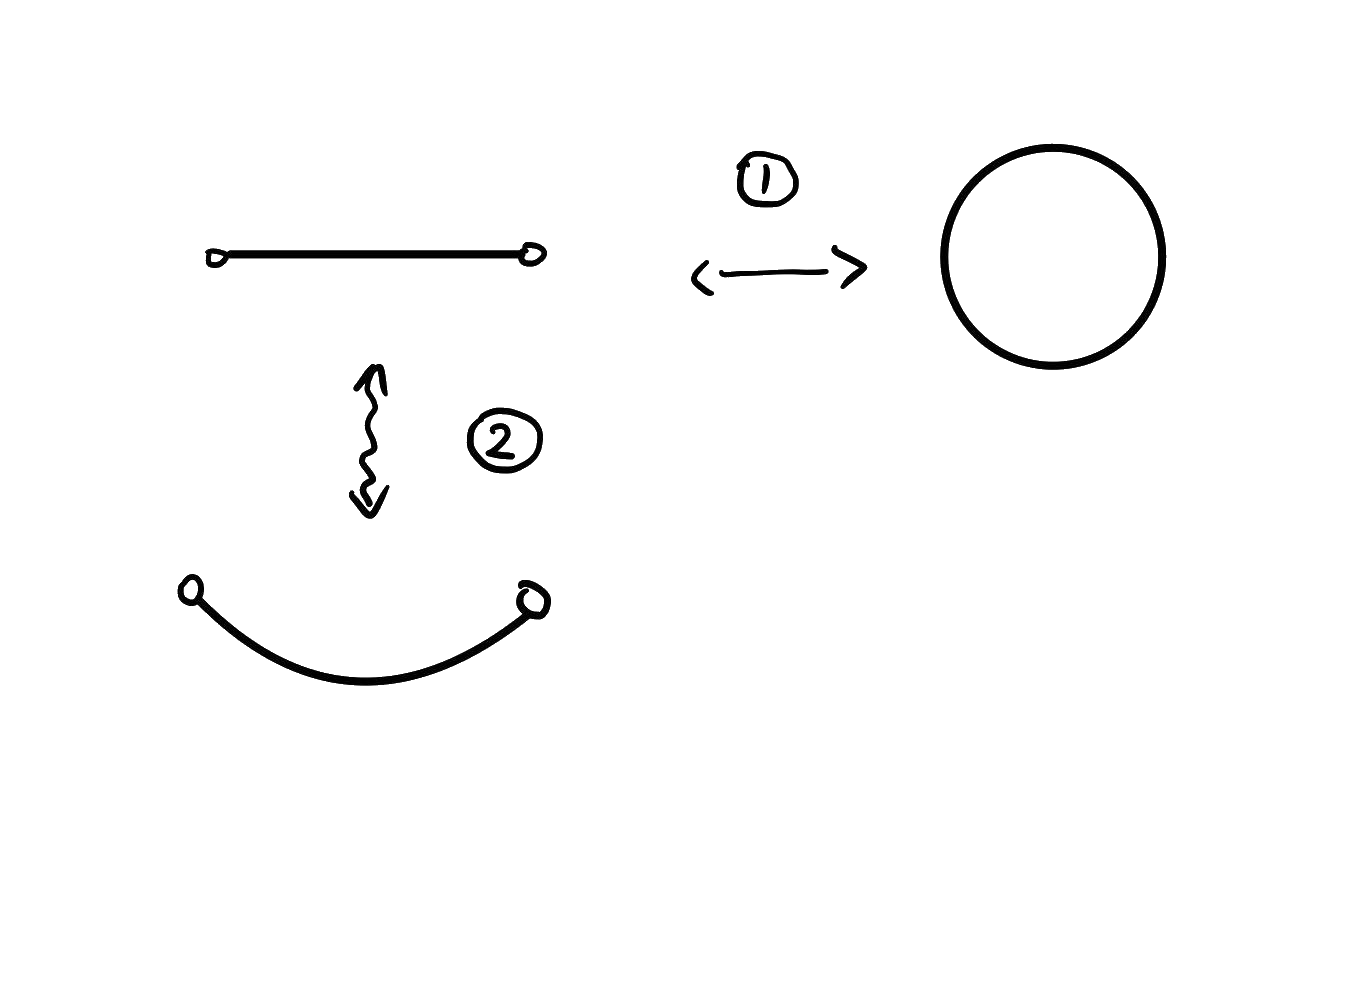
\includegraphics[scale=0.3]{picture/preface/preface_example1.png}
\end{center}

\begin{example}
    (3) differs by ``topology'', but in (4) $\mathbb{S}^2(1)$ is more curve than $\mathbb{S}^2(2)$, even topologically they are the same.(either homeomorphically or diffeomorhically).
\end{example}

\begin{center}
    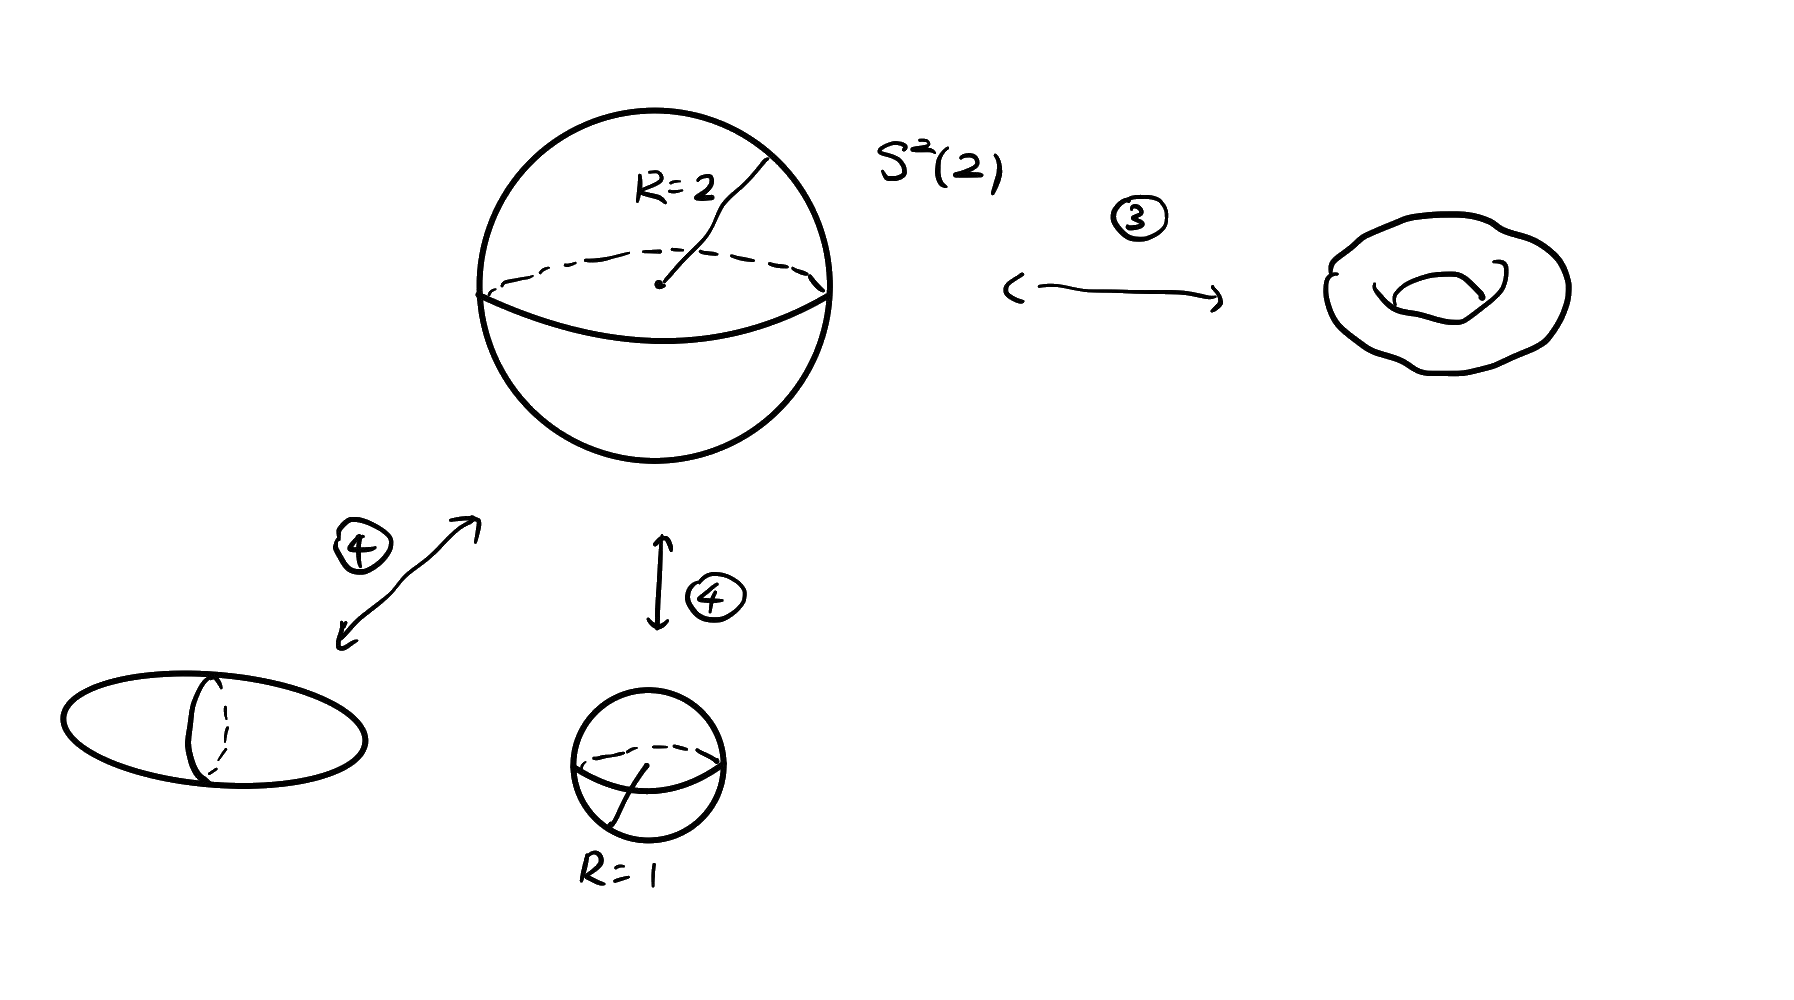
\includegraphics[scale=0.2]{picture/preface/preface_example2.png}
\end{center}

The ``Curved property'' also affects geometric quantities, like length, area, volume, angle between the curves, etc.

\textbf{Local Geometry}: How does a ``curved '' space look like in a neighborhood of a point?
 
\textbf{Global Geometry}: If we know how a ``curved space'' is look like at each point, can we observe how such space looks like globally? This is usually related to topological problems.

$\bullet$ \textbf{Differential}: In this course, by ``smoothness'' we mean the geometric objects we'll study are ``nice'' enough so we can apply ``calculus'' tools to study them.

\textbf{Main tool}: Calculus! We'll see how powerful calculus is in this course, especially, like the maximal principle, integration by parts(stoke's theorem), Taylor's expansion, implicit function theory, etc.

\begin{center}
    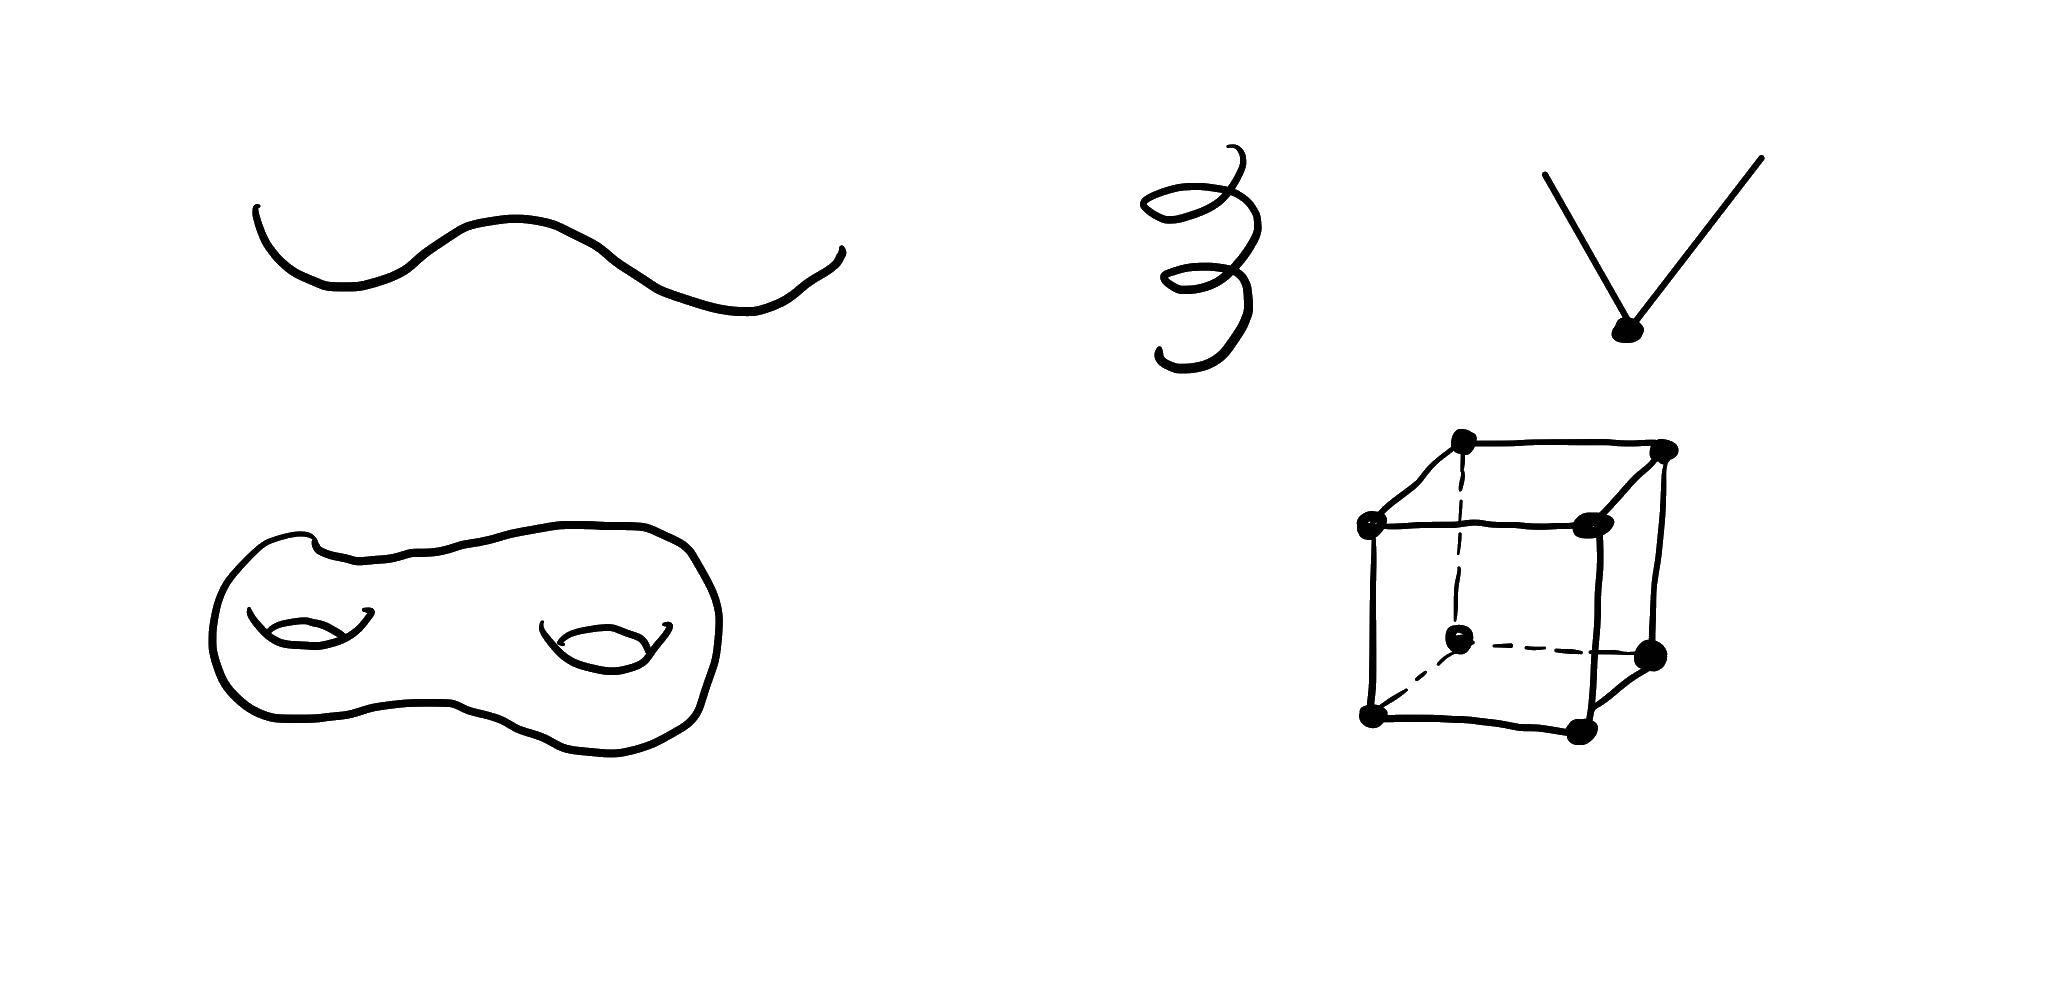
\includegraphics[scale=0.2]{picture/preface/preface_example3.png}
\end{center}

Queastion: How to tell the ``smoothness''?(Need to find good parametrization)Finding a good ``gauge''(that is ``coordinate'') to work with is also an important question in geometry.

$\bullet$Curves: 1-d geometric object.

Surfaces: 2-d geometric object.
\begin{remark}
    In this course, we only focus on curves and surfaces in $\mathbb{R}^3$.However, as a training on preparing for later geometry course, I suggest you also try to think about the ambiant space is $\mathbb{S}^3$ or $\mathbb{H}^3$.

\end{remark}
$\bullet$\textbf{Intrinsic geometry}: Study the geometric object without considering the ambient space. This begins from the Gauss's elegant theorem and was developed by Riemann.
\begin{example}
    Consider the unit sphere $\mathbb{S}^2$

    Extrinsic geometry: view it as $x^2+y^2+z^2=1$ in $\mathbb{R}^3$.

    Intrinsic geometry: $(\theta,\varphi)$ or $(\varphi,\theta)$ are ``essential'' coordinates on $\mathbb{S}^2$. \[
        \dd s^2=\dd \varphi^2+(\sin\varphi)^2 \dd\theta^2
    \]

    (Caution: $(\theta,\varphi)$ is outer normal, while $(\varphi,\theta)$ is inner normal.)
\end{example}
$\bullet$ Useful / Common techniques:
\begin{enumerate}[1)]
    \item Comparison: compare the studied geometric object with ``model space''. It's very important to study examples in geometry. As a suggestion you are expected to spend time to play with $\mathbb{S}^2$.For example: How is $\mathbb{S}^2$ curved? What's the shortest line in $\mathbb{S}^2$? How many symmetries are there on $\mathbb{S}^2$? Can you add ``extra structure'' on$\mathbb{S}^2$ to make it a complex object? Is this ``extra structure'' ``rigid''?What/s the ``moment map'' on $\mathbb{S}^2$? Does there exist a ``holomorphic'' map from $\mathbb{S}^2$ to a torus, or a surface of arbitrary genus? 
 
    If we consider an ``Energy minimizing map'' from $\mathbb{S}^2$ to $\mathbb{S}^2$, what can we say about such map?(It is  holomorphic/antiholomorphic.)
 
    After you have learned Riemann Geometry, you'll see an energy minimizing map from $\mathbb{S}^2$ to a Riemannian manifold must be an angle-preserving map(conformal map).
 
    What kinds of 2-d geometric space could be $\mathbb{S}^2$ ?(this is a global geometry problem.)(\ie\ what kinds of geometric conditions can characterize $\mathbb{S}^2$ ?)
    \item To study higher dimensional objects,it's also important to understand lower dimensional objects, and it's also important to understand lower dimensional objects contained in the studied objects.
    \item Study ``functions'' (more generally sections, including functions, vector fields, differential forms, etc.) on a given geometric object.
\end{enumerate}
\begin{example}
    On a closed surface ( $\mathbb{S}^2$,$\mathbb{T}^2$,$\Sigma_g$)(compact without boundary) there is no non-constant harmonic function.(i.e. $\Delta u=0$)(Analysis will get involved.)
\end{example}
We usually care about those functions related to geometry, such as distance functions, curvature-related functions, etc.
\begin{example}[More trivial than the last one]
    Consider $f''(x)=0$, what can you say of the solution of it when $x$ lies on a line and when $x$ lies on a circle?
\end{example}


\chapter{Differential Geometry of Curves}
\section{Linear algebra convention and its geometric explanation}
\begin{itemize}
    \item We use ``ROW VECTOR'' in this course, \ie\
    \[v\in \mathbb{R}^n, v=(v_1,v_2,\cdots,v_n)\]
    \item let $e_1=(1,0,\cdots,0),\cdots,e_n=(0,\cdots,1)$ be the standard basis, then 
    \[v=\sum_{i=1}^nv^i e_i=
    \begin{bmatrix}
        v^1& v^2& \cdots & v^n
    \end{bmatrix}
    \begin{bmatrix}
        e_1\\
        e_2\\
        \vdots\\
        e_n
    \end{bmatrix}
    \]
    \item $\varphi\colon \mathbb{R}^n\to \mathbb{R}^n$ (non-degenerate) linear map
    \[v\mapsto \varphi(v)=v\cdot A.\]
    This corresponds to the right action of $GL(n,\mathbb{R})$ on $\mathbb{R}^n$.
    \[\Rightarrow \varphi(e_i)=e_j \cdot A=\sum_{i=1}^n A\indices{_j^i}e_i\text{ (taking the j-th row of }A\text{)}\]
    
    \[A\indices{_j^i}\begin{cases}
        \text{upper index: column index}\\
        \text{lower index: row index}
    \end{cases}\]
    \[\Rightarrow \varphi\begin{bmatrix}
        e_1\\
        e_2\\
        \vdots\\
        e_n
    \end{bmatrix}=\begin{bmatrix}
       \varphi( e_1)\\
        \varphi (e_2)\\
        \vdots\\
        \varphi(e_n)
    \end{bmatrix}=\begin{bmatrix}
        e_1\cdot A\\
        e_2\cdot A\\
        \vdots\\
        e_n\cdot A
    \end{bmatrix}=
    A \begin{bmatrix}
        e_1\\
        e_2\\
        \vdots\\
        e_n
    \end{bmatrix}\]
\end{itemize}
\begin{remark}[Important!]
    In row vector convention, a non-degenerate linear map corresponds to the right action of $GL(n,\mathbb{R})$ on $\mathbb{R}^n$. But this induces left action of $GL(n,\mathbb{R})$ on the orthonormal basis (frame) $\{e_1,e_2,\ldots,e_n\}$. This phenomenon provides an important example in differential geometry, which will be explained later in the theory of principle bundle.(\ie\ let $G$ be a lie group, $G\curvearrowright M$ being a right action, where $M$ is a differentiable manifold, then this right action induces a left action of $G$ on the frame bundle of $M$.)
 \end{remark}
 
 
 Let $\{\tilde{e}_1,\ldots,\tilde{e}_n\}$ be another basis of $\mathbb{R}^n$. Let $f$ be the corresponding linear map, \ie\
 \[f\begin{bmatrix}
    e_1\\
    e_2\\
    \vdots\\
    e_n
\end{bmatrix}=\begin{bmatrix}
    \tilde{e}_1\\
    \tilde{e}_2\\
    \vdots\\
    \tilde{e}_n
\end{bmatrix}=B \cdot \begin{bmatrix}
    e_1\\
    e_2\\
    \vdots\\
    e_n
\end{bmatrix}\]
\[\Rightarrow \tilde{e}_k=\sum_{j=1}^n B\indices{_k^j}e_j\]
We compare the matrix of $\varphi$ in terms of $\left\{\tilde{e}_1 \cdots \tilde{e}_n\right\}$
\[
    \varphi\left[\begin{array}{c}\tilde{e}_1 \\ \vdots \\ \tilde{e}_n\end{array}\right]=\varphi\left[B\left[\begin{array}{c}\tilde{e}_1 \\ \vdots \\ e_n\end{array}\right]\right]=B \cdot \varphi\left[\begin{array}{c}e_1 \\ \vdots \\ e_n\end{array}\right]\text{(linearity of }\varphi\text{)}
\]
\[
    =B A\left[\begin{array}{c}
    e_1 \\
    \vdots \\
    e_n
    \end{array}\right]=B A B^{-1}\left[\begin{array}{c}
    \tilde{e}_1 \\
    \vdots \\
    e_n
    \end{array}\right]
\]
Note in this case.
\[
(\varphi \circ f)\left[\begin{array}{c}
e_1 \\
\vdots \\
e_n
\end{array}\right]=B A\left[\begin{array}{c}
e_1 \\
\vdots \\
e_n
\end{array}\right]
\]
In terms of entries,
\begin{align*}
    \varphi(\tilde{e}_k) &=\varphi(\sum_{j=1}^n B\indices{_k^j} e_j)=\sum_{j=1}^n B\indices{_k^j} \varphi(e_j) \quad \text { (linearity) } \\
    &=\sum_{i, j=1}^n B\indices{_k^j} A\indices{_j^i} e_i=\sum_{i,j,p=1}^n B\indices{_k^j} A\indices{_j^i}(B^{-1})\indices{_i^p} \widetilde{e}_p
\end{align*}
\begin{remark}
    This computation tells that the row vector convention yields to the fact that $GL(n,\mathbb{R})$ acting on itself from the right when we consider the action of $GL(n, \mathbb{R})$ on $\mathbb{R}^n$.
    In modern Geometry, it's more common to use column vector as convention. This row vector convention was adopted by S.S. Chern and also Do Cormo's book.
\end{remark}
\section{Parametrized Curves}
\begin{definition}
    Let $I=(a,b)$, if $\alpha\colon I\to \mathbb{R}^3$ is a $C^\infty$ map,
    \[t \mapsto (x(t),y(t),z(t))\]
    then $\alpha(t)$ is a parametrized differentiable curve in $\mathbb{R}^3$. The image of $\alpha$ is called the trace of the curve. 
\end{definition}
\begin{remark}
    \hfill
    \begin{enumerate}[1)]
        \item $a,b$ could be finite number or infinity.
        \item Same curve may have different parametrizations.
        \item The parametrization automatically gives the direction of the motion on the curve.
        \item ``Differentiable'' just means $\alpha(t)$ is a $C^\infty$ \textbf{map}, it does not say the (trace of) curve can not have singularities.
    \end{enumerate}
\end{remark}
\begin{example}
    \hfill
    \begin{enumerate}[(1)]
        \item $\alpha(t)=(t,|t|)$ is not a differentiable curve.
        \begin{center}
            \begin{tikzpicture}
                \draw[domain=-2:0,smooth,variable=\t,black]
                plot (\t,{-\t});
                \draw[domain=0:2,smooth,variable=\t,black]
                plot (\t,\t);    
                \draw (0,0) node{$\bullet$};
                \draw[->] (-2,0) -- (2,0) node[right] {$x$};
                \draw[->] (0,-0.5) -- (0,2.5) node[above] {$y$};
            \end{tikzpicture}
        \end{center}
        \item $\alpha=(t^3,t^2)$ is a differentiable curve. It can be also given by a equation $y^3=x^2$, which is a cuspidal cubic curve.
        \begin{center}
            \begin{tikzpicture}
                \draw[domain=-1.5:1.5,smooth,variable=\t,black]
                plot ({\t^3},{\t*\t});
                \draw (0,0) node{$\bullet$};
                \draw[->] (-2,0) -- (2,0) node[right] {$x$};
                \draw[->] (0,-0.5) -- (0,2.5) node[above] {$y$};
            \end{tikzpicture}
        \end{center}
        \item $\alpha(t)=(t^2-1,t^3-t)$. This parametrization appers in the ``blow-up'' process of $y^2=x^3+x^2$. Here ``blow-up'' is introducing tangents to seperate points.
        \begin{center}
            \begin{tikzpicture}
                \draw[domain=-1.5:1.5,smooth,variable=\t,black]
                plot ({\t*\t-1},{\t^3-\t});
                \draw (0,0) node{$\bullet$};
                \draw[->] (-2,0) -- (2,0) node[right] {$x$};
                \draw[->] (0,-2.5) -- (0,2.5) node[above] {$y$};
            \end{tikzpicture}
        \end{center}
    \end{enumerate}
\end{example}
\begin{remark}
    (2) and (3) above may be the first examples you'll see in an algebraic geometry course.
\end{remark}
\noindent
\textbf{Question}: At the origin, what can you obsefve on (2) and (3)?

\noindent
\textbf{Answer}:
    (2) $\alpha'(0)=0$.
    (3) $\alpha$ is not one to one, but $\alpha'(0)\neq 0$.

\noindent 
\textbf{Question}: Define a differentiable curve in $\mathbb{R}^3$ and $\mathbb{S}^n$.
\begin{remark}
    Among above differentiable parametrizations, (2) and (3) are differentiable curves. However, if we take $\beta(t)=(t,t^{\frac{2}{3}})$, this also parametrizes (2), but it's not a differentiable curve!
\end{remark}
\begin{definition}
    Let $\alpha(t)\colon I\to \mathbb{R}^3$ be a parametrized differentiable curve, then at $t_0\in I$.
    \[ \alpha'(t_0)=(x'(t_0),y'(t_0),z'(t_0))\]
    is the velocity of $\alpha(t)$ at $t_0$.
    \begin{enumerate}[(1)]
        \item If $\alpha'(t_0)\neq 0$, we call $\alpha(t_0)$ a regular point.
        \item If $\alpha'(t_0) = 0$, we call $\alpha(t_0)$ a singular point.
        \item If for all $t\in I$, $\alpha'(t)\neq 0$, we call $\alpha(t)$ a regular curve.
    \end{enumerate}
\end{definition}
\noindent
\textbf{Question}: What can you say about $C^\infty$ parametrization for a regular curve?
\begin{quotation}
Regular curve $\Longleftrightarrow $ at each point, there is a unique tangent line.
\end{quotation}
\begin{example}
$\alpha(t)=(t^3,t^2)$ is not a regular curve. (Since $\alpha'(0)=0$)
\begin{center}
    \begin{tikzpicture}
        \draw[domain=-1.5:1.5,smooth,variable=\t,black]
        plot ({\t^3},{\t*\t});
        \draw (0,0) node{$\bullet$};
        \draw[->] (-2,0) -- (2,0) node[right] {$x$};
        \draw[->] (0,-0.5) -- (0,2.5) node[above] {$y$};
    \end{tikzpicture}
\end{center}
\end{example}
\begin{example}
$\alpha(t)=(t^2-1,t^3,t)$ is a regular curve.
\begin{center}
    \begin{tikzpicture}
        \draw[domain=-1.5:1.5,smooth,variable=\t,black]
        plot ({\t*\t-1},{\t^3-\t});
        \draw (0,0) node{$\bullet$};
        \draw[->] (-2,0) -- (2,0) node[right] {$x$};
        \draw[->] (0,-2.5) -- (0,2.5) node[above] {$y$};
    \end{tikzpicture}
\end{center}
\end{example}
\begin{definition}
Let $\alpha(t)$ be a regular curve, then the tangent line at $t_0$ is \[l(t)=\alpha(t_0)+\alpha'(t_0)(t-t_0))\]
\begin{center}
    \begin{tikzpicture}[scale=1.25]
    \draw (0, -1) .. controls (1.5, 2) and (2, -3) .. (4,1.5)    % 绘制曲线
        node[
            pos = 0.6,    % 设置切点在曲线上的位置
            sloped,    % 设置node按曲线斜率旋转
            anchor = south west
            ] (N) {};
         

    \draw[blue]($(N.south west)!0.6cm!180:(N.south east)$) -- ($(N.south west)!0.6cm!(N.south east)$);
    \draw (0, -1) .. controls (1.5, 2) and (2, -3) .. (4,1.5)
        node[
        pos = 0.2,    % 设置切点在曲线上的位置
        sloped,    % 设置node按曲线斜率旋转
        anchor = south west
        ] (M) {}; 
    \draw[cyan]($(M.south west)!0.6cm!180:(M.south east)$) -- ($(M.south west)!0.6cm!(M.south east)$);
    \draw (0, -1) .. controls (1.5, 2) and (2, -3) .. (4,1.5)
        node[
        pos = 0.9,    % 设置切点在曲线上的位置
        sloped,    % 设置node按曲线斜率旋转
        anchor = south west
        ] (M) {}; 
    \draw($(M.south west)!1cm!180:(M.south east)$) -- ($(M.south west)!1cm!(M.south east)$);
    \end{tikzpicture}
\end{center}
\end{definition}
\begin{definition}
    Let $\alpha(t)$ be a regular curve, the arc-length of $\alpha(t)$ is 
    \[s(t)=\int_{t_0}^t \left|\alpha'(t)\right|\dd t.\]
    Then $s'(t)=\left|\alpha'(t)\right|$
\end{definition}
\textbf{Question} What's $\left|\alpha'(t)\right|$?

 
$\alpha(t)\colon I\to \mathbb{R}^3$ is a curve in $\mathbb{R}^3$. Here on $\mathbb{R}^3$, as the Euclidean space, we always assume the standard Euclidean inner product on it, \ie\ $\forall u=(u_1,u_2,u_3),v=(v_1,v_2,v_3)$
\[\langle u,v\rangle=u_1 v_1+u_2 v_2+ u_3 v_3=\sum_{i,j=1}^3\delta_{ij}u_i v_j\]
Let $\alpha(t)=(x(t),y(t),z(t)),\alpha'(t)=(x'(t),y'(t),z'(t))$, then $\left|\alpha'(t)\right|=\sqrt{\langle\alpha'(t),\alpha'(t)\rangle}$
\begin{exercise}
    Review vector Calculations, such as dot product, cross product and their properties, especially geometric meanie of these calculation, such as length, area, volume, angle, orientation, etc.
\end{exercise}
\noindent
\textbf{Question}: Can you define the arclength of a regular curve in $\mathbb{R}^n$? How about on $\mathbb{S}^n$? \\
$\bullet$ Arclength parameter(an intrinsic parametrization of a curve)
\begin{example}
On a straight line, x=t describes the distance of the point away from the origin.
\begin{center}
    \begin{tikzpicture}
        \draw[->] (-2,0) -- (2,0) node[right] {};
        \draw (-1,0.05) node{$\bullet$};
        \draw (0.2,0.2) node{$t$};
        \draw[->,blue] (-1,0.1)--(0,0.1) node[right] {};
    \end{tikzpicture}
\end{center}
\end{example}
On a general curve, we also want ``some'' parameter, which describes the arclength of point away from the initial point. This can happen iff $|\alpha'(t)|=1$,\ie\ a point on the curve moves in a unit speed.
\[\Rightarrow s(t)=\int_0^t \dd t=t.\]
\textbf{Question}: For a given regular curve $\alpha(t)\colon I\to \mathbb{R}^3$, how to find such parameter?

\noindent 
\textbf{Answer}: $s(t)=\int_{t_0}^t \left|\alpha'(t)\right|\dd t$ is a function in t, and $s'(t)=\left|\alpha'(t)\right|\neq 0$(because the curve is regular). By the implicit function theorem, there is a function 
\[
    t=t(s),t'(s)=\frac{1}{\left|\alpha'(t)\right|}.
\]
This implies that 
\[
    \alpha(t)=\alpha(t(s))=(x(t(s)),y(t(s)),z(t(s)))
\]
\[
    \left|\alpha'(s)\right|=\left|\alpha'(t)t'(s)\right|=\left|\alpha'(t)\right|\left|t'(s)\right|=1
\]

\boxed{\textbf{Convention}} In this course, we only consider differentiable regular curves, which are parametrized by the arclength (for convenience).
\begin{remark}
    In this course, we only consider the curve without self-intersecting points, i.e curves ``embedded into'' $\mathbb{R}^3$. Here ``embedded'' means $d\alpha$ is a linear isomorphism and $\alpha$ is homeomorphic to its image.
\end{remark}

\section{Local theory of a regular space curve}

\begin{goal}
    Describe a space curve by using geometric quantities.
\end{goal}

\begin{ques}
    How to make a space curve? 
\end{ques}
Starting with a straight line, we can bend it and twist it in a given way to
produce a space curve.
\begin{itemize}
    \item Bending the line \(\longrightarrow\) ``curvature''.
    \item Twisting \(\longrightarrow\) ``torsion''.
    \item Their relations are contained in Frenet formula.
    \item Conversely, fundamental theorem of the local theory of curves
        tells, once we're given two function, \(\kappa(s),\tau(s)\), we can
        describe a unique curve in \(\mathbb{R}^3\) up to a rigid motion,
        \st\ \(\kappa(s)\) is its curvature and \(\tau(s)\) is its torsion.
\end{itemize}

\noindent\underline{\bf Recall:} In Calculus, if \(y=f(x)\) represents a curve, then
\(f''(x)\) tells the convexity of the curve. It measures how fast the velocity
changes. It's also related to how straight line is bent.


Let \(\alpha\colon I\to \mathbb{R}^2\) be a regular plane curve, parametrized by
arc length, \ie\ \(|\alpha'(s)|=1\). Then \(\left<\alpha'(s),\alpha''(s)\right> =0\),
and hence \(\alpha''(s)\perp\alpha'(s)\). For a plane curve, we take normal of the
curve to be counterclockwise \(90^\circ\) rotation of the tangent vector.

% Figure fig:w2-plane-curve-eg here

Let \(N\) be the unit normal vector along \(\alpha(s)\), we have \[
    \left<\alpha''(s),N(s)\right> =\pm|\alpha''(s)|
.\] 
\begin{defn}
    The curvature of a plane curve \(\alpha(s)\) is defined as \[
        \kappa(s)=\left<\alpha''(s),N(s)\right>
    .\] 
\end{defn}
\begin{defn}
    Further we denote \(T\) be the unit tangent vector, then the Frenet equation
    of \(\alpha(s)\) is \[
        \begin{cases}
            T'=\kappa N \\
            N'=-\kappa T
        \end{cases}
    .\] Note that \[
        \left<T',N\right> =\kappa\implies \left<T,N'\right> =-\kappa
    .\] 
\end{defn}

\begin{itemize}
    \item \(\kappa>0\implies \) the point on the curve moves counterclockwise
        direction or say ``to its left''.
    \item \(\kappa<0\implies \) the point on the curve moves clockwise direction
        or say ``to its right''.
\end{itemize}

\begin{ques}
    For the curve in \cref{fig:w2-plane-curve-eg}, can you tell where \(\kappa>0\)
    and where \(\kappa<0\) without doing calculation?
\end{ques}

\begin{remark}
    The sign of the curvature of the plane curve is caused by the direction
    convention of the unit normal vector. This could change according to the
    orientation of a curve.
\end{remark}

Next, we take a look at the geometric meaning of \(|\alpha''(s)|\) at some point
\(\alpha(s_0)\). By definition: \[
    |\alpha''(s_0)|=\lim_{h \to 0} \left|\frac{\alpha'(s_0+h)-\alpha'(s_0)}{h}\right|
.\] 
% May be figure here
We have
\begin{align*}
    |\alpha'(s_0+h)-\alpha'(s_0)|
    &= \left(|\alpha'(s_0+h)|^2+|\alpha'(s_0)|^2-2\left<\alpha'(s_0+h),
    \alpha'(s_0)\right> \right)^{\frac{1}{2}} \\
    &= (2-2\cos\theta_h)^{\frac{1}{2}} \\
    &= (2-2(1-\frac{1}{2}\theta_h^2)+\tilde{o}(\theta_h)^4)^{\frac{1}{2}} \\
    &= (\theta_h^2+\tilde{o}(\theta_h)^4)^{\frac{1}{2}}
.\end{align*}
Hence \[
    |\alpha''(s_0)|=\lim_{h \to 0} \left|\frac{\alpha'(s_0+h)-\alpha'(s_0)}{h}\right|
    =\lim_{h \to 0} \left|\frac{\theta_h}{h}\right|=|\theta'(s_0)|
.\] \ie\ \(|\alpha''(s)|\) measures the changing rate of angle of tangents.

\section{Global theory of plane curves}

The global theory is related to ``topology'' of the geometric objects.
For 1-dimensional geometry, \ie\ curves, it's always oriented. And the simplest distinction in topology
is ``open'' and ``closed''.

\begin{definition}[Closed curves]
    \begin{itemize}\hfill
        \item We say
              \(\alpha\colon I=[a,b]\to \mathbb{R}
              ^3\)
              (or \(\mathbb{R}^2\))
              is a closed regular curve, if
              \(\alpha(a)=\alpha(b)\)
              and
              \(\alpha^{(k)}
              (a)=\alpha^{(k)}(b)\)
              (in another word,
              \(\alpha\colon \mathbb{S}^1\to \mathbb{R}^3\)
              is a differentiable curve).
        \item Furthermore, if
              \(\alpha\)
              has no
              self-intersection point other than
              $\alpha(a)=\alpha(b)$,
              then we call $\alpha(s)$ to be a simple closed curve.
    \end{itemize}
\end{definition}
\begin{center}
    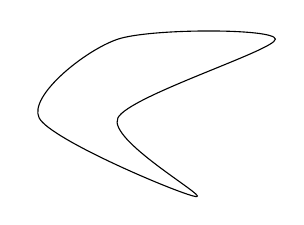
\begin{tikzpicture}
        \draw plot [smooth cycle] coordinates {(0,0) (1,1) (3,1) (1,0) (2,-1)};
    \end{tikzpicture}
\end{center}

\subsection{Isoperimetric inequality}
This is one of the oldest and most famous problem in geometry. It's still attracting mathematicians to investigate such problem in various geometric formulations nowadays.
\begin{question}
    Given a closed plane curve \(C\) with. Let \(D\) be the
    region bounded by \(C\). When does the region have the
    maximal area, if \(C\) is among all the curves with
    fixed length?
\end{question}
\begin{answer}
    \(C\) must be a circle when the maximal area is
    achieved.
\end{answer}
\begin{remark}
    Even though we'll only handle smooth, simple closed
    curves in the following discussion, in general we
    don't have to assume the curve to be simple:
    {\ooalign{$\bigcirc $\cr $\ \ \,\bigcirc $}}
    has less area than $\bigcirc $.(caution: their boundaries are intended to have the same length). Thick about how
        {\ooalign{$\bigcirc $\cr $\ \ \,\bigcirc $}}
    comes from $\bigcirc $.
\end{remark}

\subsubsection*{Proofs of the Isoperimetric inequality}
\begin{proof}1 (Hurwitz's proof) This relies on the ``Wirtinger's inequality''.

    Let $\alpha(t)$ be a closed, simple smooth curve, where $t$ can be any parameter. The length of it is
    \[L=\int_a^b\sqrt{x'(t)^2+y'(t)^2}\dd t.\]

    Observe that we need to find the lower bound of $L^2$.
    Generally, for an integral $L=\int \sqrt{f}\dd t$, H\"older
    inequality (or Cauchy-Schwarz) naturally gives estimate of
    L. Hence, it's natural to find a ``good parameter'' to
    clear. Although the arclength $s$ is a good candidate, it
    turns out in this case that another good parameter is
    \[\theta=\frac{2\pi}{L}s.\]
    $s\in [0,L]\Rightarrow \theta \in [0,2\pi]$.
    (This parameter $\theta$ comes from the ``Wirtinger's inequality', but of course a rescaling of wirtinger's inequality allows us to use $s$ as usual).

    Let's take $\theta=\frac{2\pi}{L}s$, then
    \[\left(\frac{\dd x}{\dd \theta}\right)^2+\left(\frac{\dd y}{\dd \theta}\right)^2=\left(\left(\frac{\dd x}{\dd s}\right)^2+\left(\frac{\dd y}{\dd s}\right)^2\right)\left(\frac{\dd s}{\dd \theta}\right)^2=\left(\frac{L}{2\pi}\right)^2.\]
    \[\Rightarrow \frac{L^2}{2\pi}=\frac{L^2}{4\pi^2}\cdot 2\pi=\int_0^{2\pi}\left(x'(\theta)^2+y'(\theta)^2\right)\dd \theta.\]
    Therefore,
    \begin{align}
        2\left(\frac{L^2}{4\pi}-A\right) & =\int_0^{2\pi}\left(x'(\theta)^2+y'(\theta)^2\right)\dd \theta-2\int_0^{2\pi}x(\theta)y'(\theta)\dd \theta \notag \\
                                         & =\int_0^{2\pi}x'(\theta)^2-x(\theta)^2+\underbrace{(y'(\theta)-x(\theta))^2}_{\ge 0}\dd \theta \notag             \\
                                         & \ge \int_0^{2\pi}x'(\theta)^2-x(\theta)^2 \dd \theta \tag{$\bigstar$}
        .\end{align}
    Now, the proof reduces to the following lemma.

    \begin{lemma}[Wirtinger's inequality]
        Let $f\colon\mathbb{R}\to \mathbb{R}$ be a $2\pi$-periodic smooth
        function and $\int_0^{2\pi}f(\theta)\dd \theta=0$, Then
        \[\int_0^{2\pi}f(\theta)^2\dd \theta\le \int_0^{2\pi}f'(\theta)^2\dd \theta,\]
        and equality holds iff $f(\theta)=a\cos(\theta)+b\sin(\theta)$.
    \end{lemma}
    (Proof of the lemma is left as a homework problem.)

    To apply this to $(\bigstar)$, we need to assume $\int_0^{2\pi}x(\theta)\dd \theta=0$. However, we know the center of mass of the curve is $\left(\frac{\int x(\theta)\dd \theta}{L},\frac{\int y(\theta)\dd \theta}{L}\right)$, and by choosing the origin of $\mathbb{R}^2$ as the center of mass, we can guarantee $\int_0^{2\pi}x(\theta)\dd \theta=0$, this yields $\bigstar\ge 0$, \ie\ $L^2\ge 4\pi A$. Moreover, equality implies
    \[x(\theta)=a\cos(\theta)+b\sin(\theta)\text{ and }y'(\theta)=x(\theta)\Rightarrow\]
    \[y(\theta)=a\sin(\theta)-b\cos(\theta)+c.\]
    So $(x(\theta),y(\theta))$ is a circle.
\end{proof}
\begin{proof}2 (By Schmidt)
    See Do Carmo's book (page 33-35). It will be lectured by TA in a recitation.
\end{proof}
\begin{remark}\hfill
    \begin{enumerate}[(1)]
        \item There are many other proofs of Isoperimetric
              inequality. In the homework 3, we will use a
              modern tool-curve shortening flow to give a proof.
        \item
              \begin{align*}
                  L^2                                                                                & \ge 4 \pi A  \Rightarrow \frac{L^2}{4\pi}\ge A \Rightarrow
                  \frac{L^2}{4\pi^2 r^2}\ge \frac{A}{\pi r^2}(\text{take }r=1)                                                                                    \\
                  \Rightarrow \frac{L}{2\pi}\ge \left(\frac{A}{\pi}\right)^{\frac{1}{2}}\text{\ie\ } &
                  \frac{\text{length of curve}}{\text{length of the unit circle}}
                  \ge \left(\frac{\text{Area bounded by the curve}}{\text{Area of the unit disk}}\right)^{\frac{1}{2}}
                  .\end{align*}
    \end{enumerate}
\end{remark}
$\bullet$ \textbf{Generalization}: Let $E$ be a compact domain in $\mathbb{R}^n$ with smooth boundary $\partial E$, then
\[
    \frac{\text{Area}(\partial E)}{\text{Area of the unit sphere in }\mathbb
        {R}^n}\ge \left(\frac{\text{Volume of }E}{\text{Volume of the unit
            ball}}\right)^{\frac{n-1}{n}}
\]
For simplicity, we write
\[
    \frac{|\partial E|}{\partial B^n} \ge \left(\frac{|E|}{|B^n|}\right)^
    {\frac{n-1}{n}}.
\]
\begin{question}
    Can you propose some generalizations of isoperimetric inequality?
    Isoperimetric inequality is one of the motivation to develop geometric measure theory!
\end{question}
\subsection{Four-vertex theorem}
\begin{theorem}\label{thm:four-vertex theorem}
    A simple closed convex plane curve has at least four vertices.
\end{theorem}
\begin{remark}
    The four-vertex theorem holds also for simple closed non-convex curves.
    The proof is harder, however.
\end{remark}
\begin{definition}[Convex curves]
    $\alpha(s)$ is a convex curve, if at each point $\alpha(s_0)$, the whole curve lies on the same side of the tangent line.
\end{definition}




\tikzset{every picture/.style={line width=0.75pt}} %set default line width to 0.75pt        

\begin{tikzpicture}[x=0.75pt,y=0.75pt,yscale=-0.9,xscale=0.9]
    %uncomment if require: \path (0,300); %set diagram left start at 0, and has height of 300

    %Shape: Ellipse [id:dp6953189046620603] 
    \draw   (48.45,88.74) .. controls (48.45,62.65) and (86.87,41.5) .. (134.27,41.5) .. controls (181.67,41.5) and (220.09,62.65) .. (220.09,88.74) .. controls (220.09,114.83) and (181.67,135.97) .. (134.27,135.97) .. controls (86.87,135.97) and (48.45,114.83) .. (48.45,88.74) -- cycle ;
    %Straight Lines [id:da8702738615642636] 
    \draw    (220.09,57.77) -- (222.1,161) ;
    %Straight Lines [id:da3706263383184776] 
    \draw    (64.66,42.75) -- (221.43,39) ;
    %Straight Lines [id:da3054598329478624] 
    \draw    (39.2,129.09) -- (242.2,145.36) ;
    %Straight Lines [id:da15509227924350344] 
    \draw    (41.21,44.63) -- (57.96,149.74) ;
    %Curve Lines [id:da726485353707341] 
    \draw    (265.2,30) .. controls (274.4,117) and (369.2,233) .. (398.2,30) ;
    %Straight Lines [id:da03667314517418263] 
    \draw    (265.2,47) -- (319.2,187) ;
    %Straight Lines [id:da7191564753420123] 
    \draw    (247.2,131) -- (416.2,153) ;
    %Straight Lines [id:da8951764820712218] 
    \draw    (433.2,59) -- (335.2,162) ;
    %Curve Lines [id:da7789942846266422] 
    \draw    (466.2,160) .. controls (478.4,60) and (608.2,50) .. (610.2,172) ;
    %Straight Lines [id:da306587637969457] 
    \draw    (455,71) -- (630.2,95) ;
    %Straight Lines [id:da1811450298421866] 
    \draw    (532.2,39) -- (442,175) ;
    %Straight Lines [id:da35817044779115514] 
    \draw    (544,60) -- (644,160) ;

\end{tikzpicture}
The convex curve has the following useful characterization.
\begin{proposition}
    $\alpha(s)$ is a convex curve $\Leftrightarrow $ at each point $\alpha(s_0)$, only one of the following holds:
    \begin{quotation}
        For all $s\in I$, either $(\alpha(s)-\alpha(s_0))\cdot \vec{n}(s_0)\ge 0$ or $(\alpha(s)-\alpha(s_0))\cdot \vec{n}(s_0)\le 0$.
    \end{quotation}
    Geometrically, this means at a convex point, the angle between vector $\alpha(s)-\alpha(s_0)$ and $\vec{n}(s_0)$ should be either $[0,\frac{\pi}{2}]$ or $[\pi,\frac{3\pi}{2}]$.
\end{proposition}
\begin{example}\hfill

    \tikzset{every picture/.style={line width=0.75pt}} %set default line width to 0.75pt        

    \begin{center}
        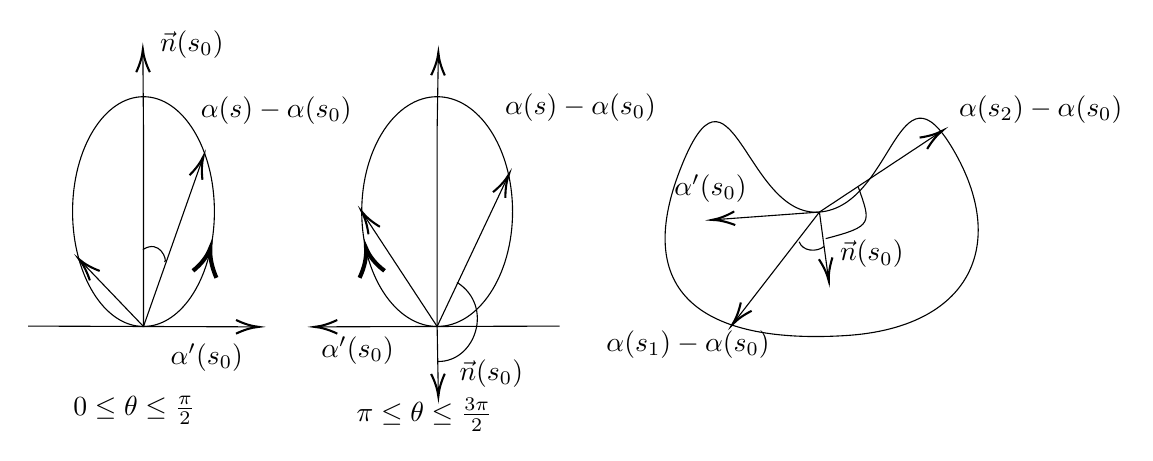
\begin{tikzpicture}[x=0.75pt,y=0.75pt,yscale=-1,xscale=1]
            %uncomment if require: \path (0,300); %set diagram left start at 0, and has height of 300

            %Shape: Ellipse [id:dp7591861540053348] 
            \draw   (52.86,98.9) .. controls (52.86,68.33) and (68.16,43.55) .. (87.03,43.55) .. controls (105.9,43.55) and (121.2,68.33) .. (121.2,98.9) .. controls (121.2,129.48) and (105.9,154.26) .. (87.03,154.26) .. controls (68.16,154.26) and (52.86,129.48) .. (52.86,98.9) -- cycle ;
            %Straight Lines [id:da06336028525669235] 
            \draw    (31.5,154.07) -- (140.55,154.44) ;
            \draw [shift={(142.55,154.45)}, rotate = 180.19] [color={rgb, 255:red, 0; green, 0; blue, 0 }  ][line width=0.75]    (10.93,-3.29) .. controls (6.95,-1.4) and (3.31,-0.3) .. (0,0) .. controls (3.31,0.3) and (6.95,1.4) .. (10.93,3.29)   ;
            %Straight Lines [id:da8240848008506814] 
            \draw    (87.03,154.26) -- (115.29,74.05) ;
            \draw [shift={(115.95,72.17)}, rotate = 109.41] [color={rgb, 255:red, 0; green, 0; blue, 0 }  ][line width=0.75]    (10.93,-3.29) .. controls (6.95,-1.4) and (3.31,-0.3) .. (0,0) .. controls (3.31,0.3) and (6.95,1.4) .. (10.93,3.29)   ;
            %Straight Lines [id:da8702455490360739] 
            \draw    (87.03,154.26) -- (87.03,59.36) -- (86.74,22.8) ;
            \draw [shift={(86.73,20.8)}, rotate = 89.55] [color={rgb, 255:red, 0; green, 0; blue, 0 }  ][line width=0.75]    (10.93,-3.29) .. controls (6.95,-1.4) and (3.31,-0.3) .. (0,0) .. controls (3.31,0.3) and (6.95,1.4) .. (10.93,3.29)   ;
            %Straight Lines [id:da8932284835920707] 
            \draw    (87.03,154.26) -- (57.39,123.32) ;
            \draw [shift={(56,121.88)}, rotate = 46.23] [color={rgb, 255:red, 0; green, 0; blue, 0 }  ][line width=0.75]    (10.93,-3.29) .. controls (6.95,-1.4) and (3.31,-0.3) .. (0,0) .. controls (3.31,0.3) and (6.95,1.4) .. (10.93,3.29)   ;
            \draw  [line width=1.5]  (110.87,127.44) .. controls (114.91,124.19) and (117.7,120.57) .. (119.23,116.56) .. controls (118.95,120.94) and (119.93,125.68) .. (122.16,130.8) ;
            %Shape: Ellipse [id:dp3057067643925675] 
            \draw   (264.85,98.9) .. controls (264.85,68.33) and (248.58,43.55) .. (228.51,43.55) .. controls (208.45,43.55) and (192.18,68.33) .. (192.18,98.9) .. controls (192.18,129.48) and (208.45,154.26) .. (228.51,154.26) .. controls (248.58,154.26) and (264.85,129.48) .. (264.85,98.9) -- cycle ;
            %Straight Lines [id:da7048479708357958] 
            \draw    (287.55,154.07) -- (171.47,154.44) ;
            \draw [shift={(169.47,154.45)}, rotate = 359.82] [color={rgb, 255:red, 0; green, 0; blue, 0 }  ][line width=0.75]    (10.93,-3.29) .. controls (6.95,-1.4) and (3.31,-0.3) .. (0,0) .. controls (3.31,0.3) and (6.95,1.4) .. (10.93,3.29)   ;
            %Straight Lines [id:da9292206875165037] 
            \draw    (228.51,154.26) -- (262.22,82.86) ;
            \draw [shift={(263.07,81.05)}, rotate = 115.27] [color={rgb, 255:red, 0; green, 0; blue, 0 }  ][line width=0.75]    (10.93,-3.29) .. controls (6.95,-1.4) and (3.31,-0.3) .. (0,0) .. controls (3.31,0.3) and (6.95,1.4) .. (10.93,3.29)   ;
            %Straight Lines [id:da8265464948656487] 
            \draw    (228.51,154.26) -- (228.51,59.36) -- (229.07,24.31) ;
            \draw [shift={(229.1,22.31)}, rotate = 90.91] [color={rgb, 255:red, 0; green, 0; blue, 0 }  ][line width=0.75]    (10.93,-3.29) .. controls (6.95,-1.4) and (3.31,-0.3) .. (0,0) .. controls (3.31,0.3) and (6.95,1.4) .. (10.93,3.29)   ;
            %Straight Lines [id:da8724360322486144] 
            \draw    (228.51,154.26) -- (193.28,100.58) ;
            \draw [shift={(192.18,98.9)}, rotate = 56.72] [color={rgb, 255:red, 0; green, 0; blue, 0 }  ][line width=0.75]    (10.93,-3.29) .. controls (6.95,-1.4) and (3.31,-0.3) .. (0,0) .. controls (3.31,0.3) and (6.95,1.4) .. (10.93,3.29)   ;
            \draw  [line width=1.5]  (203.16,127.44) .. controls (198.86,124.19) and (195.9,120.57) .. (194.28,116.56) .. controls (194.56,120.94) and (193.53,125.68) .. (191.15,130.8) ;
            %Straight Lines [id:da3485129106090552] 
            \draw    (228.51,154.26) -- (229.07,186) ;
            \draw [shift={(229.1,188)}, rotate = 269] [color={rgb, 255:red, 0; green, 0; blue, 0 }  ][line width=0.75]    (10.93,-3.29) .. controls (6.95,-1.4) and (3.31,-0.3) .. (0,0) .. controls (3.31,0.3) and (6.95,1.4) .. (10.93,3.29)   ;
            %Shape: Polygon Curved [id:ds10755820169219077] 
            \draw   (345.25,79.55) .. controls (369.98,14.77) and (376.88,101.99) .. (412.7,99.13) .. controls (448.52,96.27) and (450.16,23.06) .. (477.14,69) .. controls (504.12,114.95) and (485.38,154.86) .. (425.44,158.63) .. controls (365.49,162.4) and (320.53,144.32) .. (345.25,79.55) -- cycle ;
            %Straight Lines [id:da35610041851976515] 
            \draw    (412.7,99.13) -- (362.99,102.75) ;
            \draw [shift={(360.99,102.9)}, rotate = 355.83] [color={rgb, 255:red, 0; green, 0; blue, 0 }  ][line width=0.75]    (10.93,-3.29) .. controls (6.95,-1.4) and (3.31,-0.3) .. (0,0) .. controls (3.31,0.3) and (6.95,1.4) .. (10.93,3.29)   ;
            %Straight Lines [id:da6090255533817175] 
            \draw    (412.7,99.13) -- (416.92,130.29) ;
            \draw [shift={(417.19,132.27)}, rotate = 262.27] [color={rgb, 255:red, 0; green, 0; blue, 0 }  ][line width=0.75]    (10.93,-3.29) .. controls (6.95,-1.4) and (3.31,-0.3) .. (0,0) .. controls (3.31,0.3) and (6.95,1.4) .. (10.93,3.29)   ;
            %Straight Lines [id:da9846059751183915] 
            \draw    (412.7,99.13) -- (371.96,151.78) ;
            \draw [shift={(370.73,153.36)}, rotate = 307.73] [color={rgb, 255:red, 0; green, 0; blue, 0 }  ][line width=0.75]    (10.93,-3.29) .. controls (6.95,-1.4) and (3.31,-0.3) .. (0,0) .. controls (3.31,0.3) and (6.95,1.4) .. (10.93,3.29)   ;
            %Straight Lines [id:da9899745827591568] 
            \draw    (412.7,99.13) -- (470.23,61.07) ;
            \draw [shift={(471.9,59.96)}, rotate = 146.51] [color={rgb, 255:red, 0; green, 0; blue, 0 }  ][line width=0.75]    (10.93,-3.29) .. controls (6.95,-1.4) and (3.31,-0.3) .. (0,0) .. controls (3.31,0.3) and (6.95,1.4) .. (10.93,3.29)   ;
            %Curve Lines [id:da7720258932280717] 
            \draw    (86.73,117.21) .. controls (94.97,111.93) and (98.72,122.48) .. (97.22,123.23) ;
            %Curve Lines [id:da3500113291593643] 
            \draw    (228.81,171.13) .. controls (247.09,171.43) and (256.08,144.32) .. (238.1,133.02) ;
            %Curve Lines [id:da041829079173997474] 
            \draw    (402.96,113.44) .. controls (404.45,117.96) and (411.2,118.71) .. (414.94,115.7) ;
            %Curve Lines [id:da01241211464079428] 
            \draw    (415.69,111.93) .. controls (438.92,105.91) and (437.43,104.4) .. (431.43,87.08) ;

            % Text Node
            \draw (98.78,161.33) node [anchor=north west][inner sep=0.75pt]    {$\alpha '( s_{0})$};
            % Text Node
            \draw (113.4,42.15) node [anchor=north west][inner sep=0.75pt]    {$\alpha ( s) -\alpha ( s_{0})$};
            % Text Node
            \draw (51.95,186.49) node [anchor=north west][inner sep=0.75pt]    {$0\leq \theta \leq \frac{\pi }{2}$};
            % Text Node
            \draw (171.47,157.85) node [anchor=north west][inner sep=0.75pt]    {$\alpha '( s_{0})$};
            % Text Node
            \draw (260.02,40.68) node [anchor=north west][inner sep=0.75pt]    {$\alpha ( s) -\alpha ( s_{0})$};
            % Text Node
            \draw (93.72,10.56) node [anchor=north west][inner sep=0.75pt]    {$\vec{n}( s_{0})$};
            % Text Node
            \draw (238.06,169.13) node [anchor=north west][inner sep=0.75pt]    {$\vec{n}( s_{0})$};
            % Text Node
            \draw (188.45,187.51) node [anchor=north west][inner sep=0.75pt]    {$\pi \leq \theta \leq \frac{3\pi }{2}$};
            % Text Node
            \draw (341.49,79.86) node [anchor=north west][inner sep=0.75pt]    {$\alpha '( s_{0})$};
            % Text Node
            \draw (421.4,111.4) node [anchor=north west][inner sep=0.75pt]    {$\vec{n}( s_{0})$};
            % Text Node
            \draw (308.84,155.08) node [anchor=north west][inner sep=0.75pt]    {$\alpha ( s_{1}) -\alpha ( s_{0})$};
            % Text Node
            \draw (478.76,41.59) node [anchor=north west][inner sep=0.75pt]    {$\alpha ( s_{2}) -\alpha ( s_{0})$};

        \end{tikzpicture}
    \end{center}
\end{example}
\begin{example}
    $\alpha(t)=\left((1+2\cos t)\cos t,(1+2\cos t)\sin t\right),~ t\in \mathbb{R}.$

    \begin{center}
        \begin{tikzpicture}
            \draw[black!50, thin, ->] (0, -2) -- (0, 2) ;
            \draw[black!50, thin, ->] (-2, 0) -- (2, 0) ;
            \draw[smooth,domain=-190:190,variable=\t]
            plot ({(1+2*cos(\t))*cos(\t)},{(1+2*cos(\t))*sin(\t)});
        \end{tikzpicture}
    \end{center}
\end{example}
\begin{proposition}
    \label{week3_prop2}
    $\alpha(s)$ is a simple closed curve, then
    \begin{center}
        $\alpha(s)$ is convex $\Leftrightarrow $ $k(s)\ge 0~\forall s$ or $k(s)\le 0~\forall s$.
    \end{center}
\end{proposition}
Previously, we have seen that $k(s)$ measures the rate of change
of the angle between tangent vectors. Let's see another similar application.
Let $\alpha(s)$ be parametrized by arclength, then $t(s)\equiv\alpha'(s)$
is a unit tangent vector, \ie\ $|t(s)|=1$.
\begin{center}



    \tikzset{every picture/.style={line width=0.75pt}} %set default line width to 0.75pt        

    \begin{tikzpicture}[x=0.75pt,y=0.75pt,yscale=-0.9,xscale=0.9]
        %uncomment if require: \path (0,300); %set diagram left start at 0, and has height of 300

        %Shape: Polygon Curved [id:ds0026171910463155257] 
        \draw   (73,110) .. controls (79.2,96.6) and (52.2,71.6) .. (99.2,76.6) .. controls (146.2,81.6) and (120.8,135.4) .. (163,110) .. controls (205.2,84.6) and (201.2,85.6) .. (235.2,86.6) .. controls (269.2,87.6) and (307.93,168.02) .. (278.2,187.6) .. controls (248.47,207.18) and (251.2,173.6) .. (223.2,154.6) .. controls (195.2,135.6) and (170.2,198.6) .. (132.2,204.6) .. controls (94.2,210.6) and (61.2,223.6) .. (39.2,171.6) .. controls (17.2,119.6) and (66.8,123.4) .. (73,110) -- cycle ;
        %Straight Lines [id:da28106330439471616] 
        \draw    (163,110) -- (128.91,130.57) ;
        \draw [shift={(127.2,131.6)}, rotate = 328.9] [color={rgb, 255:red, 0; green, 0; blue, 0 }  ][line width=0.75]    (10.93,-3.29) .. controls (6.95,-1.4) and (3.31,-0.3) .. (0,0) .. controls (3.31,0.3) and (6.95,1.4) .. (10.93,3.29)   ;
        %Straight Lines [id:da5458817060478207] 
        \draw    (44.2,189.6) -- (82.68,222.3) ;
        \draw [shift={(84.2,223.6)}, rotate = 220.36] [color={rgb, 255:red, 0; green, 0; blue, 0 }  ][line width=0.75]    (10.93,-3.29) .. controls (6.95,-1.4) and (3.31,-0.3) .. (0,0) .. controls (3.31,0.3) and (6.95,1.4) .. (10.93,3.29)   ;
        %Straight Lines [id:da6770916754212748] 
        \draw    (287,174) -- (303.63,118.42) ;
        \draw [shift={(304.2,116.5)}, rotate = 106.65] [color={rgb, 255:red, 0; green, 0; blue, 0 }  ][line width=0.75]    (10.93,-3.29) .. controls (6.95,-1.4) and (3.31,-0.3) .. (0,0) .. controls (3.31,0.3) and (6.95,1.4) .. (10.93,3.29)   ;
        %Straight Lines [id:da6027951537470264] 
        \draw    (73,110) -- (60.97,138.66) ;
        \draw [shift={(60.2,140.5)}, rotate = 292.77] [color={rgb, 255:red, 0; green, 0; blue, 0 }  ][line width=0.75]    (10.93,-3.29) .. controls (6.95,-1.4) and (3.31,-0.3) .. (0,0) .. controls (3.31,0.3) and (6.95,1.4) .. (10.93,3.29)   ;
        %Shape: Circle [id:dp7864834656043427] 
        \draw   (416,151.6) .. controls (416,110.12) and (449.62,76.5) .. (491.1,76.5) .. controls (532.58,76.5) and (566.2,110.12) .. (566.2,151.6) .. controls (566.2,193.08) and (532.58,226.7) .. (491.1,226.7) .. controls (449.62,226.7) and (416,193.08) .. (416,151.6) -- cycle ;
        %Straight Lines [id:da03492115814864438] 
        \draw    (491.1,151.6) -- (653.2,152.49) ;
        \draw [shift={(655.2,152.5)}, rotate = 180.31] [color={rgb, 255:red, 0; green, 0; blue, 0 }  ][line width=0.75]    (10.93,-3.29) .. controls (6.95,-1.4) and (3.31,-0.3) .. (0,0) .. controls (3.31,0.3) and (6.95,1.4) .. (10.93,3.29)   ;
        %Straight Lines [id:da32329772473464935] 
        \draw    (491.1,151.6) -- (489.23,22.5) ;
        \draw [shift={(489.2,20.5)}, rotate = 89.17] [color={rgb, 255:red, 0; green, 0; blue, 0 }  ][line width=0.75]    (10.93,-3.29) .. controls (6.95,-1.4) and (3.31,-0.3) .. (0,0) .. controls (3.31,0.3) and (6.95,1.4) .. (10.93,3.29)   ;
        %Straight Lines [id:da277337811629643] 
        \draw    (491.1,151.6) -- (537.92,95.04) ;
        \draw [shift={(539.2,93.5)}, rotate = 129.62] [color={rgb, 255:red, 0; green, 0; blue, 0 }  ][line width=0.75]    (10.93,-3.29) .. controls (6.95,-1.4) and (3.31,-0.3) .. (0,0) .. controls (3.31,0.3) and (6.95,1.4) .. (10.93,3.29)   ;
        %Straight Lines [id:da5646379423765395] 
        \draw    (491.1,151.6) -- (428.89,112.56) ;
        \draw [shift={(427.2,111.5)}, rotate = 32.11] [color={rgb, 255:red, 0; green, 0; blue, 0 }  ][line width=0.75]    (10.93,-3.29) .. controls (6.95,-1.4) and (3.31,-0.3) .. (0,0) .. controls (3.31,0.3) and (6.95,1.4) .. (10.93,3.29)   ;
        %Straight Lines [id:da018784269523367092] 
        \draw    (491.1,151.6) -- (428.88,191.42) ;
        \draw [shift={(427.2,192.5)}, rotate = 327.38] [color={rgb, 255:red, 0; green, 0; blue, 0 }  ][line width=0.75]    (10.93,-3.29) .. controls (6.95,-1.4) and (3.31,-0.
        3) .. (0,0) .. controls (3.31,0.3) and (6.95,1.4) .. (10.93,3.29)   ;
        %Straight Lines [id:da14325774903874766] 
        \draw    (491.1,151.6) -- (517.48,219.64) ;
        \draw [shift={(518.2,221.5)}, rotate = 248.81] [color={rgb, 255:red, 0; green, 0; blue, 0 }  ][line width=0.75]    (10.93,-3.29) .. controls (6.95,-1.4) and (3.31,-0.3) .. (0,0) .. controls (3.31,0.3) and (6.95,1.4) .. (10.93,3.29)   ;
        %Curve Lines [id:da620705552589145] 
        \draw    (528.2,151.5) .. controls (528.2,137.5) and (527.2,137.5) .. (515.15,122.55) ;

        % Text Node
        \draw (296,175.4) node [anchor=north west][inner sep=0.75pt]    {$(1)$};
        % Text Node
        \draw (138,89.4) node [anchor=north west][inner sep=0.75pt]    {$( 2)$};
        % Text Node
        \draw (42,93.4) node [anchor=north west][inner sep=0.75pt]    {$( 3)$};
        % Text Node
        \draw (635,161.4) node [anchor=north west][inner sep=0.75pt]    {$x$};
        % Text Node
        \draw (496,13.4) node [anchor=north west][inner sep=0.75pt]    {$y$};
        % Text Node
        \draw (506,134.4) node [anchor=north west][inner sep=0.75pt]    {$\theta $};
        % Text Node
        \draw (537,68.4) node [anchor=north west][inner sep=0.75pt]    {$( 1)$};
        % Text Node
        \draw (396,98.4) node [anchor=north west][inner sep=0.75pt]    {$( 2)$};
        % Text Node
        \draw (394,195.4) node [anchor=north west][inner sep=0.75pt]    {$( 3)$};
        % Text Node
        \draw (524,229.4) node [anchor=north west][inner sep=0.75pt]    {$( 4)$};


    \end{tikzpicture}
\end{center}
Let $\theta$ be the angle between $t(s)$ and the $x$-axis, \ie\ $t(s)=(\cos \theta,\sin \theta)$
\[
    \left. \begin{array}{lll}
        t'(s)=(-\sin \theta,\cos \theta)\dfrac{\dd \theta}{\dd s}=
        \dfrac{\dd \theta}{\dd s}\cdot\vec{n} \\
        \text{on the other hand, }t'(s)=k\cdot\vec{n}
    \end{array}\right\}
    \Rightarrow \boxed{k(s)=\frac{\dd \theta}{\dd s}}
    .\]
As an application, if $k(s)\not\equiv 0$, then $s=s(\theta)$
is defined so that $\frac{\dd s}{\dd \theta}=\frac{1}{k}$,
\ie\ $\theta$ can be used as a parameter
of $\alpha(s)$. Such $\theta$ is called the angle parameter.\\
{\LARGE\textbf{!}} In the study of geometry, the sign of the curvature is a
very important thing to keep in mind.
\begin{definition}
    Let $\alpha\colon I\to \mathbb{R}^3$ be a regular curve. The point at
    which $k'(t_0)=0$ is called a vertex of $\alpha$.(critical point of
    the curvature $k(t)$)
\end{definition}
\begin{proof}[Proof of \cref{week3_prop2}]\hfill

    \textbf{Claim 1}: $\alpha(s)$ is Globally convex $\Rightarrow$ either $k\ge 0$ or $k\le 0$ locally for all $s$.

    W.L.O.G., we assume $c$ is oriented counterclockwise, $\vec{n}$ is the
    inner unit normal vector. We'll show
    \begin{center}
        convex$\Rightarrow k\ge 0$ for all s.
    \end{center}

    Assuming not, then $\exists s_0$ such that $k(s_0)<0$. By the
    continuity of k(s), we can assume $k(s_0)=\min k(s)$. Establish a
    coordinate system at $\alpha(s_0)$ such that $\alpha(s_0)$ is the
    origin, $\alpha'(s_0)$ corresponds to the $x$-axis and $\vec{n}(s_0)$
    to the $y$-axis. We'll show that $\exists s_1,s_2$ such that
    \[\langle \alpha(s_1),\vec{n}(s_0)\rangle<0,\quad
        \langle \alpha(s_2),\vec{n}(s_0)\rangle>0.\]
    Consider the function
    \[f(s)=\langle \alpha''(s),\vec{n}(s_0)\rangle,\]
    then $f(s_0)=k(s_0)\le 0$, which implies that there exists a neighborhood
    $I_\epsilon=(s_0-\epsilon,s_0+\epsilon)$, so that $f(s)<0$ for $s\in I_\epsilon$.
    \[\Rightarrow \langle \alpha''(s),\vec{n}(s_0)\rangle<0
        \Rightarrow \langle \alpha'(s),\vec{n}(s_0)\rangle<
        \langle \alpha(s_0),\vec{n}(s_0)\rangle=0
    \]
    \[\Rightarrow \langle \alpha(s),\vec{n}(s_0)\rangle<
        \langle \alpha(s_0),\vec{n}(s_0)\rangle=0
        .\]
    So there exists an $s_1$ such that $\langle \alpha(s_1),\vec{n}(s_0)\rangle<0.$

    If for all $s\in I$, $\langle \alpha(s),\vec{n}(s_0)\rangle\le 0$, then this means that all points lie on the opposite side of $\vec{n}$. Hence, $\vec{n}$ is ``outer'' normal, a contradiction to our assumption on the direction of $\vec{n}$. So $\exists s_2$ such that $\alpha(s_2)>0$. But this contradicts the assumption on convexity.

    \textbf{Claim 2}: $k\ge 0 \Rightarrow$ global convexity.

    If not, there exists an $s_0$ such that the curve has points on both sides of the tangent line of $\alpha(s_0)$. Consider the height function
    \[h(s)=\langle \alpha(s)-\alpha(s_0),\vec{n}(s_0)\rangle,\]
    then $\exists~s_1, s_2$ such that $h(s_1)<0=h(s_0)<h(s_2)$.
    We can assume that $s_0<s_1<s_2<s_0+l$, where $l$ is the length of $\alpha(s)$. By the continuity of $h$, we can further assume
    \begin{align*}
                    & h(s_1)=\min h(s),~ h(s_2)=\max h(s).            \\
        \Rightarrow & h'(s_1)=\langle\alpha'(s_1),\vec{n}(s_0)\rangle
        =0 \Rightarrow \alpha'(s_1) \perp \vec{n}(s_0)                \\
                    & h'(s_2)=\langle\alpha'(s_2),\vec{n}(s_0)\rangle
        =0 \Rightarrow  \alpha'(s_2) \perp \vec{n}(s_0)
        ,\end{align*}
    and we also know $\alpha'(s_0)\perp \vec{n}(s_0)$.

    $\therefore$ at least two of $\alpha^{\prime} ( s_0), \alpha^{\prime}(s_1), \alpha^{\prime} (s_2)$ have the same direction. Let's assume.
    \[\alpha^{\prime}\left(s_0\right)=\alpha^{\prime}\left(s_1\right) \quad(\because \text{they have the same length})\]
    Note that they are unit vectors, \ie\ images are on $\mathbb{S}^{1}$.
    \begin{center}
        \tikzset{every picture/.style={line width=0.75pt}} %set default line width to 0.75pt        

        \begin{tikzpicture}[x=0.75pt,y=0.75pt,yscale=-1,xscale=1]
            %uncomment if require: \path (0,300); %set diagram left start at 0, and has height of 300

            %Shape: Axis 2D [id:dp1022754048671688] 
            \draw [color={rgb, 255:red, 155; green, 155; blue, 155 }  ,draw opacity=1 ] (260,143.65) -- (439.2,143.65)(349.2,49.5) -- (349.2,245.5) (432.2,138.65) -- (439.2,143.65) -- (432.2,148.65) (344.2,56.5) -- (349.2,49.5) -- (354.2,56.5)  ;
            %Shape: Circle [id:dp3709466656659819] 
            \draw   (293.83,143.65) .. controls (293.83,113.07) and (318.62,88.28) .. (349.2,88.28) .. controls (379.78,88.28) and (404.58,113.07) .. (404.58,143.65) .. controls (404.58,174.23) and (379.78,199.03) .. (349.2,199.03) .. controls (318.62,199.03) and (293.83,174.23) .. (293.83,143.65) -- cycle ;
            %Straight Lines [id:da5170953335810249] 
            \draw    (349.2,143.65) -- (387.72,108.84) ;
            \draw [shift={(389.2,107.5)}, rotate = 137.89] [color={rgb, 255:red, 0; green, 0; blue, 0 }  ][line width=0.75]    (10.93,-3.29) .. controls (6.95,-1.4) and (3.31,-0.3) .. (0,0) .. controls (3.31,0.3) and (6.95,1.4) .. (10.93,3.29)   ;
            %Curve Lines [id:da2909694502676827] 
            \draw    (377.2,144.5) .. controls (378.2,136.5) and (376.2,133.58) .. (369.2,125.58) ;

            % Text Node
            \draw (404,78.4) node [anchor=north west][inner sep=0.75pt]    {$\alpha '( s_{0}) =\alpha '( s_{1})$};
            % Text Node
            \draw (378,120.4) node [anchor=north west][inner sep=0.75pt]    {$\theta $};


        \end{tikzpicture}
    \end{center}
    As we have discussed in the lecture, if $\theta$ is the angle between $t(s)$ and a fixed direction
    \[k=\frac{\dd \theta}{\dd s}.\]
    Hence, we can consider a function:
    $$
        \theta(s)=\int_{s_0}^s k(s) \dd s .
    $$
    By assumption, $\theta(s)$ is non-decreasing $(k \geq 0)$
    and $\theta\left(s_0\right)=0$
    \[\theta\left(s_0+L\right)=\int_{s_0}^{s_0+L} k(s) \dd s=2 \pi.\]
    (Fact: for a simple closed curve in $\mathbb{R}^2, \int_c k \dd s=2 \pi$)

    Since for each unit vector $\alpha^{\prime}(s)$, we have a unique $\theta(s)\in [0,2 \pi)$
    $$
        \alpha^{\prime}\left(s_0\right)=\alpha^{\prime}\left(s_1\right) \Rightarrow \theta\left(s_0\right)=\theta\left(s_1\right)\in [0,2 \pi) \quad\left(\because \theta:\left[s_0, s_0+L\right) \stackrel{\nearrow }{\rightarrow}[0.2 \pi)\right).
    $$
    But \[s_0<s_1 \Rightarrow \theta(s_0)= \text{constant on } \left[s_0,s_1\right]\]
    \[\Rightarrow \alpha^{\prime}(s)=\text{constant on} \left[s_0 , s_1\right] ,~\alpha'(s)=\alpha^{\prime}(s_0)\]
    \[\Rightarrow \quad \int_{s_0}^{s_1}\left\langle\alpha^{\prime}(s), \vec{n}_0\right\rangle d s=\langle\alpha(s_1)-\alpha(s_0),\vec{n}_0\rangle=h(s_1).\]
    This contradicts $h(s_1)<0$
\end{proof}
\subsubsection*{Further explanation of the four-vertex theorem(sketch)}
Let $L$ be the line passing through $\alpha(s_0)$ and $\alpha(s_1)$, and $\alpha(s_0)$ is a $k_{\min}$ point and $\alpha(s_1)$ is a $k_{\max}$ point.

\textbf{Claim 1}: It can't happen that all points lie on the same side of $L$, \ie\ the configuration in this illustration is impossible.
\begin{center}
    


\tikzset{every picture/.style={line width=0.75pt}} %set default line width to 0.75pt        

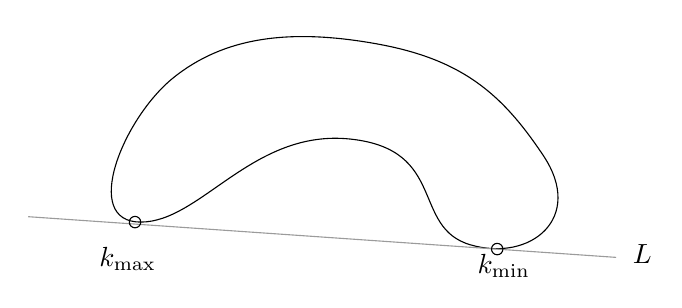
\begin{tikzpicture}[x=0.75pt,y=0.75pt,yscale=-1,xscale=1]
%uncomment if require: \path (0,300); %set diagram left start at 0, and has height of 300

%Shape: Polygon Curved [id:ds49662987101642475] 
\draw   (213,87) .. controls (237.2,67.6) and (268.4,63.2) .. (310.2,70.6) .. controls (352,78) and (371.2,94.6) .. (391.2,124.6) .. controls (411.2,154.6) and (385.13,175.92) .. (356.2,167.6) .. controls (327.27,159.28) and (345.2,121.6) .. (298.2,116.6) .. controls (251.2,111.6) and (226.2,156.6) .. (197.2,156.6) .. controls (168.2,156.6) and (188.8,106.4) .. (213,87) -- cycle ;
%Straight Lines [id:da34126944987507324] 
\draw [color={rgb, 255:red, 155; green, 155; blue, 155 }  ,draw opacity=1 ]   (143,154) -- (426.2,173.6) ;
%Shape: Circle [id:dp14005809041388972] 
\draw   (191.7,156.6) .. controls (191.7,155.08) and (192.93,153.85) .. (194.45,153.85) .. controls (195.97,153.85) and (197.2,155.08) .. (197.2,156.6) .. controls (197.2,158.12) and (195.97,159.35) .. (194.45,159.35) .. controls (192.93,159.35) and (191.7,158.12) .. (191.7,156.6) -- cycle ;
%Shape: Circle [id:dp3958585671594774] 
\draw   (366.2,169.6) .. controls (366.2,168.08) and (367.43,166.85) .. (368.95,166.85) .. controls (370.47,166.85) and (371.7,168.08) .. (371.7,169.6) .. controls (371.7,171.12) and (370.47,172.35) .. (368.95,172.35) .. controls (367.43,172.35) and (366.2,171.12) .. (366.2,169.6) -- cycle ;

% Text Node
\draw (358.2,171) node [anchor=north west][inner sep=0.75pt]    {$k_{\min}$};
% Text Node
\draw (176,167.4) node [anchor=north west][inner sep=0.75pt]    {$k_{\max}$};
% Text Node
\draw (433,166.4) node [anchor=north west][inner sep=0.75pt]    {$L$};


\end{tikzpicture}
\end{center}
(Reason: simple closed + convexity $\Rightarrow \theta(s)
$ is increasing on $[0,2\pi]$, the same argument as the previous page.) 
This implies that there must be points on both sides of $L$. 

\textbf{Claim }: No other points of $C$ meet $L$. 
\begin{center}
    


\tikzset{every picture/.style={line width=0.75pt}} %set default line width to 0.75pt        

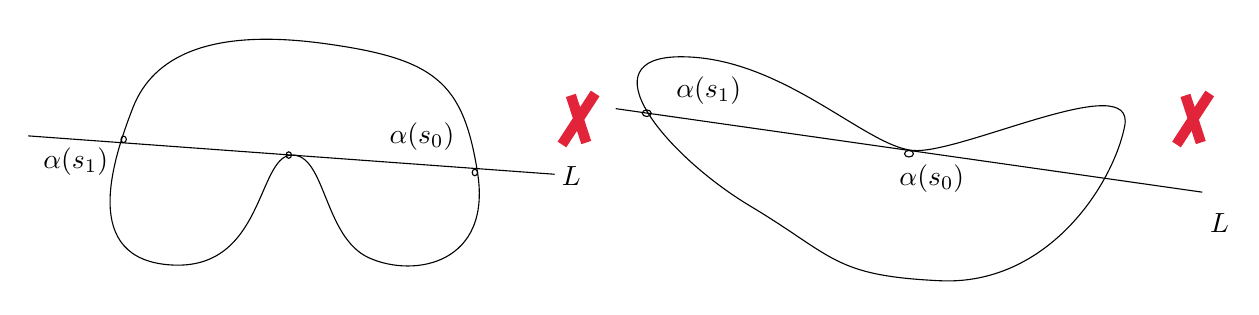
\begin{tikzpicture}[x=0.75pt,y=0.75pt,yscale=-0.9,xscale=0.9]
%uncomment if require: \path (0,300); %set diagram left start at 0, and has height of 300

%Shape: Polygon Curved [id:ds3071120878409017] 
\draw   (86.68,128.1) .. controls (97.49,100.08) and (128.53,85.42) .. (188.61,93.54) .. controls (248.68,101.67) and (263.51,114.09) .. (271.23,162.66) .. controls (278.95,211.23) and (237.88,219.31) .. (213.32,208.43) .. controls (188.76,197.55) and (189.99,152.5) .. (171.62,153.32) .. controls (153.25,154.14) and (156.95,214.97) .. (107.53,212.17) .. controls (58.11,209.36) and (75.87,156.12) .. (86.68,128.1) -- cycle ;
%Straight Lines [id:da6805550926024335] 
\draw    (30.7,143.05) -- (312.54,163.6) ;
%Shape: Ellipse [id:dp5838511313323707] 
\draw   (168.76,153.32) .. controls (168.76,154.28) and (169.4,155.05) .. (170.19,155.05) .. controls (170.98,155.05) and (171.62,154.28) .. (171.62,153.32) .. controls (171.62,152.37) and (170.98,151.59) .. (170.19,151.59) .. controls (169.4,151.59) and (168.76,152.37) .. (168.76,153.32) -- cycle ;
%Shape: Ellipse [id:dp38388215977449014] 
\draw   (80.35,144.92) .. controls (80.35,145.88) and (80.99,146.65) .. (81.78,146.65) .. controls (82.57,146.65) and (83.21,145.88) .. (83.21,144.92) .. controls (83.21,143.97) and (82.57,143.19) .. (81.78,143.19) .. controls (80.99,143.19) and (80.35,143.97) .. (80.35,144.92) -- cycle ;
%Shape: Ellipse [id:dp36329266716854014] 
\draw   (268.37,162.66) .. controls (268.37,163.62) and (269.01,164.39) .. (269.8,164.39) .. controls (270.59,164.39) and (271.23,163.62) .. (271.23,162.66) .. controls (271.23,161.71) and (270.59,160.93) .. (269.8,160.93) .. controls (269.01,160.93) and (268.37,161.71) .. (268.37,162.66) -- cycle ;
%Shape: Right Angle [id:dp5810238140777244] 
\draw  [color={rgb, 255:red, 226; green, 36; blue, 58 }  ,draw opacity=1 ][line width=3.75]  (321.19,121.39) -- (325.31,134.01) -- (316.42,147.66) ;
%Shape: Right Angle [id:dp947959045950229] 
\draw  [color={rgb, 255:red, 226; green, 36; blue, 58 }  ,draw opacity=1 ][line width=3.75]  (329.43,146.61) -- (325.31,133.99) -- (334.2,120.35) ;

%Shape: Polygon Curved [id:ds8274619497323568] 
\draw   (417.24,180.63) .. controls (371.98,153.54) and (327.65,100.02) .. (381.22,100.7) .. controls (434.78,101.37) and (478.59,148.3) .. (504.05,150.83) .. controls (529.51,153.35) and (624.11,106.12) .. (617.64,137.96) .. controls (611.18,169.79) and (576.08,223.31) .. (518.82,220.6) .. controls (461.56,217.89) and (462.49,207.73) .. (417.24,180.63) -- cycle ;
%Straight Lines [id:da11395275306166774] 
\draw    (345.2,128.47) -- (659.2,173.18) ;
%Shape: Ellipse [id:dp10283110241696836] 
\draw   (499.8,152.59) .. controls (499.8,151.61) and (500.87,150.83) .. (502.2,150.83) .. controls (503.53,150.83) and (504.6,151.61) .. (504.6,152.59) .. controls (504.6,153.56) and (503.53,154.35) .. (502.2,154.35) .. controls (500.87,154.35) and (499.8,153.56) .. (499.8,152.59) -- cycle ;
%Shape: Ellipse [id:dp5551670999500844] 
\draw   (359.42,130.91) .. controls (359.42,129.94) and (360.5,129.15) .. (361.82,129.15) .. controls (363.15,129.15) and (364.22,129.94) .. (364.22,130.91) .. controls (364.22,131.88) and (363.15,132.67) .. (361.82,132.67) .. controls (360.5,132.67) and (359.42,131.88) .. (359.42,130.91) -- cycle ;
%Shape: Right Angle [id:dp5407499071484163] 
\draw  [color={rgb, 255:red, 226; green, 36; blue, 58 }  ,draw opacity=1 ][line width=3.75]  (650.19,121.39) -- (654.31,134.01) -- (645.42,147.66) ;
%Shape: Right Angle [id:dp08794142716571418] 
\draw  [color={rgb, 255:red, 226; green, 36; blue, 58 }  ,draw opacity=1 ][line width=3.75]  (658.43,146.61) -- (654.31,133.99) -- (663.2,120.35) ;


% Text Node
\draw (37.41,147.77) node [anchor=north west][inner sep=0.75pt]    {$\alpha ( s_{1})$};
% Text Node
\draw (222.75,134.5) node [anchor=north west][inner sep=0.75pt]    {$\alpha ( s_{0})$};
% Text Node
\draw (315,158.05) node [anchor=north west][inner sep=0.75pt]    {$L$};
% Text Node
\draw (376.27,110) node [anchor=north west][inner sep=0.75pt]    {$\alpha ( s_{1})$};
% Text Node
\draw (495.71,157.24) node [anchor=north west][inner sep=0.75pt]    {$\alpha ( s_{0})$};
% Text Node
\draw (662,183.05) node [anchor=north west][inner sep=0.75pt]    {$L$};


\end{tikzpicture}
\end{center}
(Reason: same as Claim 1.) Hence, Claim 1 + Claim 2$\Rightarrow$ 
\begin{center}
    


\tikzset{every picture/.style={line width=0.75pt}} %set default line width to 0.75pt        

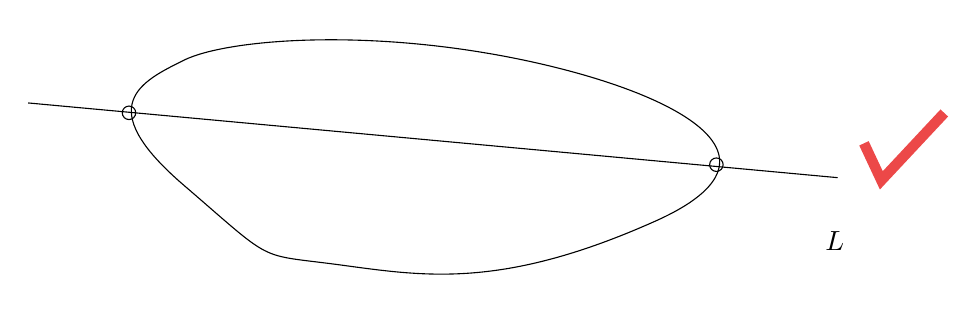
\begin{tikzpicture}[x=0.75pt,y=0.75pt,yscale=-1,xscale=1]
%uncomment if require: \path (0,300); %set diagram left start at 0, and has height of 300

%Shape: Polygon Curved [id:ds7702382474499099] 
\draw   (140,53) .. controls (160,43) and (225.2,37.5) .. (297.2,51.5) .. controls (369.2,65.5) and (441.2,97.5) .. (367.2,130.5) .. controls (293.2,163.5) and (255.95,156.97) .. (215.2,151.5) .. controls (174.45,146.03) and (184.8,151.5) .. (140,113) .. controls (95.2,74.5) and (120,63) .. (140,53) -- cycle ;
%Straight Lines [id:da6986447532784184] 
\draw    (65.2,73.5) -- (455.2,109.5) ;
%Shape: Circle [id:dp736182231164852] 
\draw   (393.5,103.25) .. controls (393.5,101.46) and (394.96,100) .. (396.75,100) .. controls (398.54,100) and (400,101.46) .. (400,103.25) .. controls (400,105.04) and (398.54,106.5) .. (396.75,106.5) .. controls (394.96,106.5) and (393.5,105.04) .. (393.5,103.25) -- cycle ;
%Shape: Circle [id:dp35739367600902905] 
\draw   (110.5,78.25) .. controls (110.5,76.46) and (111.96,75) .. (113.75,75) .. controls (115.54,75) and (117,76.46) .. (117,78.25) .. controls (117,80.04) and (115.54,81.5) .. (113.75,81.5) .. controls (111.96,81.5) and (110.5,80.04) .. (110.5,78.25) -- cycle ;
%Shape: Right Angle [id:dp7746325035072514] 
\draw  [color={rgb, 255:red, 236; green, 72; blue, 72 }  ,draw opacity=1 ][line width=3.75]  (506.56,78.34) -- (476.22,110.79) -- (467.86,92.95) ;

% Text Node
\draw (448,134.4) node [anchor=north west][inner sep=0.75pt]    {$L$};


\end{tikzpicture}
\end{center}
\textbf{Claim 3}: $\exists$ a third and a fourth vertex. (See the proof)

\begin{exercise}
    Let $\alpha(s)=\left(x(s),y(s)\right)$ be a simple closed curve in 
    $\mathbb{R}^2$. Let $\tilde{\alpha}(s)$ be the image of $\alpha(s)$ 
    under stereographic projection. Show that if $\alpha(s_0)$ is a vertex 
    of $\alpha(s)$, then $\tilde{\alpha}(s_0)$ has vanishing torsion.
\end{exercise}
\begin{example}
    \hfill
    \begin{itemize}
        \item The circle with radius $r$ and curvature $k=\frac{1}{r}$ has infinitely many vertices.
        \begin{center}
            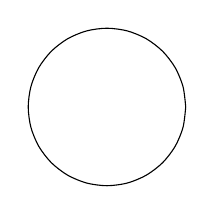
\begin{tikzpicture}
                \draw[smooth,domain=0:360,variable=\t]
                plot ({cos(\t)},{sin(\t)});
            \end{tikzpicture}
        \end{center}
        \item An ellipse has four vertices.
        \begin{center}
            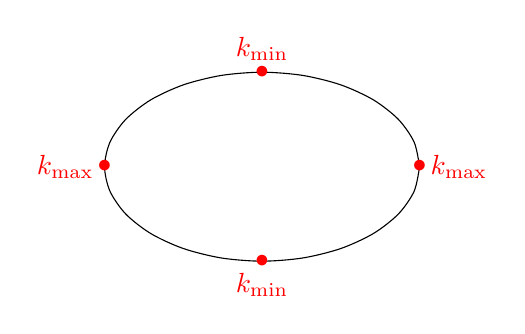
\begin{tikzpicture}
                \draw[smooth,domain=0:360,variable=\t]
                plot ({2*cos(\t)},{1.2*sin(\t)});
                \draw[red] (2,0) node {$\bullet$};
                \draw[red] (-2,0) node {$\bullet$};
                \draw[red] (0,1.2) node {$\bullet$};
                \draw[red] (0,-1.2) node {$\bullet$};
                \draw[red] (2.5,0) node {$k_{\max}$};
                \draw[red] (-2.5,0) node {$k_{\max}$};
                \draw[red] (0,1.5) node {$k_{\min}$};
                \draw[red] (0,-1.5) node {$k_{\min}$};
            \end{tikzpicture}
        \end{center}
        \item Although this is nonconvex, it has more than four vertices.
        \begin{center}
            


\tikzset{every picture/.style={line width=0.75pt}} %set default line width to 0.75pt        

\begin{tikzpicture}[x=0.75pt,y=0.75pt,yscale=-1,xscale=1]
%uncomment if require: \path (0,300); %set diagram left start at 0, and has height of 300

%Shape: Polygon Curved [id:ds4426374143902496] 
\draw   (276.2,124.7) .. controls (296.2,114.7) and (288,52.96) .. (296.2,52.7) .. controls (304.4,52.44) and (323.14,127.79) .. (353.2,126.7) .. controls (383.26,125.61) and (373.2,41.7) .. (383.2,44.7) .. controls (393.2,47.7) and (392.2,119.7) .. (436.2,133.7) .. controls (480.2,147.7) and (468.2,197.7) .. (449.2,216.7) .. controls (430.2,235.7) and (376.11,240.74) .. (353.2,239.7) .. controls (330.29,238.66) and (263.5,210.75) .. (251,192) .. controls (238.5,173.25) and (256.2,134.7) .. (276.2,124.7) -- cycle ;
%Shape: Circle [id:dp24475690948115414] 
\draw   (350.95,241.95) .. controls (350.95,240.71) and (351.96,239.7) .. (353.2,239.7) .. controls (354.44,239.7) and (355.45,240.71) .. (355.45,241.95) .. controls (355.45,243.19) and (354.44,244.2) .. (353.2,244.2) .. controls (351.96,244.2) and (350.95,243.19) .. (350.95,241.95) -- cycle ;
%Shape: Circle [id:dp6463699176238631] 
\draw   (293.95,52.7) .. controls (293.95,51.46) and (294.96,50.45) .. (296.2,50.45) .. controls (297.44,50.45) and (298.45,51.46) .. (298.45,52.7) .. controls (298.45,53.94) and (297.44,54.95) .. (296.2,54.95) .. controls (294.96,54.95) and (293.95,53.94) .. (293.95,52.7) -- cycle ;
%Shape: Circle [id:dp22246063551555872] 
\draw   (419.5,126.25) .. controls (419.5,125.01) and (420.51,124) .. (421.75,124) .. controls (422.99,124) and (424,125.01) .. (424,126.25) .. controls (424,127.49) and (422.99,128.5) .. (421.75,128.5) .. controls (420.51,128.5) and (419.5,127.49) .. (419.5,126.25) -- cycle ;
%Shape: Circle [id:dp15960337604147457] 
\draw   (350.95,126.7) .. controls (350.95,125.46) and (351.96,124.45) .. (353.2,124.45) .. controls (354.44,124.45) and (355.45,125.46) .. (355.45,126.7) .. controls (355.45,127.94) and (354.44,128.95) .. (353.2,128.95) .. controls (351.96,128.95) and (350.95,127.94) .. (350.95,126.7) -- cycle ;
%Shape: Circle [id:dp04023095022735057] 
\draw   (378.7,44.7) .. controls (378.7,43.46) and (379.71,42.45) .. (380.95,42.45) .. controls (382.19,42.45) and (383.2,43.46) .. (383.2,44.7) .. controls (383.2,45.94) and (382.19,46.95) .. (380.95,46.95) .. controls (379.71,46.95) and (378.7,45.94) .. (378.7,44.7) -- cycle ;
%Shape: Circle [id:dp5025388061962088] 
\draw   (276.2,124.7) .. controls (276.2,123.46) and (277.21,122.45) .. (278.45,122.45) .. controls (279.69,122.45) and (280.7,123.46) .. (280.7,124.7) .. controls (280.7,125.94) and (279.69,126.95) .. (278.45,126.95) .. controls (277.21,126.95) and (276.2,125.94) .. (276.2,124.7) -- cycle ;




\end{tikzpicture}
        \end{center}
    \end{itemize}
\end{example}
\begin{proof}[Proof of \cref{thm:four-vertex theorem}]
    Let $\alpha(s)$ be parametrized by arclength. First, since the curvature
    $k(s)$ is a continuous function on $I$, it must have maximum and 
    minimum, at which $k'(s)=0$, \ie\ $\alpha(s)$ has at least $2$ vertices.
    Let $\alpha(s_0)$ be a $k_{\min}$ point, $\alpha(s_1)$ be a $k_{\max}$ 
    point. Consider a line $l$ connecting $\alpha(s_0)$ and $\alpha(s_1)$. For convenience, we assume line $l$ coincides with $x$-axis.
    \begin{center}
        


\tikzset{every picture/.style={line width=0.75pt}} %set default line width to 0.75pt        

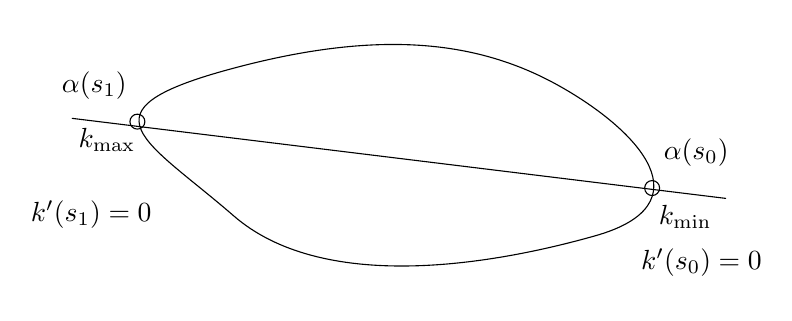
\begin{tikzpicture}[x=0.75pt,y=0.75pt,yscale=-1,xscale=1]
%uncomment if require: \path (0,300); %set diagram left start at 0, and has height of 300

%Shape: Polygon Curved [id:ds06277821638958292] 
\draw   (137.2,40.6) .. controls (210.2,20.6) and (258.2,26.6) .. (297.2,48.6) .. controls (336.2,70.6) and (367.2,105.6) .. (314.2,120.6) .. controls (261.2,135.6) and (182.2,147.6) .. (140,111) .. controls (97.8,74.4) and (64.2,60.6) .. (137.2,40.6) -- cycle ;
%Straight Lines [id:da7129598017341983] 
\draw    (62,64) -- (377.2,102.6) ;
%Shape: Circle [id:dp20289567099794015] 
\draw   (90,65.6) .. controls (90,63.61) and (91.61,62) .. (93.6,62) .. controls (95.59,62) and (97.2,63.61) .. (97.2,65.6) .. controls (97.2,67.59) and (95.59,69.2) .. (93.6,69.2) .. controls (91.61,69.2) and (90,67.59) .. (90,65.6) -- cycle ;
%Shape: Circle [id:dp11839975645101264] 
\draw   (338,97.6) .. controls (338,95.61) and (339.61,94) .. (341.6,94) .. controls (343.59,94) and (345.2,95.61) .. (345.2,97.6) .. controls (345.2,99.59) and (343.59,101.2) .. (341.6,101.2) .. controls (339.61,101.2) and (338,99.59) .. (338,97.6) -- cycle ;

% Text Node
\draw (56,40.4) node [anchor=north west][inner sep=0.75pt]    {$\alpha ( s_{1})$};
% Text Node
\draw (346,72.4) node [anchor=north west][inner sep=0.75pt]    {$\alpha ( s_{0})$};
% Text Node
\draw (64,67.4) node [anchor=north west][inner sep=0.75pt]    {$k_{\max}$};
% Text Node
\draw (343.6,104.6) node [anchor=north west][inner sep=0.75pt]    {$k_{\min}$};
% Text Node
\draw (41,102.4) node [anchor=north west][inner sep=0.75pt]    {$k'( s_{1}) =0$};
% Text Node
\draw (335,125.4) node [anchor=north west][inner sep=0.75pt]    {$k'( s_{0}) =0$};


\end{tikzpicture}
    \end{center}

    The First observation is: on $l$, there is no other point of $\alpha(s)$. 
    Hence, $\alpha(s)$ is divided into two pieces. If not, assume 
    $\alpha(s_2)$ is a third point, and W.L.O.G. assume $k'(s_2)=0$. 
    The tangent line at $\alpha(s_2)$ must be the same as $l$. Since the 
    curve $\alpha$ is convex, the whole curve $\alpha(s)$ must lie on the 
    same side of $l$. This forces the tangent lines of $\alpha(s_0)$ and 
    $\alpha(s_1)$ can only be $l$. But $\alpha(s_0)$ is a $k_{\min}$ point
    and $\alpha(s_1)$ is a $k_{\max}$ point, which implies $k(s_0)=k(s_1)=0$. Therefore, $k\equiv 0$ on $\alpha$, a contradiction.

    \begin{center}
        


\tikzset{every picture/.style={line width=0.75pt}} %set default line width to 0.75pt        

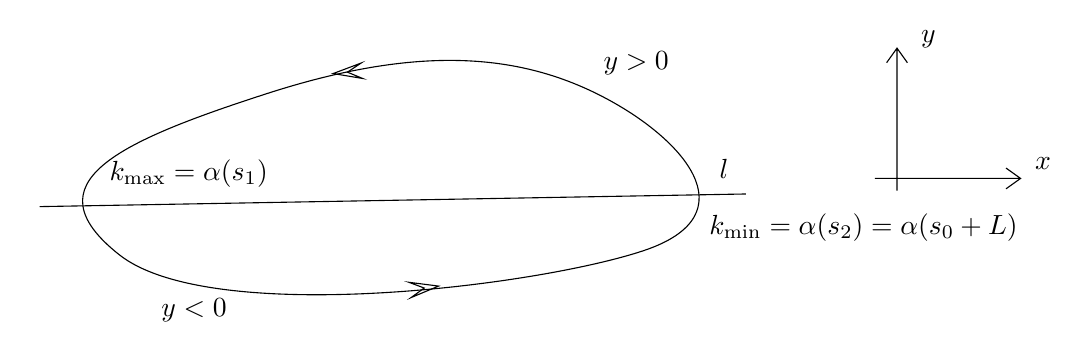
\begin{tikzpicture}[x=0.75pt,y=0.75pt,yscale=-1,xscale=1]
%uncomment if require: \path (0,300); %set diagram left start at 0, and has height of 300

%Shape: Polygon Curved [id:ds06277821638958292] 
\draw   (135.27,41.84) .. controls (207.3,18.59) and (255.52,22.43) .. (295.47,42.66) .. controls (335.42,62.89) and (368.74,100.23) .. (316.47,117.6) .. controls (264.19,134.96) and (107.7,154.16) .. (63.9,119.49) .. controls (20.1,84.82) and (63.24,65.1) .. (135.27,41.84) -- cycle ;
%Straight Lines [id:da7129598017341983] 
\draw    (25.55,96.35) -- (365.86,90.26) ;
\draw   (181.2,34.6) -- (166.97,32.25) -- (180.47,27.18) -- (173.9,31.57) -- cycle ;
\draw   (203.5,132.81) -- (217.81,134.63) -- (204.51,140.2) -- (210.9,135.57) -- cycle ;
%Shape: Axis 2D [id:dp6987088884625297] 
\draw  (428,82.77) -- (498.2,82.77)(438.67,20) -- (438.67,88.6) (491.2,77.77) -- (498.2,82.77) -- (491.2,87.77) (433.67,27) -- (438.67,20) -- (443.67,27)  ;

% Text Node
\draw (296,20.4) node [anchor=north west][inner sep=0.75pt]    {$y >0$};
% Text Node
\draw (83,139.4) node [anchor=north west][inner sep=0.75pt]    {$y< 0$};
% Text Node
\draw (347,98.4) node [anchor=north west][inner sep=0.75pt]    {$k_{\min} =\alpha ( s_{2}) =\alpha ( s_{0} +L)$};
% Text Node
\draw (58,72.4) node [anchor=north west][inner sep=0.75pt]    {$k_{\max} =\alpha ( s_{1})$};
% Text Node
\draw (504,71.4) node [anchor=north west][inner sep=0.75pt]    {$x$};
% Text Node
\draw (449,10.4) node [anchor=north west][inner sep=0.75pt]    {$y$};
% Text Node
\draw (352,72.4) node [anchor=north west][inner sep=0.75pt]    {$l$};


\end{tikzpicture}
    \end{center}

    Next, we look for the third vertex. If $\alpha(s)$ has only two vertices
    at $\alpha(s_0)$ and $\alpha(s_1)$, then from $s_0$ to $s_1$, $k'(s)>0$ 
    and from $s_1$ to $s_0+L$, $k'(s)<0$
    \[\Rightarrow y\cdot k'(s)\ge 0,~\forall s\]
    \[\Rightarrow 0<\int_\alpha y\cdot k'(s)\dd s=-\int_\alpha y'(s)k\dd s.\]
    Note that if 
    \[\alpha(s)=\left(x(s),y(s)\right), t(s)=\alpha'(s)\left(x'(s),y'(s)\right).\]
    \[t'(s)=\left(x''(s),y''(s)\right)=k \vec{n}=k(-y',x')\Rightarrow -k'(s)k=x''\]
    \[\therefore \int_\alpha y' k\dd s=\int_\alpha x'' \dd s=0.\]
    A contradiction!. Hence, there must be a third vertex, say $\alpha(s_2)$, at which $k'(s_2)=0$.

    Note that $k'(s)$ changes its sign at vertices, so the number of 
    vertices must be even. Then there are at least $4$ vertices.
\end{proof}
\begin{remark}
    The proof of the four-vertex theorem for non-convex 
    case can be found in Montiel-Ros's book Chapter 9.6. 
    (4-vertex theorem for space curves: simple closed curve on a convex surface has at least four points with vanishing torsion.)
\end{remark}
\subsection{Minkowski problem(1-d)}
\begin{theorem}[1-d Minkowski problem]
    \label{thm: Minkowski problem}
    Given a periodic, strictly positive function k, there is an oval in 
    $\mathbb{R}^2$ (\ie\ simple closed strictly convex curve) such that 
    the curvature function is $k$. 
\end{theorem}
\begin{definition}
    A plane curve $\alpha(t)$ is strictly convex iff $\alpha(t)$ is convex 
    and at each point, the tangent line meets with $\alpha(t)$ at only 
    one point.
\end{definition}
\begin{proposition}
    A simple closed curve is strictly convex iff with inward unit normal 
    vector field, the curvature function $k>0$. 
\end{proposition}
\textbf{Minkowski problem}: Given a strictly positive, periodic function
$k$, does there exist a simple closed convex curve $\alpha$ with $k$
as the curvature function?
\begin{remark}
    This is a prescribed curvature problem. There are a lot of similar 
    questions in geometry. Such problems are usually related to solving
    certain P.D.E.
\end{remark}
Let's derive a differential equation for the above problem. Let $\alpha$ be 
a strictly convex curve, then $k>0$, and we can use the angle parameter $\theta$, \ie\ 
\[\frac{\dd\theta}{\dd s}=k,~\frac{\dd s}{\dd \theta}=\frac{1}{k} \]
\begin{center}
    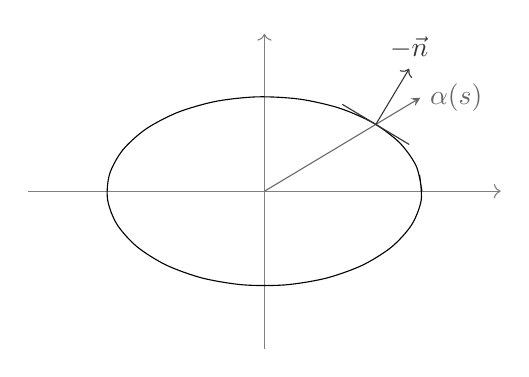
\begin{tikzpicture}
        \draw[black!50, thin, ->] (0, -2) -- (0, 2) ;
        \draw[black!50, thin, ->] (-3, 0) -- (3, 0) ;
        \draw[smooth,domain=0:370,variable=\t]
        plot ({2*cos(\t)},{1.2*sin(\t)});
        \draw[->,>=stealth,black!60](0,0)to({1.4*2*cos(45)},{1.4*1.2*sin(45)}) node[right]{$\alpha(s)$};
        \draw[smooth,domain=-0.3:0.3,variable=\t,black!80]
        plot ({2*cos(45)+2*(-sin(45))*\t},{1.2*sin(45)+1.2*cos(45)*\t});
        \draw[smooth,domain=0:0.5,variable=\t,black!80,->]
        plot ({2*cos(45)+1.2*cos(45)*\t},{1.2*sin(45)+2*(sin(45))*\t})
        node[above] {$-\vec{n}$};
    \end{tikzpicture}
\end{center}
Consider a function
\[
    h(s)=-\left<\alpha(s),\vec{n}(s)\right>\text{ support function}.
\]
(Recall $\int_C h(s)\dd s=2\cdot\mathrm{Area}$).\\
Clearly $h(0)=h(2\pi)$ if
 we use 
 $h(\theta)=-\langle\alpha\left(s(\theta)\right),\vec{n}\left(s(\theta)\right)\rangle$. 
 \begin{align*}
    h'(\theta)&=-\langle \alpha'(s)\frac{\dd s}{\dd\theta},\vec{n}(s)\rangle
    -\langle \alpha(\theta),\frac{\dd \vec{n}}{\dd s}\frac{\dd s}{\dd \theta}\rangle\\
    &=-\langle \alpha(\theta),-k\cdot\vec{t}\cdot\frac{1}{k}\rangle =\langle\alpha(\theta),\vec{t}\left(s(\theta)\right)\rangle
.\end{align*}
Hence, $h'(0)=h'(2\pi)$.

We also conclude that
\begin{align*}
    \alpha(\theta)&=\langle \alpha(\theta), \vec{t}\rangle \cdot \vec{t}
    +\langle \alpha(\theta), \vec{n}\rangle \cdot \vec{n}\\
    &=h'(\theta)\vec{t}-h(\theta)\vec{n}
,\end{align*}
\ie\ the curve is determined by the support function $h$. \\
$\left(\alpha(s)=h'(s)\dfrac{\dd s}{\dd \theta}\vec{t}-h(s)\vec{n}=h'(s)\dfrac{1}{k}\vec{t}-h(s)\vec{n}\right)$
\begin{align*}
    h''(\theta)&=\langle \alpha'(s)\frac{\dd s}{\dd \theta},\vec{t}\rangle
    +\langle \alpha(\theta),\frac{\dd \vec{t}}{\dd s}\frac{\dd s}{\dd \theta}
    \rangle\\
    &=\frac{1}{k}+\langle\alpha(\theta),k\vec{n}\cdot \frac{1}{k}\rangle=\frac{1}{k}-h
.\end{align*}
\ie\ $\boxed{h''(\theta)+h(\theta)=\frac{1}{k}}$.

Hence, if $\alpha(s)=\alpha(\theta)$ is a strictly convex closed curve, the
support function $h(\theta)=-\langle\alpha,\vec{n}\rangle$ satisfies a second
linear o.d.e.
\[h''(\theta)+h=\frac{1}{k}.\]
\textbf{Observation:} If $\exists~h$ that satisfies the equation above.
Note $\theta\in [0,2\pi)$, then
\begin{align*}
    \int_0^{2\pi}\cos\theta\frac{1}{k}\dd \theta&=
    \int_0^{2\pi} \cos\theta\cdot\left(h''\theta+h\right)\dd \theta\\
    &=\int_0^{2\pi}\sin\theta\cdot h'(\theta)+\int_0^{2\pi}\cos \theta \cdot h\\
    &=-\int_0^{2\pi}\cos\theta \cdot h(\theta)+\int_0^{2\pi}\cos\theta \cdot h=0
.\end{align*}
Similarly,
\[\int_0^{2\pi}\sin\theta\cdot\frac{1}{k}\dd \theta=0,\]
\ie\ if $k$ is the curvature of a strictly convex curve, it must satisfy
\[
    \int_0^{2\pi}\cos\theta\cdot\frac{1}{k}\dd \theta
    =\int_0^{2\pi}\sin\theta\cdot\frac{1}{k}\dd \theta
    =0
.\]

In fact, from o.d.e, we can directly construct the solution like this:
\[
    h(\theta)=-\cos\theta \int_0^\theta \frac{\sin \psi}{k}\dd \psi
    +\sin\theta \int_0^\theta \frac{\cos \psi}{k}\dd \psi  
.\]
Recall that $\vec{t}(s)=(\cos\theta,\sin\theta),~\vec{n}(s)=(-\sin \theta,\cos\theta).$
Since
\begin{align*}
    \alpha(\theta)&=h'(\theta)\vec{t}-h(\theta)\vec{n}\\
    &=\left(
        \cos\theta\sin\theta\int_0^\theta\frac{\sin\psi}{k}
        +\cos^2\theta\int_0^\theta\frac{\cos\psi}{k},
        \sin^2\theta\int_0^\theta\frac{\sin\psi}{k}
        +\sin\theta\cos\theta\int_0^\theta\frac{\cos\psi}{k}
    \right)\\
    &\quad-\left( 
        \sin\theta\cos\theta\int_0^\theta\frac{\sin\psi}{k}
        -\sin^2\theta\int_0^\theta\frac{\cos\psi}{k},
        -\cos^2\theta\int_0^\theta\frac{\sin\psi}{k}
        +\sin\theta\cos\theta\int_0^\theta\frac{\cos\psi}{k}
    \right)\\
    &=\left(
        \int_0^\theta\frac{\cos\psi}{k},
        \int_0^\theta\frac{\sin\psi}{k}
    \right)
\end{align*}
$\alpha(s)$ is closed $\Leftrightarrow~h(0)=h(2\pi),~h'(0)=h'(2\pi)
\Leftrightarrow \int_0^{2\pi}\cos\theta\cdot\dfrac{1}{k}\dd \theta
=\int_0^{2\pi}\sin\theta\cdot\dfrac{1}{k}\dd \theta
=0$.
\begin{remark}
    In general (higher dimensional case) solving a similar P.D.E. equation is highly nontrivial!
    
    Cheng-Yau 1976 CPAM: given a $C^{k,\alpha}$ positive function $k$ on the
    sphere $\mathbb{S}^n$ ($k\ge 3$), there is a strictly convex closed 
    hypersurface $M^n \hookrightarrow \mathbb{R}^{n+1}$ such
    that the Gaussian curvature is $k$.
\end{remark} 


\chapter{Differential Geometry of Surfaces}
\section*{A First Look}
\begin{figure}[htp]
\centering
\begin{subfigure}{0.3\textwidth}
    \centering
    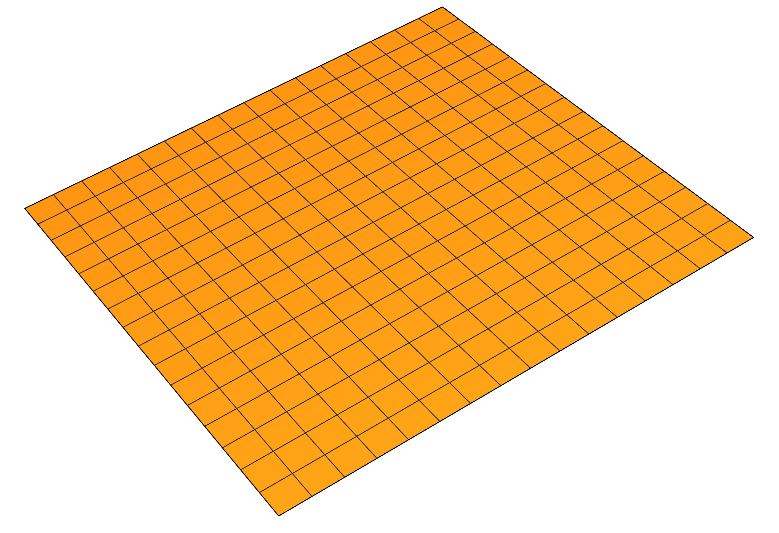
\includegraphics[width=\textwidth]{picture/week4/plane.pdf}
    \caption{Plane}
\end{subfigure}
\begin{subfigure}{0.2\textwidth}
    \centering
    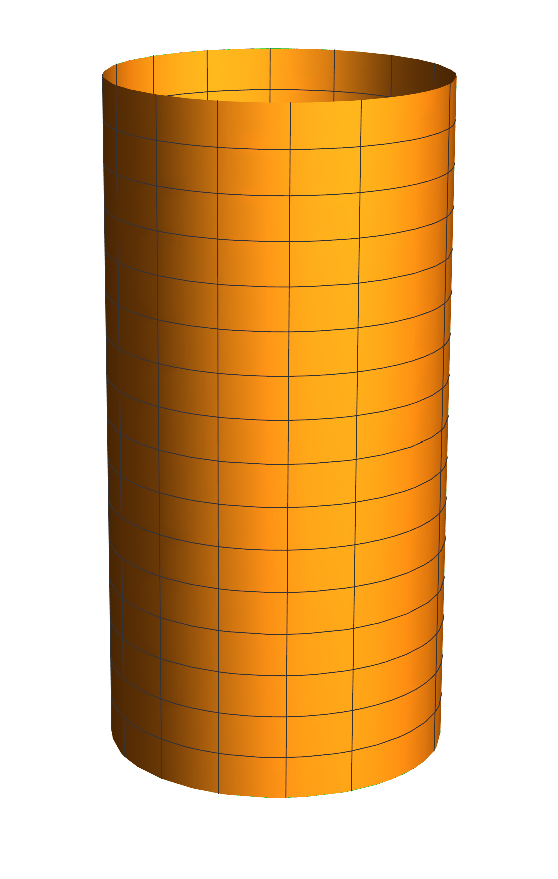
\includegraphics[width=\textwidth]{picture/week4/cylinder.pdf}
    \caption{Cylinder}
\end{subfigure}
\begin{subfigure}{0.4\textwidth}
    \centering
    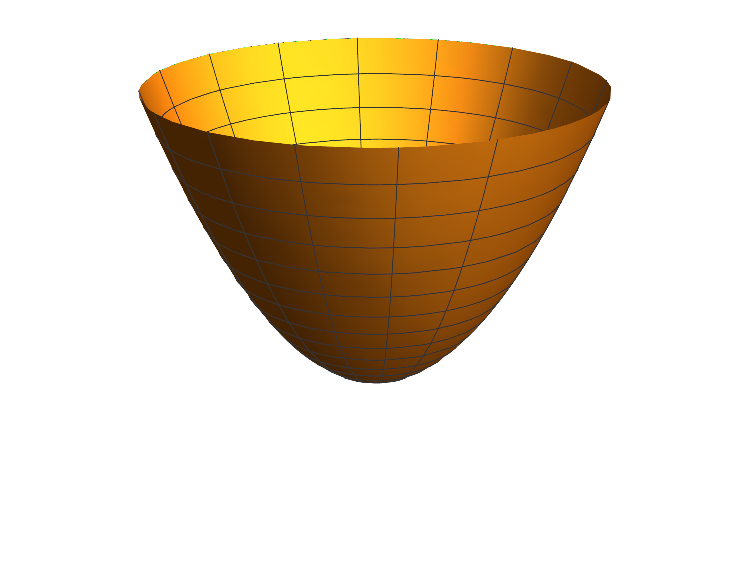
\includegraphics[width=\textwidth]{picture/week4/paraboloid.pdf}
    \caption{Paraboloid}
\end{subfigure}
\begin{subfigure}{0.3\textwidth}
    \centering
    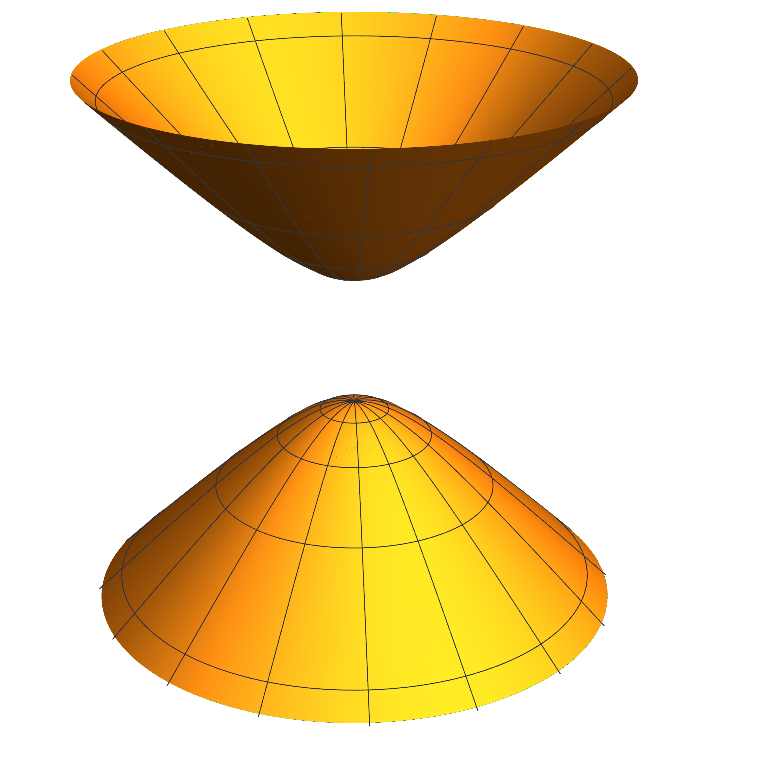
\includegraphics[width=\textwidth]{picture/week4/hyperboloid.pdf}
    \caption{Hyperboloid}
\end{subfigure}
\begin{subfigure}{0.2\textwidth}
    \centering
    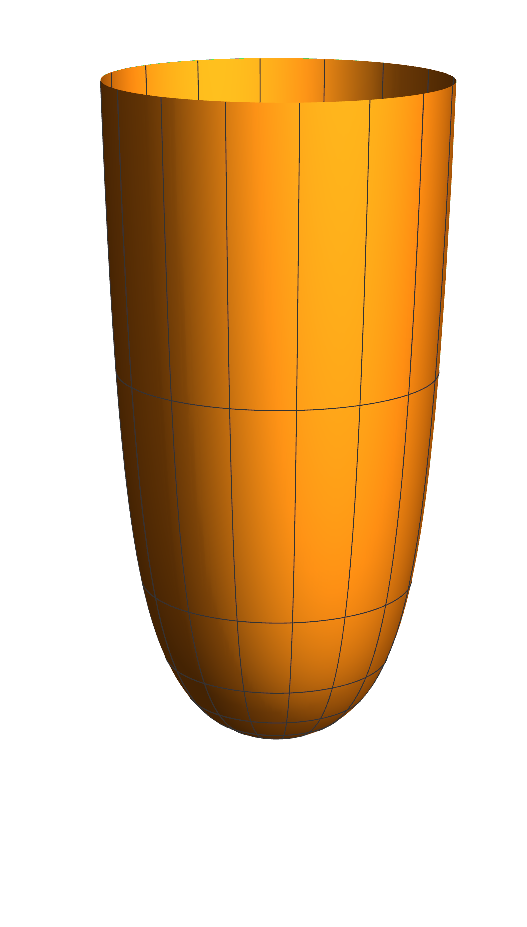
\includegraphics[width=\textwidth]{picture/week4/cigar.pdf}
    \caption{Cigar soliton}
\end{subfigure}
\caption*{Surface collection 1}
\end{figure}

\begin{figure}
\centering
\begin{subfigure}{0.25\textwidth}
    \centering
    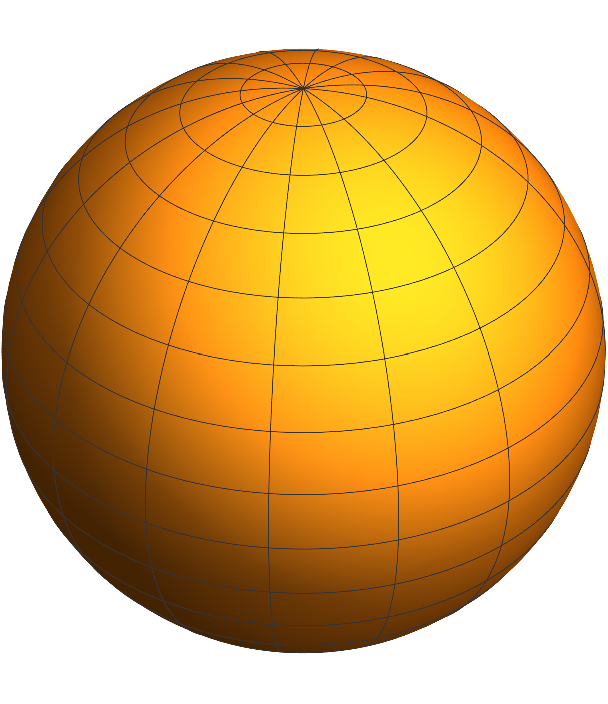
\includegraphics[width=\textwidth]{picture/week4/sphere.pdf}
    \caption{\(\mathbb{S}^2\)}
\end{subfigure}
\begin{subfigure}{0.35\textwidth}
    \centering
    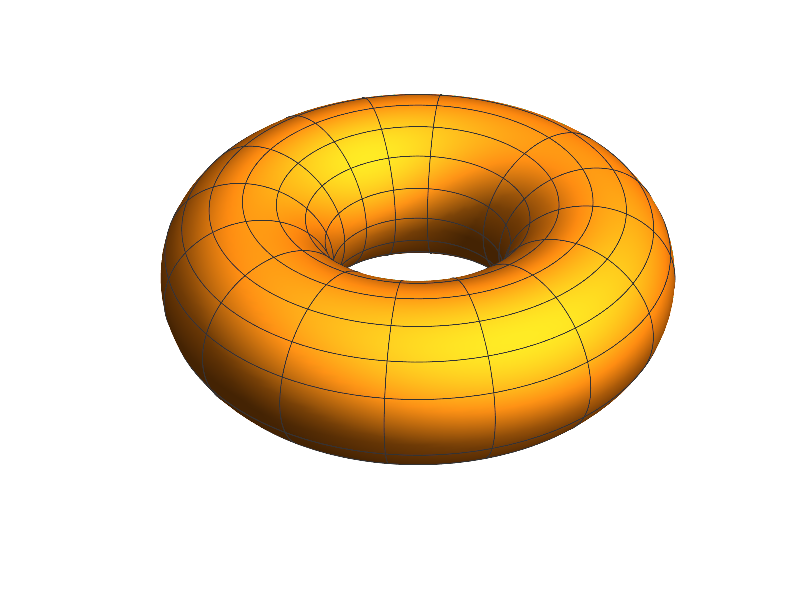
\includegraphics[width=\textwidth]{picture/week4/torus.pdf}
    \caption{\(\mathbb{T}^2\)}
\end{subfigure}
\begin{subfigure}{0.35\textwidth}
    \centering
    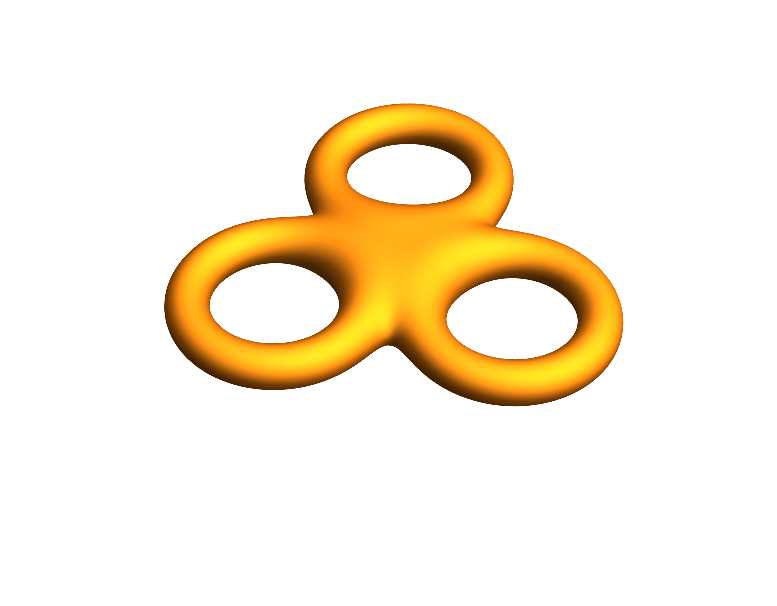
\includegraphics[width=\textwidth]{picture/week4/torus3.pdf}
    \caption{\(\Sigma_g\) for \(g=3\)}
\end{subfigure}
\caption*{Surface collection 2}
\end{figure}

\begin{figure}
\centering
\begin{subfigure}{0.45\textwidth}
    \centering
    
\includegraphics[width=\textwidth]{picture/week4/helicoid.pdf}
    \caption{Helicoid}
\end{subfigure}
\begin{subfigure}{0.45\textwidth}
    \centering
    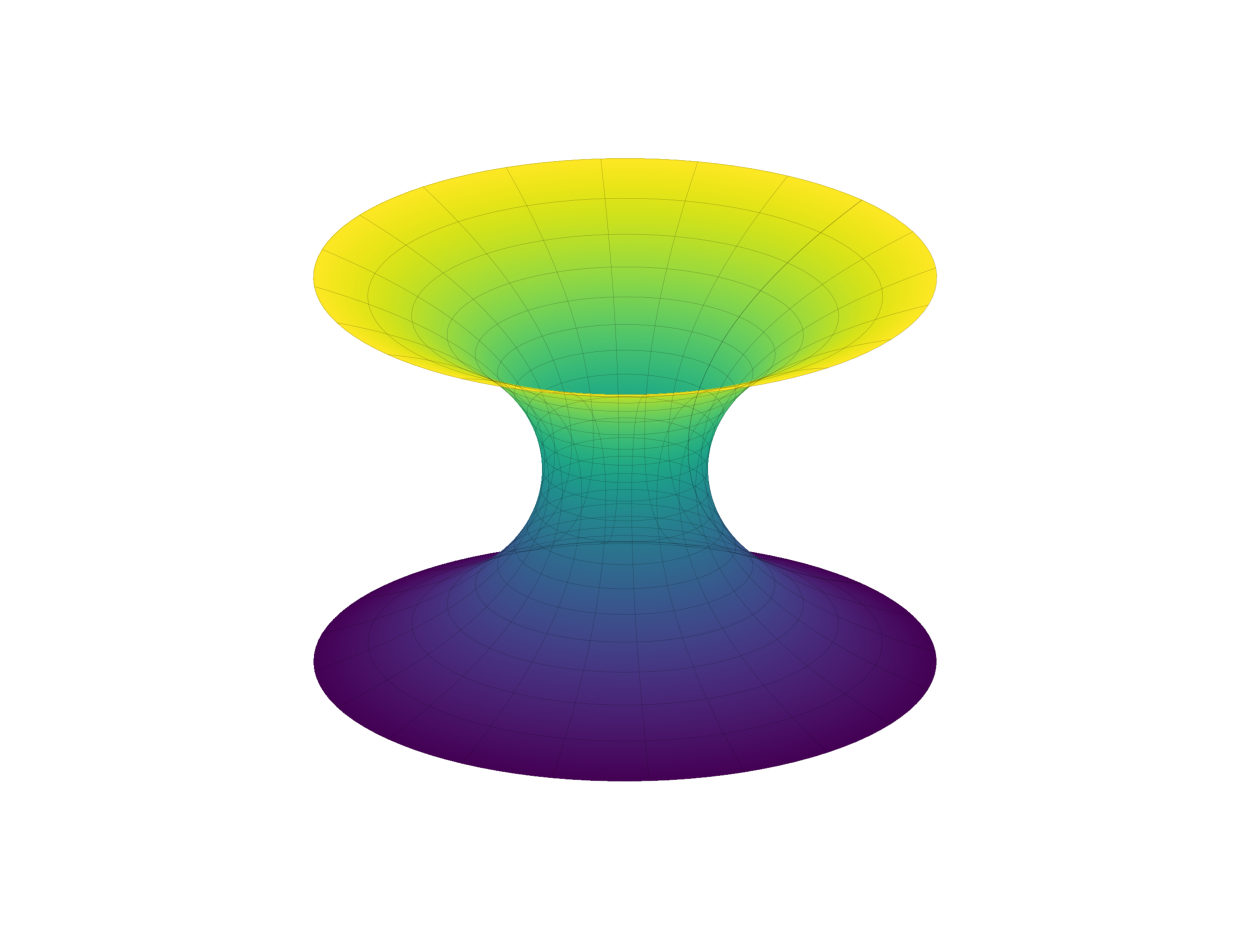
\includegraphics[width=\textwidth]{picture/week4/catenoid.pdf}
    \caption{Catenoid}
\end{subfigure}
\begin{subfigure}{0.5\textwidth}
    \centering
    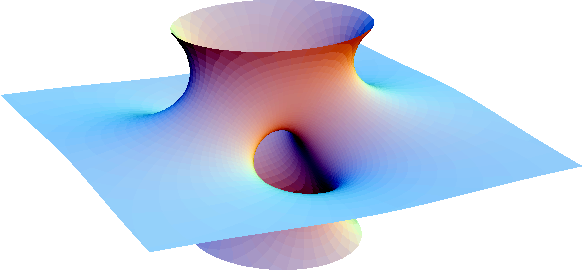
\includegraphics[width=\textwidth]{picture/week4/costa.pdf}
    \caption{Costa minimal surface}
\end{subfigure}
\begin{subfigure}{0.4\textwidth}
    \centering
    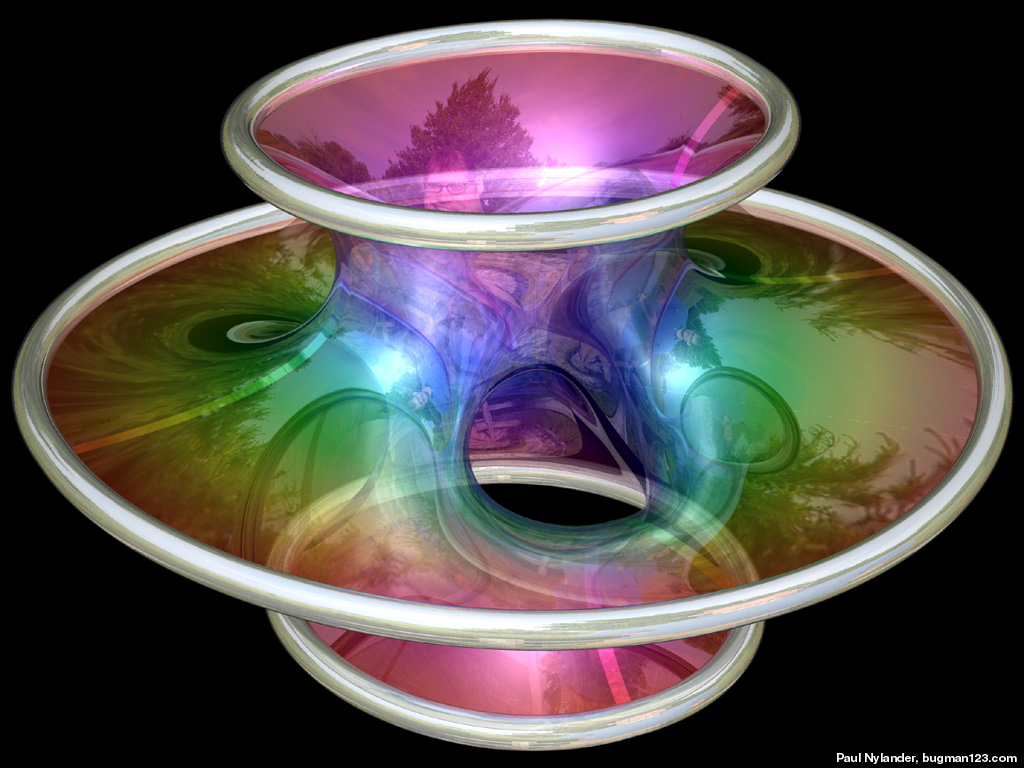
\includegraphics[width=\textwidth]{picture/week4/Costa-large.jpg}
    \caption{Soap bubble}
\end{subfigure}
\caption*{Surface collection 3}
\end{figure}

\begin{figure}
\centering
\begin{subfigure}{0.3\textwidth}
    \centering
    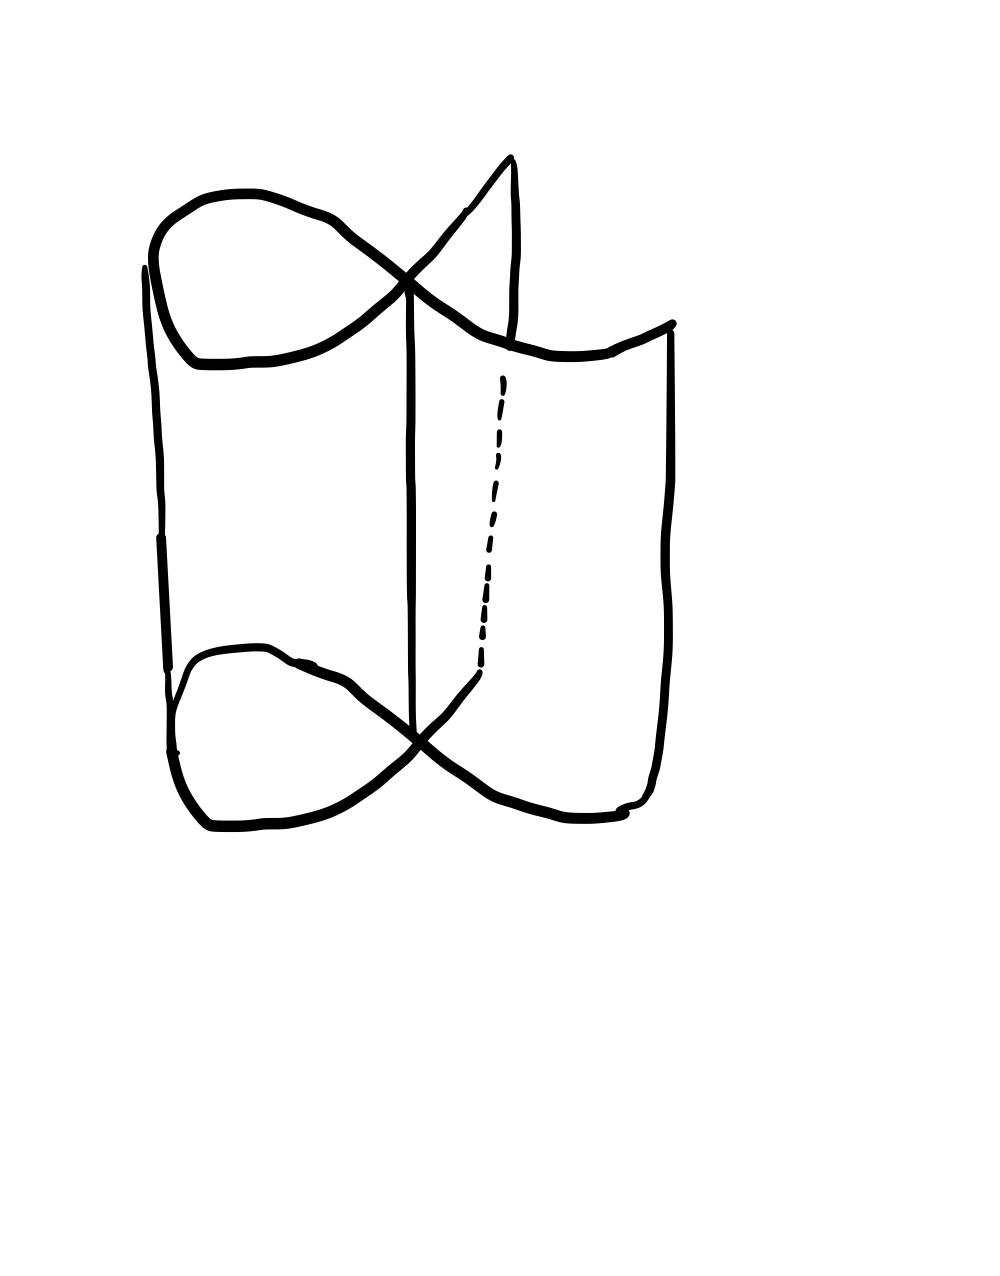
\includegraphics[width=\textwidth]{picture/week4/self-intersetcion.png}
    \caption{Self-intersected}
\end{subfigure}
\begin{subfigure}{0.35\textwidth}
    \centering
    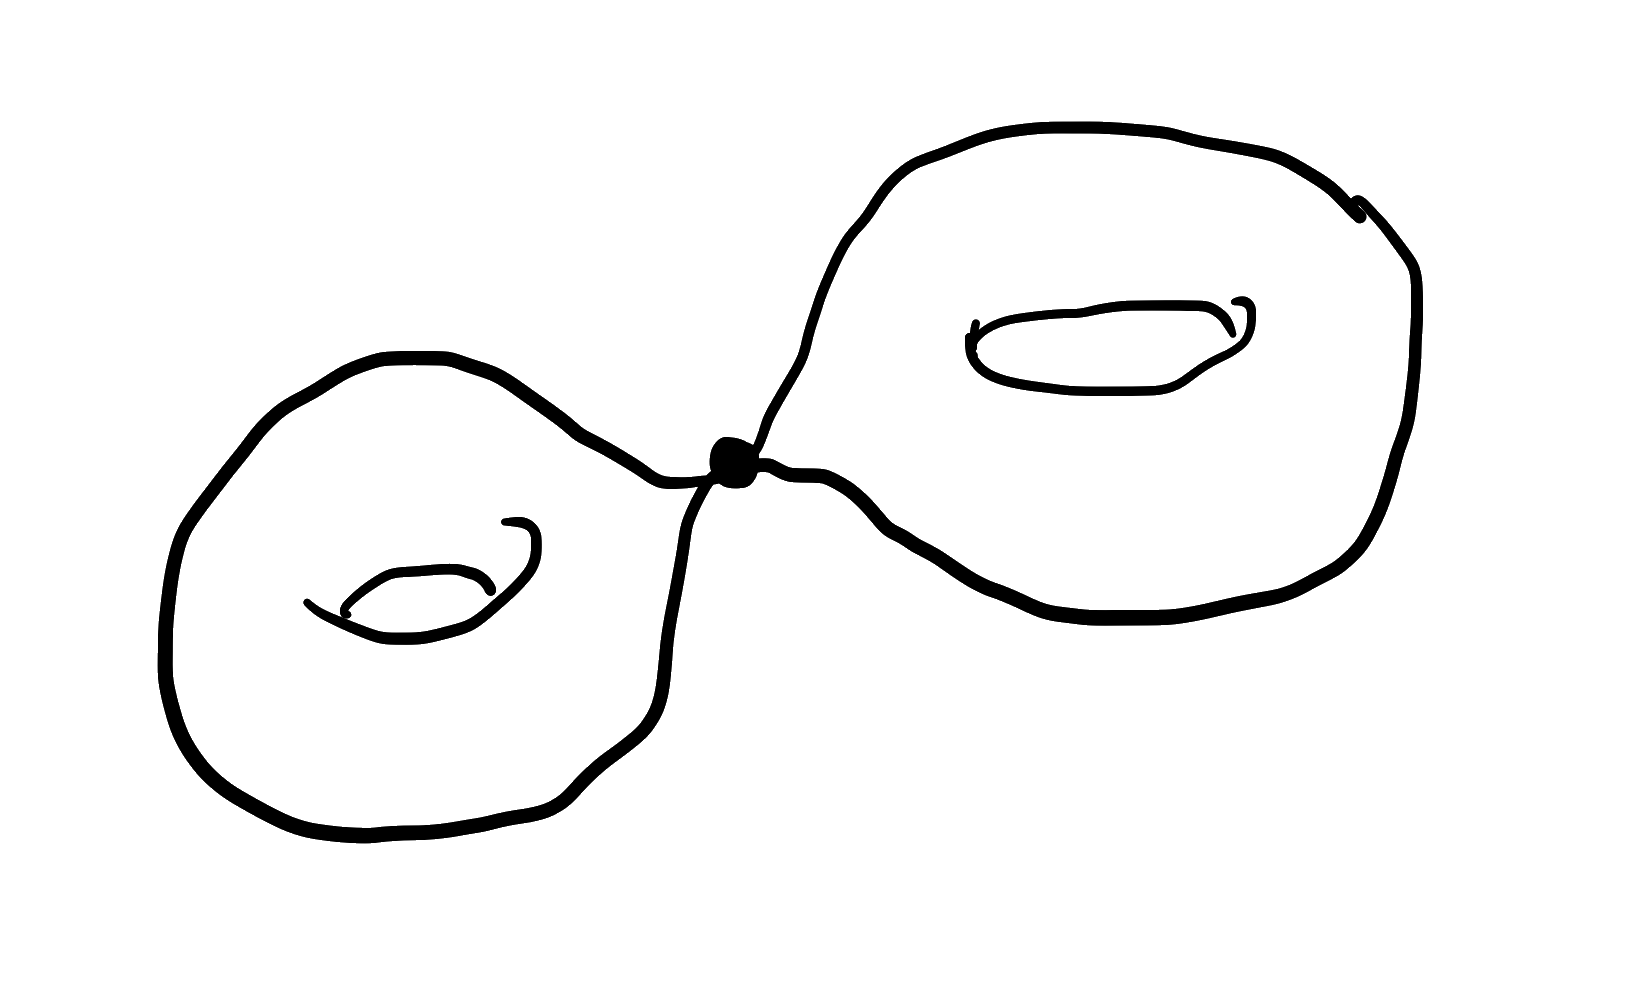
\includegraphics[width=\textwidth]{picture/week4/node.png}
    \caption{Nodal surfaces}
\end{subfigure}
\begin{subfigure}{0.3\textwidth}
    \centering
    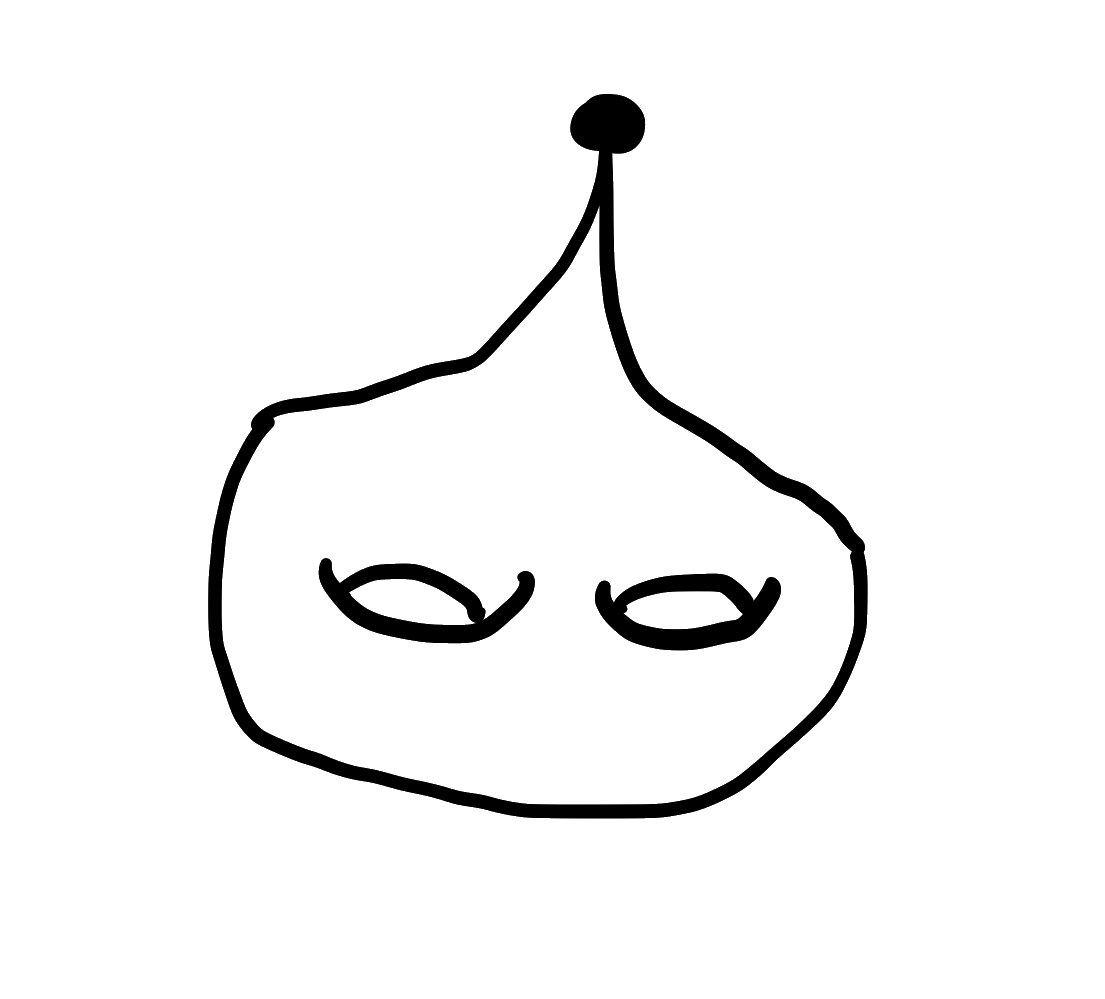
\includegraphics[width=\textwidth]{picture/week4/cusp.png}
    \caption{Cusp}
\end{subfigure}
\caption*{``Surface'' collection 4}
\end{figure}

\begin{example}\hfill
\begin{itemize}
    \item Collection 1 are complete non-compact surfaces.
    \item Collection 2 are compact surfaces without boundary (closed).
    \item Collection 3 are so called minimal surfaces, a very important class
        of surfaces. The term ``minimal'' intuits smallest area in certain sense.
    \item There are surfaces will NOT be investigated in this course, the ones with
        self-intersection, node points or cusps, and non-orientable surfaces.
\end{itemize}    
\end{example}

\section{Definition of Regular Surface}

\begin{definition}[Regular surfaces in \(\mathbb{R}^3\)]\hfill\par
    A subset \(S\subset \mathbb{R}^3\) is called a regular surface, if \(\forall\,p
    \in S\), \(\exists\, V\subset\mathbb{R}^3\) neighborhood of \(p\), an open set
    \(U\subset \mathbb{R}^2\) and a trivialization map \[
        F\colon U\to V\cap S
    .\] \st\ \(F\) is smooth, homeomorphism onto its image, and regular.
\end{definition}
\begin{remark}\hfill
\begin{enumerate}[(1)]
    \item \(F\) is homeomorphism means both \(F\) and \(F^{-1}\) are continuous map.
    \item \(F\) is ``regular'' means \(\forall\,p\in U\), \(\dif F_p\) is an 
        injection as linear map \(\mathbb{R}^2\to \mathbb{R}^3\).
\end{enumerate}
\end{remark}

Let's see what the term ``regular'' means:

Assume \(F\) is written as \(F(u,v)=(x(u,v),y(u,v),z(u,v))\), at \(p\in U\), \[
    \dd{F_p}\colon T_p U\to T_{F(p)}S
\] is a linear map. On \(\mathbb{R}^2\), coordinate vector fields \(\{\pdv{u},
\pdv{v}\}\) form a basis. On \(\mathbb{R}^3\) we also have standard basis
\(\{\pdv{x},\pdv{y},\pdv{z}\}\). Then \[
    \dd{F_p}\begin{bmatrix}
        \pdv{u}\\ \pdv{v}
    \end{bmatrix}
    =\begin{bmatrix}
        \pdv{x}{u} & \pdv{y}{u} & \pdv{z}{u} \\ 
        \pdv{x}{v} & \pdv{y}{v} & \pdv{z}{v}
    \end{bmatrix}
    \begin{bmatrix}
        \pdv{x}\\ \pdv{y}\\ \pdv{z}
    \end{bmatrix}
.\] Hence
\begin{align*}
    \dd{F_p}\text{ is injective}
    \iff & \ker\dd{F_p}=0 \\
    \iff & \pdv{(x,y,z)}{(u,v)}\text{ has rank 2} \\
    \iff & \pdv{F}{u}\text{ \& }\pdv{F}{v}\text{ are linearly independent} \\
    \iff & \pdv{F}{u}\times \pdv{F}{v}\neq 0. \\
    & \text{\small\itshape\/ (Geometrically this defines the normal vector field} \\
    & \text{\small\itshape\/ of the tangent plane)} \\
    \iff & \text{ One of the following minors is non-zero:}\\
    & \quad\left|\pdv{(x,y)}{(u,v)}\right|,\quad\left|\pdv{(x,z)}{(u,v)}\right|,
    \quad\left|\pdv{(y,z)}{(u,v)}\right|
\end{align*}
{\small\itshape
    (Geometrically, this means \((u,v)\) can be viewed as coordinate at \(p\in S\)
    via \(F\). In fact, since ``\(\dd{F_p}\) is injective'' is an open condition,
    \((u,v)\) serves as a local coordinate chart in a neighborhood of \(p\))
}

We also call \(F\) to be a local parametrization of \(S\). Note that such \(F\)
is usually not globally defined.

From the definition, we see a regular surface in \(\mathbb{R}^3\) is characterized
by at each point, we can find a ``smooth'' slice chart in a neighbourhood of the
point. The term ``slice chart'' means coordinate chart with local part of the
surface containing in the chart as a slice.

\begin{question}
    Consider two points \(p,q\) on the surface, live close to each other. It might
    happen that their corresponding coordinate chart overlap. Then in the
    intersection of two charts, there are two different parametrizations. What
    relation between these two parametrizations should be?
\end{question}
% Figure here

Set-up: \(F_1\colon U_1\to V_1\cap S,\ (u,v)\mapsto F_1(u,v)\),\hfill \(F_2\colon
U_2\to V_2\cap S,\ (\alpha,\beta)\mapsto F_2(\alpha,\beta)\)

Let \(W=V_1\cap V_2\cap S\), since \(F_i\) is homeomorphism, \(F_1^{-1}(W)\subset U,
\ F_2^{-1}(W)\subset U_2\).

\noindent\underline{\textbf{Claim:}} (Very important).\par
\(G=F_2^{-1}\circ F_1\colon F_1^{-1}(W)\to F_2^{-1}(W)\) is a diffeomorphism,\ie\ 
both \(G\) and \(G^{-1}\) are smooth functions.

The importance of this claim leads us to give an intrinsic definition of a regular
surface \(S\). \ie\ a regular surface is obtained by padding up open sets in
\(\mathbb{R}^2\), in a smooth way. Later in differential geometry course, we'll
define a smooth manifold by such intrinsic definition. The diffeomorphism \(G\)
above is called the transition map. Different property of \(G\) determines different
structure. If \(G\) is only a homeomorphism, then \(S\) is a topological surface.
If \(G\) is a bi-holomorphism, then \(S\) is a complex surface.

The proof of the claim needs the inverse function theorem.
\begin{theorem}[Inverse function thm]
    \(U\subset \mathbb{R}^n\) open. \(F\colon U\to \mathbb{R}^n\) is a \(C^1\) map,
    \(p\in U\). If \(\dd{F_p}\colon \mathbb{R}^n\to \mathbb{R}^n\) is an isomorphism,
    then there is a neighbourhood of \(p\) and a neighbourhood of \(F(p)\).
    \st\ \(F\colon V\to W\) is invertible. Moreover \(F^{-1}\) is also \(C^1\). If
    condition is substituted to \(F\) smooth, then \(F^{-1}\) has same smoothness.
\end{theorem}

\begin{remark}
    From linear algebra, a linear operator on finite dimensional vector space
    is injective iff it's surjective. Hence it's sufficient to check \(\det(\dd{F_p})
    \neq 0\), \ie\ \(\dd{F_p}\) is non-singular.
\end{remark}

\textbf{\color{red}!!} Apriori, we don't know if \(F_2^{-1}\) is smooth, since we
have not defined what ``smooth map'' on a surface mean.

\begin{proof}[Proof of claim]
    Since \(F_1\) and \(F_2\) are homeomorphism, \(G,G^{-1}\) are continuous.
    \(S\) is a regular surface, so at \(p\in U_1\), \((\dd{F_1})_p\colon\mathbb{R}^2
    \to \mathbb{R}^3\) is injective. W.L.O.G. we can assume \[
        \left|\pdv{(x,y)}{(u,v)}\right|\neq 0\text{ at }p
    .\] Consider a map \(h\colon F_1^{-1}(W)\times (-\eps,\eps)\to \mathbb{R}^3,
    (u,v,t)\mapsto (x(u,v),y(u,v),z(u,v)+t)\). Then \(h\) has Jacobian \[
        \det \begin{bmatrix}
            x_u & y_u & z_u \\
            x_v & y_v & z_v \\
            0 & 0 & 1
        \end{bmatrix}
        =\det\begin{bmatrix}
            x_u & y_u \\
            x_v & y_v 
        \end{bmatrix}\neq 0 \text{ at }p
    .\] By inverse function theorem, \(\exists\) a neighbourhood \(D\subset
    \mathbb{R}^3\) of \((p,t)\) \st\ \(h\) is invertible on \(D\), and \(h^{-1}\)
    smooth. Now since \(F_1^{-1}\circ F_2=\eval{h^{-1}\circ F_2}_{t=0}\), and RHS
    is smooth, we conclude that \(F_1^{-1}\circ F_2\) is smooth. Similarly \(G^{-1}\)
    is smooth.
\end{proof}

Now we give an intrinsic definition (No need to assume \(S\subset \mathbb{R}^3\)).
\begin{definition}
    Topological space \(S\) (second countable, Hausdorff) is called a regular surface
    if \(S\) has a covering \(\{V_\alpha,f_\alpha\}\) \st\ 
    \begin{enumerate}[(1)]
        \item \(f_\alpha\colon V_\alpha\to f_\alpha(V_\alpha)\overset{\text{open}}
            \subset \mathbb{R}^2\) is a homeomorphism.
        \item If \(V_\alpha\cap V_\beta\neq \emptyset\), then \[
            f_\beta\circ f_\alpha^{-1}\colon f_\alpha(v_\alpha\cap V_\beta)\to 
            f_\beta(V_\alpha\cap V_\beta)
        \] is a diffeomorphism, called the transition map.
    \end{enumerate}
\end{definition}
\begin{remark}
    In higher dimension, this definition yields ``smooth manifold''.
\end{remark}

\section{Examples of Regular Surfaces}

\begin{example}[1]
    \(\mathbb{R}^2\hookrightarrow\mathbb{R}^3\) is a regular surface with (trivial)
    global parametrization \[
        F(x,y)=(x,y,0)
    .\] 
\end{example}

\begin{example}[2]
    Standard 2-sphere \(\mathbb{S}^2=\{(x,y,z):x^2+y^2+z^2=1\}\). This is a very
    important example, we'll give (local) parametrization for \(\mathbb{S}^2\)
    in 3 ways.
\end{example}
\noindent (a) Parametrization induced from \(\mathbb{R}^3\).

If the point is on upper hemisphere, let \(U=\{x^2+y^2<1\}\), \[
    F_1\colon U\to \mathbb{S}^2,\ (x,y)\mapsto (x,y,\sqrt{1-x^2-y^2}).
\] Check definition:

\(F_1\) is smooth \checkmark{}. 

\(F_1\colon U\to F_1(U)\) is homeomorphism, since \(F_1^{-1}\) is
projection onto \(xy\)-plane, is also continuous.

\(F_1\) is regular: \[
    \pdv{F_1}{x}=(1,0,-\frac{x}{\sqrt{1-x^2-y^2}}),\quad
    \pdv{F_1}{y}=(0,1,-\frac{y}{\sqrt{1-x^2-y^2}})
.\] Clearly they are linearly independent.

Similarly, if the point is on lower hemisphere, we have \[
    F_2\colon U\to \mathbb{S}^2,\ (x,y)\mapsto (y,x,-\sqrt{1-x^2-y^2})
.\] However, \(F_1(U)\cup F_2(U)\) can not fully cover \(\mathbb{S}^2\), points on
the equator are left. To cover them, we add 4 more charts:
\begin{align*}
    F_3(y,z)&= (\sqrt{1-y^2-z^2},y,z) &&\text{(front hemisphere)} \\
    F_4(y,z)&= (-\sqrt{1-y^2-z^2},z,y) &&\text{(back)} \\
    F_5(z,x)&= (x,\sqrt{1-x^2-z^2},z) &&\text{(right)} \\
    F_6(z,x)&= (z,-\sqrt{1-x^2-z^2},x) &&\text{(left)}
\end{align*}
We can check \(F_2\)-\(F_6\) also satisfy the definition. Hence we have given each
point a smooth chart, and \(\mathbb{S}^2\) is regular.
\begin{exercise}
    Check transition maps between \(F_1\)-\(F_6\) are smooth.
\end{exercise}

\noindent (b) Geographical parametrization.

% Maybe picture here
Let \(U=\{(\theta,\vphi)\in \mathbb{R}^2:0<\theta<2\pi,0<\vphi<\pi\}\), 
\begin{align*}
    &F_1\colon U\to \mathbb{S}^2,\ (\theta,\vphi)\mapsto 
    (\cos\theta\sin\vphi,\sin\theta\sin\vphi,\cos\vphi)
    \quad\text{(missing half of }\{y=0\}\cap \mathbb{S}^2\text{)}\\ 
    &F_2\colon U\to \mathbb{S}^2,\ (\theta,\vphi)\mapsto 
    (\sin\theta\sin\vphi,\cos\vphi,\cos\theta\sin\vphi)
    \quad\text{(missing half of }\{x=0\}\cap \mathbb{S}^2\text{)}\\ 
    &F_3\colon U\to \mathbb{S}^2,\ (\theta,\vphi)\mapsto 
    (\cos\vphi,\cos\theta\sin\vphi,\sin\theta\sin\vphi)
    \quad\text{(missing half of }\{z=0\}\cap \mathbb{S}^2\text{)}
.\end{align*}
Clearly \(\mathbb{S}^2\subset F_1(U)\cup F_2(U)\cup F_3(U)\), each \(F_i\) is smooth
and regular. To see they are homeomorphism, we can compute e.g. \[
    F_1^{-1}(x,y,z)=(\arccos \frac{x}{\sqrt{x^2+y^2}}, \arccos z)
.\] 

\noindent (c) Stereographical parametrization.

Consider the ray connecting north pole \((0,0,1)\) and point \((x,y,z)\) on
\(\mathbb{S}^2\). Then there is a unique point \((u,v)\) on \(xy\)-plane on the
ray, the projection is given by \[
    p_N\colon \mathbb{S}^2\setminus\{N\}\to \mathbb{R}^2,
    \quad (x,y,z)\mapsto (\frac{x}{1-z},\frac{y}{1-z})=\colon(u,v)
\] which is rational map, with inverse \[
    p_N^{-1}(u,v)=(\frac{2u}{1+u^2+v^2},\frac{2v}{1+u^2+v^2},1-\frac{2}{1+u^2+v^2})
\] also rational and normal.

\section{Differential Functions on a regular surface}
\begin{question}[1]
    How to define a function on $\mathbb{S}^2$?
\end{question}
In calculus, we have seen this is just $f\left(x,y,z
    \right)|_{\mathbb{S}^2}$, but what does this mean?
If $p\in $ upper half semi-sphere $\Rightarrow$ $f\left(x,y,\sqrt{1-x^2-y^2}\right)$ $\Rightarrow f$ is just a function on
\[
    U={(x,y)\in \mathbb{R}^3\colon x^2+y^2<1}  .
\]

More precisely, if we let $F\colon U\to \mathbb{S}^2$ be the local parametrization,
\[
    (x,y)\mapsto (x,y,\sqrt{1-x^2-y^2}),
\]
then $\tilde{f}(x,y)\colon U\to \mathbb{R}, \tilde{f}(x,y)=f\circ  F$.

Similarly, if the point lies on other five charts(see \cref{charts on unit sphere}). There is also a function $\tilde{f}$ essentially defined on an open set of $\mathbb{R}^2$ to associate $f$.

\begin{question}[2]
    What does it mean by a ``smooth'' (or differentiable) function on $\mathbb{S}^2$?
\end{question}
\begin{align*}
    f \text{ is smooth near }p \Leftrightarrow &
    \tilde{f}\colon U\subset \mathbb{R}^2 \to \mathbb{R} \text{is smooth,}                                                 \\
                                               & (\because F\colon U\subset \mathbb{R}^2\to \mathbb{S}^2 \text{is smooth})
\end{align*}
\begin{question}[3]
    $p$ could lie on two charts, (\ie\ we can associate two coordinate charts near $p$, will the ``smoothness'' of $f$ be affected?)
\end{question}

\tikzset{every picture/.style={line width=0.75pt}} %set default line width to 0.75pt        

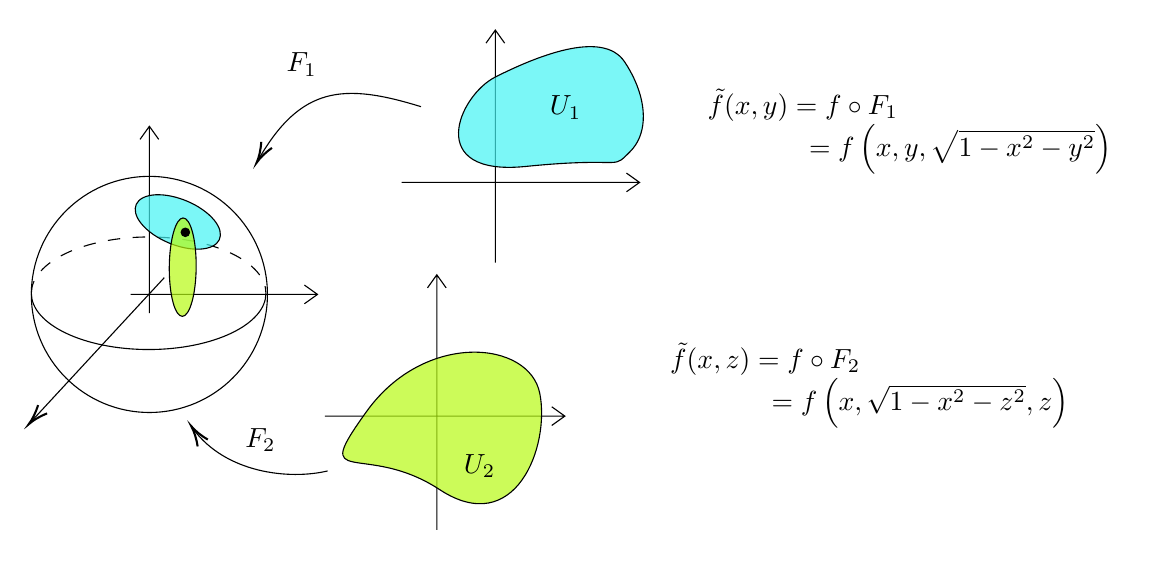
\begin{tikzpicture}[x=0.75pt,y=0.75pt,yscale=-0.9,xscale=0.9]
    %uncomment if require: \path (0,300); %set diagram left start at 0, and has height of 300

    %Shape: Axis 2D [id:dp5905610283034792] 
    \draw  (128,153) -- (228,153)(138,63) -- (138,163) (221,148) -- (228,153) -- (221,158) (133,70) -- (138,63) -- (143,70)  ;
    %Straight Lines [id:da5258527733857374] 
    \draw    (146,144) -- (74.76,221.03) ;
    \draw [shift={(73.4,222.5)}, rotate = 312.76] [color={rgb, 255:red, 0; green, 0; blue, 0 }  ][line width=0.75]    (10.93,-3.29) .. controls (6.95,-1.4) and (3.31,-0.3) .. (0,0) .. controls (3.31,0.3) and (6.95,1.4) .. (10.93,3.29)   ;
    %Shape: Circle [id:dp7596976921705518] 
    \draw   (74.8,153) .. controls (74.8,118.1) and (103.1,89.8) .. (138,89.8) .. controls (172.9,89.8) and (201.2,118.1) .. (201.2,153) .. controls (201.2,187.9) and (172.9,216.2) .. (138,216.2) .. controls (103.1,216.2) and (74.8,187.9) .. (74.8,153) -- cycle ;
    %Shape: Arc [id:dp4458065415749495] 
    \draw  [draw opacity=0] (200.4,152.37) .. controls (200.4,152.37) and (200.4,152.37) .. (200.4,152.37) .. controls (200.4,169.01) and (172.28,182.5) .. (137.6,182.5) .. controls (102.92,182.5) and (74.8,169.01) .. (74.8,152.37) -- (137.6,152.37) -- cycle ; \draw   (200.4,152.37) .. controls (200.4,152.37) and (200.4,152.37) .. (200.4,152.37) .. controls (200.4,169.01) and (172.28,182.5) .. (137.6,182.5) .. controls (102.92,182.5) and (74.8,169.01) .. (74.8,152.37) ;
    %Shape: Arc [id:dp1079879229191647] 
    \draw  [draw opacity=0][dash pattern={on 4.5pt off 4.5pt}] (74.8,152.37) .. controls (74.8,152.37) and (74.8,152.37) .. (74.8,152.37) .. controls (74.8,135.74) and (102.92,122.25) .. (137.6,122.25) .. controls (172.28,122.25) and (200.4,135.74) .. (200.4,152.37) -- (137.6,152.37) -- cycle ; \draw  [dash pattern={on 4.5pt off 4.5pt}] (74.8,152.37) .. controls (74.8,152.37) and (74.8,152.37) .. (74.8,152.37) .. controls (74.8,135.74) and (102.92,122.25) .. (137.6,122.25) .. controls (172.28,122.25) and (200.4,135.74) .. (200.4,152.37) ;
    %Shape: Circle [id:dp8215567727809696] 
    \draw  [fill={rgb, 255:red, 67; green, 243; blue, 243 }  ,fill opacity=0.7 ] (136.48,118.05) .. controls (127.92,110.28) and (128.47,102.27) .. (137.71,100.15) .. controls (146.96,98.03) and (161.39,102.61) .. (169.95,110.38) .. controls (178.51,118.14) and (177.96,126.16) .. (168.71,128.27) .. controls (159.47,130.39) and (145.04,125.81) .. (136.48,118.05) -- cycle ;
    %Shape: Ellipse [id:dp5973540554680155] 
    \draw  [fill={rgb, 255:red, 182; green, 250; blue, 18 }  ,fill opacity=0.7 ] (153.21,114.21) .. controls (156.92,108.46) and (161.1,114.64) .. (162.55,128) .. controls (164.01,141.36) and (162.19,156.86) .. (158.49,162.6) .. controls (154.79,168.35) and (150.6,162.18) .. (149.15,148.81) .. controls (147.69,135.45) and (149.51,119.96) .. (153.21,114.21) -- cycle ;
    %Shape: Circle [id:dp24020151067783413] 
    \draw  [fill={rgb, 255:red, 0; green, 0; blue, 0 }  ,fill opacity=1 ] (155,119.75) .. controls (155,118.51) and (156.01,117.5) .. (157.25,117.5) .. controls (158.49,117.5) and (159.5,118.51) .. (159.5,119.75) .. controls (159.5,120.99) and (158.49,122) .. (157.25,122) .. controls (156.01,122) and (155,120.99) .. (155,119.75) -- cycle ;
    %Shape: Axis 2D [id:dp6541206749950883] 
    \draw  (273,93.05) -- (400.4,93.05)(323.2,11.5) -- (323.2,136) (393.4,88.05) -- (400.4,93.05) -- (393.4,98.05) (318.2,18.5) -- (323.2,11.5) -- (328.2,18.5)  ;
    %Shape: Polygon Curved [id:ds3396588391090478] 
    \draw  [fill={rgb, 255:red, 67; green, 243; blue, 243 }  ,fill opacity=0.7 ] (323.4,36.5) .. controls (343.4,26.5) and (380.4,10.5) .. (392.4,28.5) .. controls (394.54,31.71) and (396.35,34.97) .. (397.81,38.22) .. controls (404.56,53.16) and (404.05,67.85) .. (395.4,76.5) .. controls (386.1,85.8) and (391.98,80.62) .. (356.01,83.08) .. controls (351.25,83.4) and (345.76,83.86) .. (339.4,84.5) .. controls (285,90) and (303.4,46.5) .. (323.4,36.5) -- cycle ;
    %Shape: Axis 2D [id:dp15349087590497468] 
    \draw  (232,218.15) -- (360.4,218.15)(291.87,142.5) -- (291.87,279) (353.4,213.15) -- (360.4,218.15) -- (353.4,223.15) (286.87,149.5) -- (291.87,142.5) -- (296.87,149.5)  ;
    %Shape: Polygon Curved [id:ds9697525934649356] 
    \draw  [fill={rgb, 255:red, 182; green, 250; blue, 18 }  ,fill opacity=0.7 ] (254.4,215.5) .. controls (285.4,172.5) and (341.4,177.5) .. (347,206) .. controls (352.6,234.5) and (333.8,284) .. (293.4,257.5) .. controls (253,231) and (223.4,258.5) .. (254.4,215.5) -- cycle ;
    %Curve Lines [id:da20815011674520578] 
    \draw    (283.4,52.5) .. controls (241.82,39.63) and (218.86,41.46) .. (196.09,81.28) ;
    \draw [shift={(195.4,82.5)}, rotate = 299.29] [color={rgb, 255:red, 0; green, 0; blue, 0 }  ][line width=0.75]    (10.93,-3.29) .. controls (6.95,-1.4) and (3.31,-0.3) .. (0,0) .. controls (3.31,0.3) and (6.95,1.4) .. (10.93,3.29)   ;
    %Curve Lines [id:da056699720507130014] 
    \draw    (233.4,247.5) .. controls (212.82,252.4) and (178.79,248.66) .. (161.44,224.97) ;
    \draw [shift={(160.4,223.5)}, rotate = 55.78] [color={rgb, 255:red, 0; green, 0; blue, 0 }  ][line width=0.75]    (10.93,-3.29) .. controls (6.95,-1.4) and (3.31,-0.3) .. (0,0) .. controls (3.31,0.3) and (6.95,1.4) .. (10.93,3.29)   ;

    % Text Node
    \draw (428,41.4) node [anchor=north west][inner sep=0.75pt]    {$ \begin{array}{l}
                \tilde{f}( x,y) =f\circ F_{1} \\
                \ \ \ \ \ \ \ \ \ \ \ =f\left( x,y,\sqrt{1-x^{2} -y^{2}}\right)
            \end{array}$};
    % Text Node
    \draw (408,177.4) node [anchor=north west][inner sep=0.75pt]    {$ \begin{array}{l}
                \tilde{f}( x,z) =f\circ F_{2} \\
                \ \ \ \ \ \ \ \ \ \ \ =f\left( x,\sqrt{1-x^{2} -z^{2}} ,z\right)
            \end{array}$};
    % Text Node
    \draw (210,22.4) node [anchor=north west][inner sep=0.75pt]    {$F_{1}$};
    % Text Node
    \draw (188,223.4) node [anchor=north west][inner sep=0.75pt]    {$F_{2}$};
    % Text Node
    \draw (351,45.4) node [anchor=north west][inner sep=0.75pt]    {$U_{1}$};
    % Text Node
    \draw (305,237.4) node [anchor=north west][inner sep=0.75pt]    {$U_{2}$};


\end{tikzpicture}

Smoothness is not affected by the coordinate change. Moreover, it's easy to
apply the chain rule to find relation of differentials of f between
different coordinate charts.
\begin{definition}[Differential function]
    $S$ is a regular surface in $\mathbb{R}^3$. A function $f$ is said to
    be differentiable at $p\in S$, if for a local parametrization near $p$
    \[
        x\colon U\subset \mathbb{R}^2\to \mathbb{R}^3,
    \]
    the function $f\circ x\colon \mathbb{R}^2\to \mathbb{R}$ is
    differentiable at $x^{-1}(p)$
\end{definition}
\begin{remark}
    $f\circ x$ is well-defined, since the differentiability is not affected
    by a change of parameter, e.g. if $y\colon V\subset \mathbb{R}^2\to\
        mathbb{R}^3$ is another parametrization near $p$, $f\circ y=f\circ
        x\circ(\underbrace{x^{-1}\circ y}_{\text{change of parameter}})$ is
    differentiable.
\end{remark}
\begin{example}
    Consider $x^2+y^2+(z-1)^2$=1.
    \begin{enumerate}[(1)]
        \item  Consider $\va{X}=(x,y,z)$ be the position vector field in
              $\mathbb{R}^3$. Let $f(x,y,z)=\va{X}\vdot \va{n}$
              where $\va{n}=(0,0,1)$ is the unit normal of $xy$
              plane.
              \begin{center}



                  \tikzset{every picture/.style={line width=0.75pt}} %set default line width to 0.75pt        

                  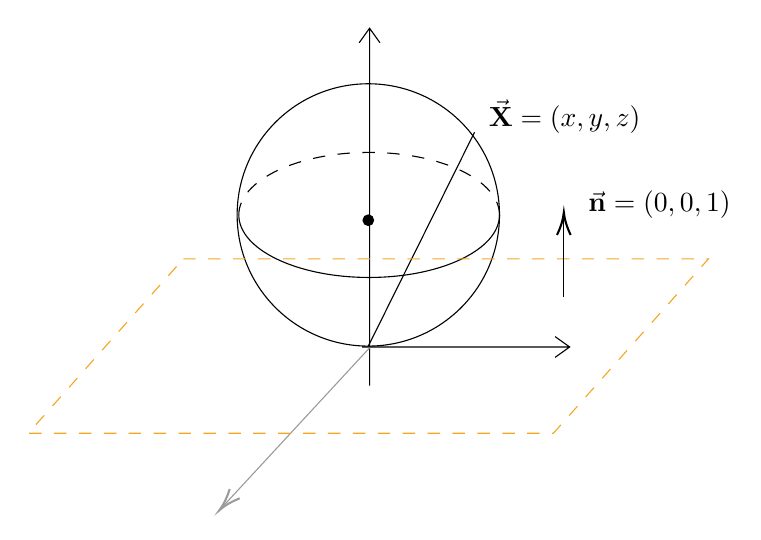
\begin{tikzpicture}[x=0.75pt,y=0.75pt,yscale=-1,xscale=1]
                      %uncomment if require: \path (0,300); %set diagram left start at 0, and has height of 300

                      %Shape: Axis 2D [id:dp5905610283034792] 
                      \draw  (299.2,197) -- (399.2,197)(302.8,43.42) -- (302.8,215.62) (392.2,192) -- (399.2,197) -- (392.2,202) (297.8,50.42) -- (302.8,43.42) -- (307.8,50.42)  ;
                      %Straight Lines [id:da5258527733857374] 
                      \draw [color={rgb, 255:red, 155; green, 155; blue, 155 }  ,draw opacity=1 ]   (303,197.2) -- (260.68,242.96) -- (231.76,274.23) ;
                      \draw [shift={(230.4,275.7)}, rotate = 312.76] [color={rgb, 255:red, 155; green, 155; blue, 155 }  ,draw opacity=1 ][line width=0.75]    (10.93,-3.29) .. controls (6.95,-1.4) and (3.31,-0.3) .. (0,0) .. controls (3.31,0.3) and (6.95,1.4) .. (10.93,3.29)   ;
                      %Shape: Circle [id:dp7596976921705518] 
                      \draw   (239,133.37) .. controls (239,98.47) and (267.3,70.18) .. (302.2,70.18) .. controls (337.1,70.18) and (365.4,98.47) .. (365.4,133.37) .. controls (365.4,168.28) and (337.1,196.57) .. (302.2,196.57) .. controls (267.3,196.57) and (239,168.28) .. (239,133.37) -- cycle ;
                      %Shape: Arc [id:dp4458065415749495] 
                      \draw  [draw opacity=0] (365.4,133.37) .. controls (365.4,150.01) and (337.28,163.5) .. (302.6,163.5) .. controls (267.92,163.5) and (239.8,150.01) .. (239.8,133.37) -- (302.6,133.37) -- cycle ; \draw   (365.4,133.37) .. controls (365.4,150.01) and (337.28,163.5) .. (302.6,163.5) .. controls (267.92,163.5) and (239.8,150.01) .. (239.8,133.37) ;
                      %Shape: Arc [id:dp1079879229191647] 
                      \draw  [draw opacity=0][dash pattern={on 4.5pt off 4.5pt}] (239.8,133.37) .. controls (239.8,116.74) and (267.92,103.25) .. (302.6,103.25) .. controls (337.28,103.25) and (365.4,116.74) .. (365.4,133.37) -- (302.6,133.37) -- cycle ; \draw  [dash pattern={on 4.5pt off 4.5pt}] (239.8,133.37) .. controls (239.8,116.74) and (267.92,103.25) .. (302.6,103.25) .. controls (337.28,103.25) and (365.4,116.74) .. (365.4,133.37) ;
                      %Straight Lines [id:da4102003893399948] 
                      \draw    (353.4,93.5) -- (302.2,196.57) ;
                      %Shape: Circle [id:dp09109443249657256] 
                      \draw  [color={rgb, 255:red, 0; green, 0; blue, 0 }  ,draw opacity=1 ][fill={rgb, 255:red, 0; green, 0; blue, 0 }  ,fill opacity=1 ] (299.65,135.92) .. controls (299.65,134.52) and (300.79,133.37) .. (302.2,133.37) .. controls (303.61,133.37) and (304.75,134.52) .. (304.75,135.92) .. controls (304.75,137.33) and (303.61,138.47) .. (302.2,138.47) .. controls (300.79,138.47) and (299.65,137.33) .. (299.65,135.92) -- cycle ;
                      %Shape: Parallelogram [id:dp22036772290852347] 
                      \draw  [color={rgb, 255:red, 245; green, 166; blue, 35 }  ,draw opacity=1 ][dash pattern={on 4.5pt off 4.5pt}] (213.05,154.57) -- (466.05,154.57) -- (391.35,238.57) -- (138.35,238.57) -- cycle ;
                      %Straight Lines [id:da5141552556306255] 
                      \draw    (396.4,173.1) -- (396.4,134.1) ;
                      \draw [shift={(396.4,132.1)}, rotate = 90] [color={rgb, 255:red, 0; green, 0; blue, 0 }  ][line width=0.75]    (10.93,-3.29) .. controls (6.95,-1.4) and (3.31,-0.3) .. (0,0) .. controls (3.31,0.3) and (6.95,1.4) .. (10.93,3.29)   ;

                      % Text Node
                      \draw (359,76.4) node [anchor=north west][inner sep=0.75pt]    {$\va{X}=( x,y,z)$};
                      % Text Node
                      \draw (407,120.4) node [anchor=north west][inner sep=0.75pt]    {$\va{n} =( 0,0,1)$};


                  \end{tikzpicture}
              \end{center}
              $\Rightarrow f(x,y,z)=z$.
              At point $(x,y,z)\in \mathbb{S^2},\quad z>1$,
              $f(x,y,z)=1+\sqrt{1-x^2-y^2}$, where $x^2+y^2<1$,
              it's a smooth function.
        \item Consider $d^2(x,y,z)=x^2+y^2+z^2=|\va{X}|
                  ^2$, d
              is the distance function on $\mathbb{R}^2$. $d^2|_
                  {\mathbb{S}^2}=2 z= 2f$ in (1), hence it's a smooth
              function.
    \end{enumerate}
\end{example}
\begin{exercise}
    How does the function $f$ look like in other
    coordinate charts?
\end{exercise}
\begin{definition}[Differentiable mapping between two surfaces]
    $S_1,S_2$ are regular surfaces, $\varphi\colon S_1\to
        S_2$ is a mapping that maps $p\in S_1$ to $\varphi(p)
        \in S_2$. We say $\varphi$ is differentiable at $p\in
        S$, if for some parametrization
    \[
        F\colon U_1\to S_1(\ni p),\quad F_2\colon U_2
        \to S_2(\ni \varphi(p))
    \]
    \[
        F_2^{-1}\circ \varphi \circ F_1\colon U_1\to U_2
        \text{ is differentiable at }F_1^{-1}(p).
    \]
    \begin{center}



        \tikzset{every picture/.style={line width=0.75pt}} %set default line width to 0.75pt        

        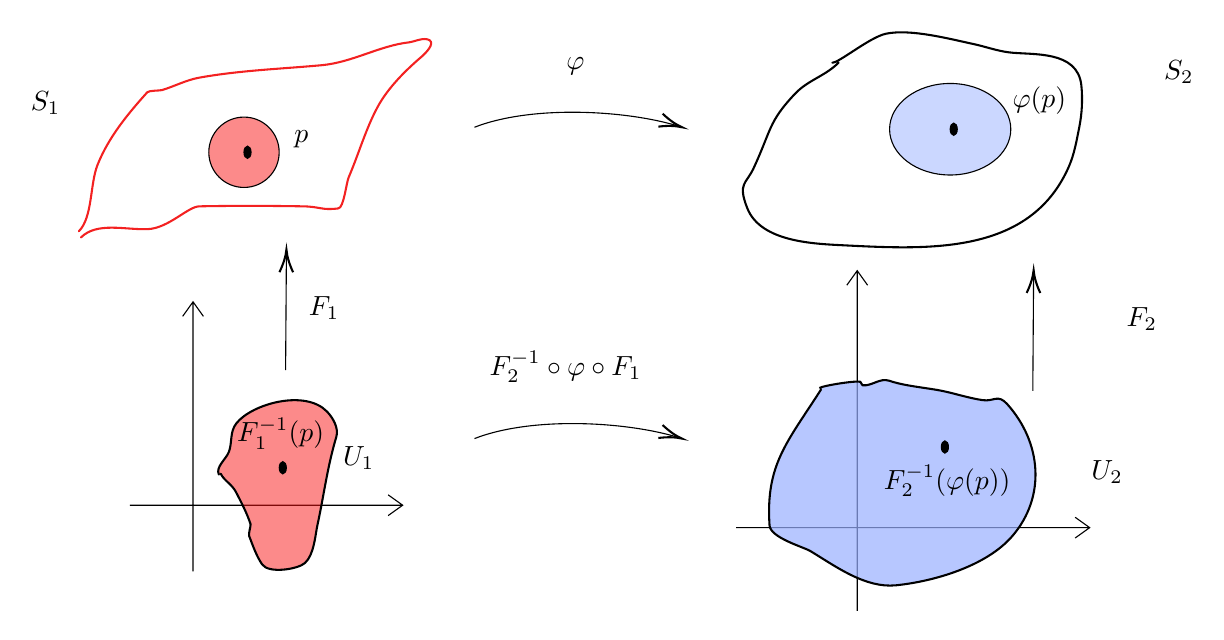
\begin{tikzpicture}[x=0.75pt,y=0.75pt,yscale=-1,xscale=1]
            %uncomment if require: \path (0,300); %set diagram left start at 0, and has height of 300

            %Shape: Axis 2D [id:dp3168627496867378] 
            \draw  (118,241.1) -- (249.4,241.1)(148.4,143.1) -- (148.4,273) (242.4,236.1) -- (249.4,241.1) -- (242.4,246.1) (143.4,150.1) -- (148.4,143.1) -- (153.4,150.1)  ;
            %Curve Lines [id:da7660218913325227] 
            \draw [fill={rgb, 255:red, 250; green, 21; blue, 21 }  ,fill opacity=0.5 ][line width=0.75] [line join = round][line cap = round]   (161.75,225.91) .. controls (163.21,229.11) and (167.16,231.03) .. (169.05,234.68) .. controls (171.65,239.71) and (174.3,244.77) .. (176.1,250.14) .. controls (176.37,250.96) and (175,254.77) .. (175.45,255.94) .. controls (177.24,260.61) and (178.88,265.44) .. (181.67,269.58) .. controls (184.83,274.26) and (198.97,271.92) .. (202.28,268.98) .. controls (206.76,265) and (207.31,255.37) .. (208.3,250.85) .. controls (210.41,241.18) and (211.84,231.78) .. (213.89,222.2) .. controls (214.88,217.6) and (216.01,212.95) .. (217.43,208.21) .. controls (218.67,204.05) and (215.96,199.1) .. (212.94,195.97) .. controls (202.48,185.12) and (176.92,192.17) .. (169.33,201.57) .. controls (166.02,205.68) and (167.34,210.96) .. (165.71,215.31) .. controls (164.35,218.95) and (159.15,222.63) .. (160.84,226.33) ;
            %Shape: Axis 2D [id:dp528543087337018] 
            \draw  (410,251.9) -- (580.4,251.9)(468.4,128.1) -- (468.4,292) (573.4,246.9) -- (580.4,251.9) -- (573.4,256.9) (463.4,135.1) -- (468.4,128.1) -- (473.4,135.1)  ;
            %Curve Lines [id:da3774751912241312] 
            \draw [fill={rgb, 255:red, 152; green, 175; blue, 255 }  ,fill opacity=0.7 ][line width=0.75] [line join = round][line cap = round]   (450.96,185.36) .. controls (434.61,210.92) and (424.22,221.45) .. (426.16,250.82) .. controls (426.55,256.8) and (442.57,261.22) .. (445.85,263.2) .. controls (457.8,270.39) and (472.24,281.19) .. (487.08,279.68) .. controls (505.36,277.82) and (530.67,270.45) .. (543.11,255.99) .. controls (559.48,236.96) and (557.22,210.87) .. (540.68,192.4) .. controls (536.12,187.31) and (534.36,191.29) .. (528.8,190.47) .. controls (521.34,189.36) and (514.15,186.78) .. (506.72,185.52) .. controls (505.84,185.38) and (504.96,185.23) .. (504.08,185.1) .. controls (497.07,184.01) and (489.7,183.15) .. (483.79,181.12) .. controls (479.39,179.6) and (475.39,183.81) .. (470.98,183.32) .. controls (470.32,183.25) and (470.56,181.78) .. (469.91,181.63) .. controls (467.04,180.99) and (451.91,183.57) .. (450.42,184.51) ;
            %Curve Lines [id:da0882085470935694] 
            \draw [color={rgb, 255:red, 243; green, 33; blue, 33 }  ,draw opacity=1 ][line width=0.75] [line join = round][line cap = round]   (93.4,109.1) .. controls (100.05,102.45) and (98.71,86.33) .. (102.4,77.1) .. controls (107.6,64.1) and (116.44,53.16) .. (126.4,42.1) .. controls (127.15,41.27) and (132.47,41.38) .. (133.4,41.1) .. controls (139.46,39.28) and (145.17,36.21) .. (151.4,35.1) .. controls (171.15,31.57) and (190.63,30.9) .. (210.4,29.1) .. controls (225.05,27.77) and (238.4,19.66) .. (252.4,18.1) .. controls (255.06,17.8) and (259.8,15.37) .. (262.4,17.1) .. controls (264.88,18.75) and (260.66,23.16) .. (258.4,25.1) .. controls (250.53,31.85) and (242.37,39.98) .. (237.4,49.1) .. controls (231.72,59.52) and (228.23,71.84) .. (223.4,83.1) .. controls (222.2,85.9) and (221.08,97.77) .. (218.4,98.1) .. controls (210.26,99.12) and (209.8,97.24) .. (201.4,97.1) .. controls (184.74,96.82) and (168.06,96.77) .. (151.4,97.1) .. controls (145.91,97.21) and (136.51,107.77) .. (126.4,108.1) .. controls (115.66,108.45) and (102,104.5) .. (94.4,112.1) ;
            %Shape: Circle [id:dp8242457231671785] 
            \draw  [fill={rgb, 255:red, 250; green, 21; blue, 21 }  ,fill opacity=0.5 ] (156,71.05) .. controls (156,61.69) and (163.59,54.1) .. (172.95,54.1) .. controls (182.31,54.1) and (189.9,61.69) .. (189.9,71.05) .. controls (189.9,80.41) and (182.31,88) .. (172.95,88) .. controls (163.59,88) and (156,80.41) .. (156,71.05) -- cycle ;
            %Flowchart: Connector [id:dp6730161602721307] 
            \draw  [fill={rgb, 255:red, 0; green, 0; blue, 0 }  ,fill opacity=1 ] (172.95,71.05) .. controls (172.95,69.42) and (173.71,68.1) .. (174.65,68.1) .. controls (175.59,68.1) and (176.35,69.42) .. (176.35,71.05) .. controls (176.35,72.68) and (175.59,74) .. (174.65,74) .. controls (173.71,74) and (172.95,72.68) .. (172.95,71.05) -- cycle ;
            %Curve Lines [id:da7923666736724548] 
            \draw [line width=0.75] [line join = round][line cap = round]   (459.4,27.9) .. controls (452.91,34.39) and (444.66,36.25) .. (438.4,42.9) .. controls (425.52,56.58) and (427.19,59.97) .. (418.4,78.9) .. controls (414.97,86.29) and (410.67,85.82) .. (415.4,97.9) .. controls (421.83,114.34) and (447.48,115.15) .. (462.4,115.9) .. controls (503.31,117.95) and (551.77,120.48) .. (570.4,77.9) .. controls (573.02,71.9) and (574.12,65.32) .. (575.4,58.9) .. controls (576.71,52.35) and (577.06,45.54) .. (576.4,38.9) .. controls (574.66,21.51) and (552.34,24.33) .. (541.4,22.9) .. controls (535.63,22.15) and (530.09,20.12) .. (524.4,18.9) .. controls (512.69,16.39) and (494.29,11.52) .. (482.4,13.9) .. controls (474.64,15.45) and (459.72,27.9) .. (456.4,27.9) ;
            %Shape: Ellipse [id:dp613533126996973] 
            \draw  [fill={rgb, 255:red, 152; green, 175; blue, 255 }  ,fill opacity=0.5 ] (484,59.95) .. controls (484,47.77) and (497.07,37.9) .. (513.2,37.9) .. controls (529.33,37.9) and (542.4,47.77) .. (542.4,59.95) .. controls (542.4,72.13) and (529.33,82) .. (513.2,82) .. controls (497.07,82) and (484,72.13) .. (484,59.95) -- cycle ;
            %Flowchart: Connector [id:dp9628105035874008] 
            \draw  [fill={rgb, 255:red, 0; green, 0; blue, 0 }  ,fill opacity=1 ] (513.2,59.95) .. controls (513.2,58.32) and (513.96,57) .. (514.9,57) .. controls (515.84,57) and (516.6,58.32) .. (516.6,59.95) .. controls (516.6,61.58) and (515.84,62.9) .. (514.9,62.9) .. controls (513.96,62.9) and (513.2,61.58) .. (513.2,59.95) -- cycle ;
            %Curve Lines [id:da8375553954915891] 
            \draw    (284,59) .. controls (311.69,48.18) and (357.06,50.76) .. (382.11,58.4) ;
            \draw [shift={(384,59)}, rotate = 198.23] [color={rgb, 255:red, 0; green, 0; blue, 0 }  ][line width=0.75]    (10.93,-3.29) .. controls (6.95,-1.4) and (3.31,-0.3) .. (0,0) .. controls (3.31,0.3) and (6.95,1.4) .. (10.93,3.29)   ;
            %Flowchart: Connector [id:dp6818451228307187] 
            \draw  [fill={rgb, 255:red, 0; green, 0; blue, 0 }  ,fill opacity=1 ] (189.95,223.05) .. controls (189.95,221.42) and (190.71,220.1) .. (191.65,220.1) .. controls (192.59,220.1) and (193.35,221.42) .. (193.35,223.05) .. controls (193.35,224.68) and (192.59,226) .. (191.65,226) .. controls (190.71,226) and (189.95,224.68) .. (189.95,223.05) -- cycle ;
            %Flowchart: Connector [id:dp0890863255330927] 
            \draw  [fill={rgb, 255:red, 0; green, 0; blue, 0 }  ,fill opacity=1 ] (508.95,213.05) .. controls (508.95,211.42) and (509.71,210.1) .. (510.65,210.1) .. controls (511.59,210.1) and (512.35,211.42) .. (512.35,213.05) .. controls (512.35,214.68) and (511.59,216) .. (510.65,216) .. controls (509.71,216) and (508.95,214.68) .. (508.95,213.05) -- cycle ;
            %Straight Lines [id:da6324032020825887] 
            \draw    (553,186) -- (553.39,129.9) ;
            \draw [shift={(553.4,127.9)}, rotate = 90.39] [color={rgb, 255:red, 0; green, 0; blue, 0 }  ][line width=0.75]    (10.93,-3.29) .. controls (6.95,-1.4) and (3.31,-0.3) .. (0,0) .. controls (3.31,0.3) and (6.95,1.4) .. (10.93,3.29)   ;
            %Straight Lines [id:da37379828971916673] 
            \draw    (193,176) -- (193.39,119.9) ;
            \draw [shift={(193.4,117.9)}, rotate = 90.39] [color={rgb, 255:red, 0; green, 0; blue, 0 }  ][line width=0.75]    (10.93,-3.29) .. controls (6.95,-1.4) and (3.31,-0.3) .. (0,0) .. controls (3.31,0.3) and (6.95,1.4) .. (10.93,3.29)   ;
            %Curve Lines [id:da43645247135955967] 
            \draw    (284,209) .. controls (311.69,198.18) and (357.06,200.76) .. (382.11,208.4) ;
            \draw [shift={(384,209)}, rotate = 198.23] [color={rgb, 255:red, 0; green, 0; blue, 0 }  ][line width=0.75]    (10.93,-3.29) .. controls (6.95,-1.4) and (3.31,-0.3) .. (0,0) .. controls (3.31,0.3) and (6.95,1.4) .. (10.93,3.29)   ;

            % Text Node
            \draw (196,59.4) node [anchor=north west][inner sep=0.75pt]    {$p$};
            % Text Node
            \draw (69,40.4) node [anchor=north west][inner sep=0.75pt]    {$S_{1}$};
            % Text Node
            \draw (615,25.4) node [anchor=north west][inner sep=0.75pt]    {$S_{2}$};
            % Text Node
            \draw (542,38.4) node [anchor=north west][inner sep=0.75pt]    {$\varphi ( p)$};
            % Text Node
            \draw (327,24.4) node [anchor=north west][inner sep=0.75pt]    {$\varphi $};
            % Text Node
            \draw (168.43,197.61) node [anchor=north west][inner sep=0.75pt]    {$F_{1}^{-1}( p)$};
            % Text Node
            \draw (480,220.4) node [anchor=north west][inner sep=0.75pt]    {$F_{2}^{-1}( \varphi ( p))$};
            % Text Node
            \draw (597,144.4) node [anchor=north west][inner sep=0.75pt]    {$F_{2}$};
            % Text Node
            \draw (203,139.4) node [anchor=north west][inner sep=0.75pt]    {$F_{1}$};
            % Text Node
            \draw (290,165.4) node [anchor=north west][inner sep=0.75pt]    {$F_{2}^{-1} \circ \varphi \circ F_{1}$};
            % Text Node
            \draw (219.43,211.61) node [anchor=north west][inner sep=0.75pt]    {$U_{1}$};
            % Text Node
            \draw (580,218.4) node [anchor=north west][inner sep=0.75pt]    {$U_{2}$};


        \end{tikzpicture}
    \end{center}
    \underline{Locally}, if $(u,v)$ serves as coordinate of $p$, $F_2^{-1}
        \circ\varphi \circ F_1=(\varphi_1,\varphi_2)$, then $\varphi$ is
    differentiable iff $\varphi^1$ and  $\varphi^2$ are differentiable
    Functions.
\end{definition}
\begin{remark}
    In the future, we won't explicitly write $F_1$ and $F_2$, but simply
    write $\varphi\colon S_1\to S_2$ locally as $\varphi(u,v)=\left(\varphi^1(u,v),\varphi^2(u,v)\right)$.
\end{remark}
\begin{definition}[Diffeomorphism]
    $S_1$ and $S_2$ are regular surfaces. $S_1$ is diffeomorphic to $S_2$
    if $\exists f\colon S_1\to S_2$ such that both $f$ and $f^{-1}$ are
    differentiable.
\end{definition}
\begin{remark}
    Diffeomorphism is the equivalent relation we often use in differential
    geometry. Later, we'll introduce a ``stronger'' equivalent relation after defining the 1st fundamental form.
\end{remark}
\begin{question}
    Can you give an intuitive \underline{example} of ``Diffeomorphism''
    between two surfaces?
\end{question}
\begin{example}
    Identity map/ $\mathbb{R}^2$ with translation action, rotation action/
    $\mathbb{S}^2(1)$ by changing radius.
\end{example}
{\Large\textcolor{red}{\textbf{!}}} {All diffeomorphism of a surface}
is a group. (Lie group) (because the composition (multiplication of the group)
of two diffeomorphism is also a diffeomorphism).
\begin{example}
    ${x^2+y^2+z^2=1}$ is diffeomorphic to ${\left(\frac{x}{a}\right)^2
                +\left(\frac{y}{b}\right)^2+\left(\frac{z}{c}\right)^2=1}(a,b,c\neq 0)$.
\end{example}
\begin{proof}
    Consider $\varphi \colon \mathbb{R}^3\to \mathbb{R}^3$
    \[
        (x,y,z)\mapsto (ax,by,cz).
    \]
    This is a diffeomorphism of $\mathbb{R}^3$.(what is $\varphi|_{\mathbb{S}^2}$?)

    If $p\in \mathbb{S}^2$ lies on the upper semi-sphere, we use
    parametrization
    \[
        F(x,y)=(x,y,\sqrt{1-x^2-y^2})\colon U\subset \mathbb{R}^3\to \mathbb
        {R}^3    .
    \]
    So near $p$
    \[
        \varphi|_{\mathbb{S}^2}=(ax,by,cz)=(u,v,w)\Rightarrow
        \left(\frac{u}{a}\right)^2
        +\left(\frac{v}{b}\right)^2+\left(\frac{w}{c}\right)^2=1
        .\]
    By checking points in other five charts on $\mathbb{S}^2$, we obtain $\varphi\colon \mathbb{S}^2\to \text{ellipsoid}$ is a diffeomorphism. ($\varphi^{-1}$ is self-clear in the above expression.)
\end{proof}
\section{Tangent plane and differential of a map}
$\bullet$ Let $S$ be a regular surface, \(p_0\in S\). In Calculus, we
defined the tangent plane at \(p_0\colon T_{p_0}S\) as follows: if
\(F\colon U\subset \mathbb{R}^2\to \mathbb{R}^3\) is a local parametrization near \(p_0\)
\[
    (u,v)\mapsto \left(x(u,v),y(u,v),z(u,v)\right).
\]
Since \(F\) is regular, \(\Rightarrow \pdv{F}{u}\wedge\pdv
{F}{v}\) is a normal vector of the tangent plane. Hence,
\(T_{p_0}S\) has the equation
\[
    \left(\pdv{F}{u}\wedge\pdv{F}{v}\right)\vdot
    (p-p_0)=0,\quad p\in \mathbb{R}^3  .
\]
However, this definition has some deficiency:
\begin{enumerate}[(1)]
    \item We ``have'' not checked what happened if we change the parameter.

      \textcolor{blue}{(In geometry, whenever you define a concept by using
          some parametrization, you should always check that the concept doesn't
          depend on the choice of your param, so it's a well-defined
          definition.)}
    \item When we write the equation of the tangent plane, we have used
      Euclidean inner product in $\mathbb{R}^3$.

      \textcolor{blue}{(The tangent space should be an intrinsic object, \ie\ it depends on the surface itself only.)}
\end{enumerate}
\begin{definition}[Tangent vector]
    $V$ is called a tangent vector at \(p\in S\) if \(\exists\) a smooth
    curve \(\alpha\colon(-\epsilon,\epsilon)\to S\) with \(\alpha(0)=p\)
    such that \(\alpha'(0)=V\).
    \begin{center}



        \tikzset{every picture/.style={line width=0.75pt}} %set default line width to 0.75pt        

        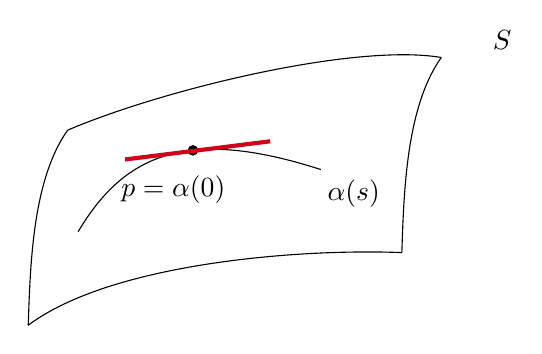
\begin{tikzpicture}[x=0.75pt,y=0.75pt,yscale=-1,xscale=1]
            %uncomment if require: \path (0,300); %set diagram left start at 0, and has height of 300

            %Curve Lines [id:da968109591651267] 
            \draw    (235.4,147.5) .. controls (282.4,127.5) and (374.4,105.5) .. (415.4,112.5) ;
            %Curve Lines [id:da9628832995393517] 
            \draw    (216.4,241.5) .. controls (256.4,211.5) and (347.4,204.5) .. (396.4,206.5) ;
            %Curve Lines [id:da9199503670863729] 
            \draw    (216.4,241.5) .. controls (217.4,212.5) and (218.4,171.5) .. (235.4,147.5) ;
            %Curve Lines [id:da1283058403662014] 
            \draw    (396.4,206.5) .. controls (397.4,177.5) and (398.4,136.5) .. (415.4,112.5) ;
            %Shape: Circle [id:dp20527443514441757] 
            \draw  [fill={rgb, 255:red, 0; green, 0; blue, 0 }  ,fill opacity=1 ] (293.5,157.25) .. controls (293.5,156.01) and (294.51,155) .. (295.75,155) .. controls (296.99,155) and (298,156.01) .. (298,157.25) .. controls (298,158.49) and (296.99,159.5) .. (295.75,159.5) .. controls (294.51,159.5) and (293.5,158.49) .. (293.5,157.25) -- cycle ;
            %Curve Lines [id:da8727495146013418] 
            \draw    (240.4,196.5) .. controls (262.4,159.5) and (292.4,145.5) .. (357.4,166.5) ;
            %Straight Lines [id:da5229930312194522] 
            \draw [color={rgb, 255:red, 208; green, 2; blue, 27 }  ,draw opacity=1 ][line width=1.5]    (263.05,161.63) -- (332.95,152.88) ;

            % Text Node
            \draw (439,98.4) node [anchor=north west][inner sep=0.75pt]    {$S$};
            % Text Node
            \draw (260,168.4) node [anchor=north west][inner sep=0.75pt]    {$p=\alpha ( 0)$};
            % Text Node
            \draw (359.4,169.9) node [anchor=north west][inner sep=0.75pt]    {$\alpha ( s)$};


        \end{tikzpicture}
    \end{center}
\end{definition}
\begin{definition}[Tangent space]
    \(T_p S={\text{all tangent vectors at p}}\).
    (\ie\ Tangent space is the collection of all tangent vectors of
    equivalent classes of curves passing through \(p\).)
\end{definition}
Here, we say two curves \(\alpha_1\colon(-\epsilon,\epsilon)\to S,
\alpha_2\colon(-\epsilon,\epsilon)\to S\) are equivalent at \(p\)
if \(\alpha_1(0)=\alpha_2(0)\) and \(\alpha_1'(0)=\alpha_2'(0)\).
\begin{center}



    \tikzset{every picture/.style={line width=0.75pt}} %set default line width to 0.75pt        

    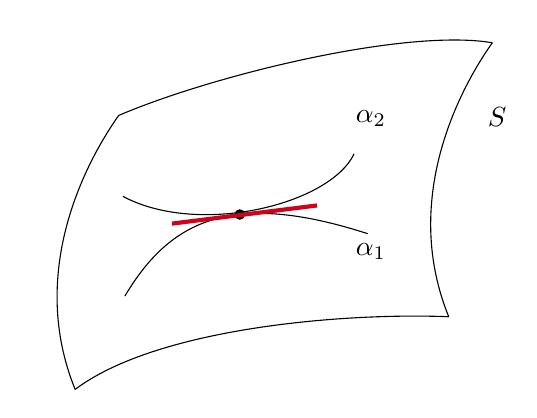
\begin{tikzpicture}[x=0.75pt,y=0.75pt,yscale=-1,xscale=1]
        %uncomment if require: \path (0,300); %set diagram left start at 0, and has height of 300

        %Curve Lines [id:da968109591651267] 
        \draw    (237.4,109.5) .. controls (284.4,89.5) and (376.4,67.5) .. (417.4,74.5) ;
        %Curve Lines [id:da9628832995393517] 
        \draw    (216.4,241.5) .. controls (256.4,211.5) and (347.4,204.5) .. (396.4,206.5) ;
        %Curve Lines [id:da9199503670863729] 
        \draw    (216.4,241.5) .. controls (193.8,186) and (220.4,133.5) .. (237.4,109.5) ;
        %Shape: Circle [id:dp20527443514441757] 
        \draw  [fill={rgb, 255:red, 0; green, 0; blue, 0 }  ,fill opacity=1 ] (293.5,157.25) .. controls (293.5,156.01) and (294.51,155) .. (295.75,155) .. controls (296.99,155) and (298,156.01) .. (298,157.25) .. controls (298,158.49) and (296.99,159.5) .. (295.75,159.5) .. controls (294.51,159.5) and (293.5,158.49) .. (293.5,157.25) -- cycle ;
        %Curve Lines [id:da8727495146013418] 
        \draw    (240.4,196.5) .. controls (262.4,159.5) and (292.4,145.5) .. (357.4,166.5) ;
        %Straight Lines [id:da5229930312194522] 
        \draw [color={rgb, 255:red, 208; green, 2; blue, 27 }  ,draw opacity=1 ][line width=1.5]    (263.05,161.63) -- (332.95,152.88) ;
        %Curve Lines [id:da5488316181309845] 
        \draw    (396.4,206.5) .. controls (373.8,151) and (400.4,98.5) .. (417.4,74.5) ;
        %Curve Lines [id:da7167451379981096] 
        \draw    (239.4,148.5) .. controls (275.8,168) and (339.2,152.5) .. (350.8,128) ;

        % Text Node
        \draw (414,104.4) node [anchor=north west][inner sep=0.75pt]    {$S$};
        % Text Node
        \draw (350.4,169.9) node [anchor=north west][inner sep=0.75pt]    {$\alpha _{1}$};
        % Text Node
        \draw (350.4,105.9) node [anchor=north west][inner sep=0.75pt]    {$\alpha _{2}$};


    \end{tikzpicture}
\end{center}
\begin{remark}
    \hfill
    \begin{enumerate}[(1)]
        \item This definition is sufficient in the following study of the
              course. Later, we will give another definition of tangent space
              by viewing a tangent vector as an operator acting on some equivalent
              class of \(C^\infty\) functions at a point.(\ie\ a tangent vector
              is a ``directional derivative'', which satisfies ``Linearity'' and
              ``Leibniz rule'') This will tell us how to take derivative of a
              function on a surface.
        \item In algebraic geometry course, you'll also see another
              definition of tangent vector (space) of an algebraic variety.
              You should make a comparison with these definitions, This is
              more abstract.
    \end{enumerate}
\end{remark}
\textbf{Claim:} Local expression of tangent vector is independent of the choice of
local param.
\begin{proof}
    Let \(\alpha(s)\colon (-\epsilon,\epsilon)\to S\) be the regular curve
    such that \(\alpha'(0)=V\) for the given tangent vector \(V\) at \(p\).
    Choose a local parametrization near \(p\),
    \begin{align*}
                     & F\colon  U\subset \mathbb{R}^2\to S \\
        (u,v)\mapsto & \left(x(u,v),y(u,v),z(u,v)\right)
        ,\end{align*}
    then \(\alpha(s)=\left(x\left(u(s),v(s)\right),y\left(u(s),v(s)\right),
    z\left(u(s),v(s)\right)\right)\). In fact, if we define
    \[
        \beta(s)=F^{-1}\circ\alpha(s)\colon (-\epsilon,\epsilon)\to U\subset
        \mathbb{R}^2
        ,\]
    then \(\alpha(s)=F\circ \beta (s)\).
    \begin{center}



        \tikzset{every picture/.style={line width=0.75pt}} %set default line width to 0.75pt        

        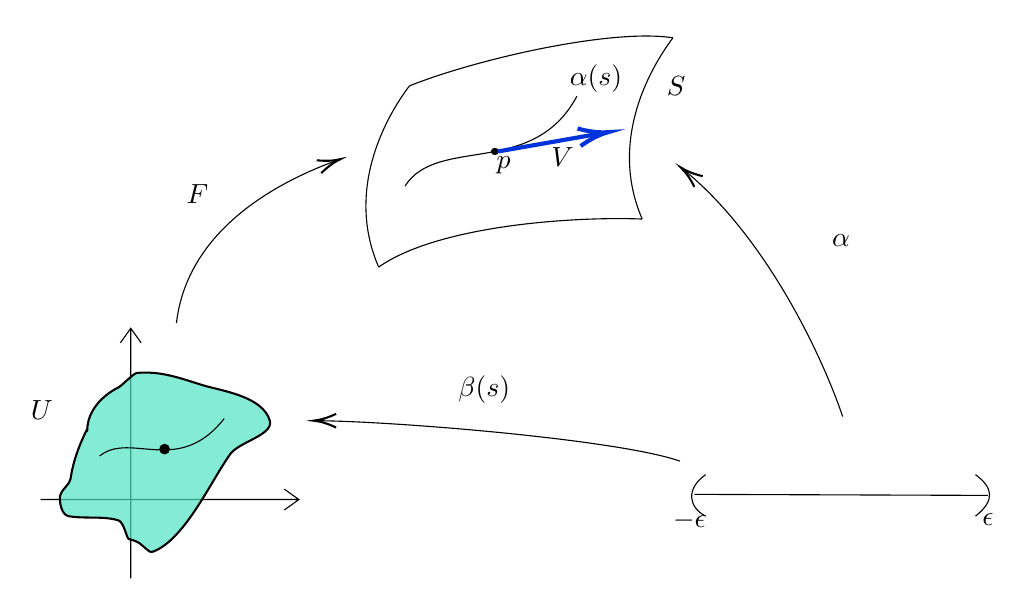
\begin{tikzpicture}[x=0.75pt,y=0.75pt,yscale=-1,xscale=1]
            %uncomment if require: \path (0,300); %set diagram left start at 0, and has height of 300

            %Curve Lines [id:da968109591651267] 
            \draw    (317.65,44.2) .. controls (350.81,30.97) and (415.7,16.42) .. (444.63,21.05) ;
            %Curve Lines [id:da9628832995393517] 
            \draw    (302.84,131.5) .. controls (331.05,111.66) and (395.25,107.03) .. (429.81,108.35) ;
            %Curve Lines [id:da9199503670863729] 
            \draw    (302.84,131.5) .. controls (286.89,94.79) and (305.66,60.07) .. (317.65,44.2) ;
            %Shape: Ellipse [id:dp20527443514441757] 
            \draw  [fill={rgb, 255:red, 0; green, 0; blue, 0 }  ,fill opacity=1 ] (357.22,75.78) .. controls (357.22,74.96) and (357.94,74.29) .. (358.81,74.29) .. controls (359.69,74.29) and (360.4,74.96) .. (360.4,75.78) .. controls (360.4,76.6) and (359.69,77.27) .. (358.81,77.27) .. controls (357.94,77.27) and (357.22,76.6) .. (357.22,75.78) -- cycle ;
            %Curve Lines [id:da8727495146013418] 
            \draw    (315.53,92.48) .. controls (331.05,68.01) and (377.19,88.84) .. (398.35,49.16) ;
            %Curve Lines [id:da5488316181309845] 
            \draw    (429.81,108.35) .. controls (413.87,71.65) and (432.64,36.92) .. (444.63,21.05) ;
            %Straight Lines [id:da7604427159074587] 
            \draw [color={rgb, 255:red, 0; green, 50; blue, 219 }  ,draw opacity=1 ][line width=1.5]    (360.4,75.78) -- (410.44,67.02) ;
            \draw [shift={(413.4,66.5)}, rotate = 170.07] [color={rgb, 255:red, 0; green, 50; blue, 219 }  ,draw opacity=1 ][line width=1.5]    (14.21,-4.28) .. controls (9.04,-1.82) and (4.3,-0.39) .. (0,0) .. controls (4.3,0.39) and (9.04,1.82) .. (14.21,4.28)   ;
            %Straight Lines [id:da8896542176151039] 
            \draw    (455,241) -- (596.4,241.5) ;
            %Curve Lines [id:da5641842523044696] 
            \draw    (460.4,231.5) .. controls (450.4,238.5) and (452.4,247.5) .. (460.4,251.5) ;
            %Curve Lines [id:da015954054171630094] 
            \draw    (590.4,231.5) .. controls (598.4,237.5) and (600.4,243.5) .. (590.4,251.5) ;
            %Curve Lines [id:da04574325182537042] 
            \draw    (526.4,203.5) .. controls (514.52,168.85) and (486.96,114.6) .. (449.54,84.41) ;
            \draw [shift={(448.4,83.5)}, rotate = 38.29] [color={rgb, 255:red, 0; green, 0; blue, 0 }  ][line width=0.75]    (10.93,-3.29) .. controls (6.95,-1.4) and (3.31,-0.3) .. (0,0) .. controls (3.31,0.3) and (6.95,1.4) .. (10.93,3.29)   ;
            %Shape: Axis 2D [id:dp9341218118059429] 
            \draw  (140,243.5) -- (264.4,243.5)(183.4,161) -- (183.4,281.5) (257.4,238.5) -- (264.4,243.5) -- (257.4,248.5) (178.4,168) -- (183.4,161) -- (188.4,168)  ;
            %Curve Lines [id:da5440535940443412] 
            \draw    (205.4,158.5) .. controls (210.32,116.14) and (249.21,92.22) .. (282.87,80.05) ;
            \draw [shift={(284.4,79.5)}, rotate = 160.56] [color={rgb, 255:red, 0; green, 0; blue, 0 }  ][line width=0.75]    (10.93,-3.29) .. controls (6.95,-1.4) and (3.31,-0.3) .. (0,0) .. controls (3.31,0.3) and (6.95,1.4) .. (10.93,3.29)   ;
            %Curve Lines [id:da3824738174976394] 
            \draw [fill={rgb, 255:red, 80; green, 227; blue, 194 }  ,fill opacity=0.7 ][line width=0.75] [line join = round][line cap = round]   (162.4,209.5) .. controls (158.54,217.23) and (155.61,225.06) .. (154.4,233.5) .. controls (153.99,236.38) and (149.97,238.65) .. (149.4,241.5) .. controls (148.84,244.32) and (149.93,250.87) .. (153.4,251.5) .. controls (160.88,252.86) and (170.14,251.32) .. (177.4,253.5) .. controls (180.16,254.33) and (181.45,262.26) .. (182.4,262.5) .. controls (188.34,263.98) and (188.09,265.27) .. (192.4,268.5) .. controls (192.93,268.9) and (193.78,268.75) .. (194.4,268.5) .. controls (209.81,262.34) and (222.3,234.01) .. (231.4,221.5) .. controls (235.62,215.7) and (252.35,212.33) .. (250.4,205.5) .. controls (247.02,193.68) and (226.82,191.06) .. (218.4,188.5) .. controls (207.25,185.11) and (198.45,181.5) .. (186.4,182.5) .. controls (184.71,182.64) and (179.2,188.6) .. (177.4,189.5) .. controls (170.45,192.98) and (162.4,200.22) .. (162.4,210.5) ;
            %Curve Lines [id:da19048774017798897] 
            \draw    (168.4,222.5) .. controls (183.4,210.5) and (206.4,232.5) .. (228.4,204.5) ;
            %Shape: Circle [id:dp7678024484359296] 
            \draw  [fill={rgb, 255:red, 0; green, 0; blue, 0 }  ,fill opacity=1 ] (197.4,219.2) .. controls (197.4,217.93) and (198.43,216.9) .. (199.7,216.9) .. controls (200.97,216.9) and (202,217.93) .. (202,219.2) .. controls (202,220.47) and (200.97,221.5) .. (199.7,221.5) .. controls (198.43,221.5) and (197.4,220.47) .. (197.4,219.2) -- cycle ;
            %Curve Lines [id:da9825567076006667] 
            \draw    (448,225) .. controls (418.84,214.66) and (310.71,205.77) .. (273.07,205.51) ;
            \draw [shift={(271.4,205.5)}, rotate = 360] [color={rgb, 255:red, 0; green, 0; blue, 0 }  ][line width=0.75]    (10.93,-3.29) .. controls (6.95,-1.4) and (3.31,-0.3) .. (0,0) .. controls (3.31,0.3) and (6.95,1.4) .. (10.93,3.29)   ;

            % Text Node
            \draw (440.46,38.25) node [anchor=north west][inner sep=0.75pt]    {$S$};
            % Text Node
            \draw (393.65,32.63) node [anchor=north west][inner sep=0.75pt]    {$\alpha ( s)$};
            % Text Node
            \draw (384.76,72.56) node [anchor=north west][inner sep=0.75pt]    {$V$};
            % Text Node
            \draw (358.46,76.94) node [anchor=north west][inner sep=0.75pt]    {$p$};
            % Text Node
            \draw (443.4,247.9) node [anchor=north west][inner sep=0.75pt]    {$-\epsilon $};
            % Text Node
            \draw (592.4,248.9) node [anchor=north west][inner sep=0.75pt]    {$\epsilon $};
            % Text Node
            \draw (520,114.4) node [anchor=north west][inner sep=0.75pt]    {$\alpha $};
            % Text Node
            \draw (209,90.4) node [anchor=north west][inner sep=0.75pt]    {$F$};
            % Text Node
            \draw (340,182.4) node [anchor=north west][inner sep=0.75pt]    {$\beta ( s)$};
            % Text Node
            \draw (134,194.4) node [anchor=north west][inner sep=0.75pt]    {$U$};


        \end{tikzpicture}
    \end{center}
    \begin{equation}
        V=\alpha'(0)=\left.\pdv{(x,y,z)}{(u,v)}
        \vdot \pdv{(u,v)}{s}\right|_{s=0}\tag{1}
        .\end{equation}
    Now, let \(G\) be another parametrization
    \begin{align*}
                               & G \colon V \to S \\
        (\alpha,\beta) \mapsto &
        \left(x\left(\alpha,\beta\right),y\left(\alpha,\beta\right),
        z\left(\alpha,\beta\right)\right).
    \end{align*}
    Let \(\gamma \colon (-\epsilon,\epsilon)\to V\) be \(\gamma(s)=G^{-1}
    \circ \alpha(s)\colon (-\epsilon,\epsilon)\to V\),
    then \(\alpha(s)=G\circ \gamma(s)\), and
    \begin{equation}
        \alpha'(0)=\left.\pdv{(x,y,z)}{(\alpha,\beta)}\vdot \pdv{(\alpha,\beta)}{s}\right|_{s=0}\tag{2}
        .\end{equation}
    (1) and (2) are essentially the same by the chain rule, \ie\
    \[
        \left.\pdv{(x,y,z)}{(u,v)}
        \vdot \pdv{(u,v)}{s}\right|_{s=0}
        =
        \pdv{(x,y,z)}{(\alpha,\beta)}\vdot
        \underbrace{\pdv{(\alpha,\beta)}{(u,v)}\vdot\pdv{(u,v)}{(\alpha,\beta)}}_{\text{identity matrix}}
        \vdot\left. \pdv{(\alpha,\beta)}{s}
        \right|_{s=0}
    \]
\end{proof}
\begin{proposition}
    Let \(F\colon U\subset \mathbb{R}^2\to S\) be a local parametrization near \(p\) with \(F(q)=p\), then \(dF_q\left(\mathbb{R}^2\right)=T_pS\).
\end{proposition}
\begin{proof}
    \hfill
    \begin{enumerate}[(1)]
        \item \(dF_q\left(\mathbb{R}^2\right)\subset T_p S\)

              \(\forall V\in \mathbb{R}^2\), let \(\beta(t)=q+t V\in \mathbb{R}
              ^2\), then \(\beta'(0)=v\). Let \(\alpha(t)=F\left(\beta(t)\right)
              \) is a \(C^\infty\)- curve passing through \(p\), and
              \[T_p S\ni \alpha'(0)=dF_q\left(\beta'(0)\right)=dF_q(V)\]
        \item \(T_p S\subset dF_q\left(\mathbb{R}^2\right)\)

              \(V\in T_p S\). \(\Rightarrow \exists \alpha(t)\colon (-\epsilon,
              \epsilon)\to S\) such that \(\alpha(0)=p\) and \(\alpha'(0)=V\).
              Let $\beta(t)=F^{-1}\left(\alpha(t)\right)$, then \(\alpha(t)=F
              \left(\beta(t)\right)\). We remark \(\beta(t)\) is a \(C^\infty\)
              -curve in \(\mathbb{R}^2\).(Because we have checked the transition
              function is \(C^\infty\) and \(F^{-1}\) comes from the composition
              of transition function) Thus,
              \[V=\alpha'(0)=dF_q\left(\beta'(0)\right)\in \mathrm{im}\,dF_q\]
    \end{enumerate}
\end{proof}
\begin{remark}
    \hfill
    \begin{enumerate}[(1)]
        \item \(T_p S\) is the full image of linear space under a linear map, thus \(T_pS\) is a linear space of dimension 2.
        \item \(dF_q\) is injective \(\Rightarrow\)\(F_u(q),F_v(q)\) are
              linearly independent, and they are tangent vectors of coordinate
              curve \(F(u,v_0)\) and \(F(u_0,v)\) at \((u_0,v_0)=q\),
              which implies that \(T_pS =\Span\left\{F_u(q),F_v(q)\right\}\).
        \item \(TS=\bigsqcup_{p\in S}T_p S=
              \left\{(p,V)|p\in S,V\in T_pS\right\}\).
              This set can be given a smooth coordinate covering, and is called
              the tangent bundle of \(S\), which is a 4-d smooth manifold. The
              projection
              \begin{align*}
                  \pi\colon TS\to S \\
                  (p,V)\mapsto p
              \end{align*}
              is \(C^\infty\)
    \end{enumerate}
\end{remark}
\subsection*{Tangent vector, tangent space, tangent bundle and tangent vector field}
\begin{enumerate}[(1)]
    \item On \(\mathbb{R}^n\).
    \begin{itemize}
        \item A vector is \(V=(v^1,v^2,\ldots,v^n)\).
        \item A standard basis is \(\{e_1,e_2,\ldots,e_n\}\), where 
        \(e_i=(0,\ldots,\mathop{1}\limits^{i^{th}},\ldots,0)\).\\
        \(\Rightarrow V=\sum_{i=1}^n v^i e_i\).
        \item \(f\) is smooth in \(\mathbb{R}^n\), the directional 
        derivative  along a vector \(v\) at \(p\) is 
        \[
            \left(D_V f\right)(p)=\langle\grad f,V\rangle_p
                =\sum_{i=1}^n v^i\left.\pdv{f}{x^i}\right|_p  
                =\left.\left(\sum_{i=1}^n v^i\pdv{x^i}\right)f\right|_p.
        \]
        Hence, we can identify \(e_i=\pdv{x^i}\) for \(i=1,2,\ldots,n\)
        and shall call \(\pdv{x^i}\) the coordinate vector (field).
        \[
            \Rightarrow V=\sum_{i=1}^n  v^i e_i=\sum_{i=1}^n v^i\pdv
            {x^i}.   
        \]
        \item Note in this way, we actually view a vector \(V\) as a 
        first order linear operator acting on smooth functions, \ie\ 
        for \(p\in \mathbb{R}^n\)
        \[
            V_p \colon  C^\infty\left(\mathbb{R}^n\right)\to \mathbb{R}
        ,\]
        \[ 
            f\mapsto  V(f)(p)=\left(D_V f\right)(p)=\left(v^i\pdv{f}{x^i}
            \right)(p)
        .\]
         Furthermore, this defines
         \[
            V\colon C^\infty\left(\mathbb{R}^n\right)\to 
            C^\infty\left(\mathbb{R}^n\right)   
         \]
         \[
            f\mapsto V(f)   
         .\]
        The operator \(V\) satisfies
        \[
            \begin{cases}
                (V+k W)f=V(f)+kW(f)&\text{(Linearity)}\\
                V(fg)=V(f)g +f V(g)&\text{(Leibniz rule)}
            \end{cases}    
        \]
    \end{itemize}
    \item \(S\) is a regular surface in \(\mathbb{R}^3\), \(p\in S\)
    \begin{itemize}
        \item \(C^\infty(S)={\text{all smooth functions on }S}\).
        \item We have defined \(V\in T_p S\), if \(\exists\) a smooth
        curve \(\alpha\colon (-\epsilon,\epsilon)\to S\) such that
        \(\alpha(t)=p\), \(\alpha'(0)=V\).
        \item To compute \(V\), we choose a local parametrization
        \begin{align*}
            F\colon U(\subset \mathbb{R}^2) &\longrightarrow S\subset \mathbb{R}^3\\
            (y^1,y^2) &\longmapsto (x^1,x^2,x^3)
        .\end{align*}
        \(\Rightarrow \alpha(s)=F\left(y^1(s),y^2(s)\right)\) (This is to 
        say we consider 
        \(\alpha\colon(-\epsilon,\epsilon)\to U
        \mathop{\longrightarrow }\limits^{F} S\)).
        \[
            \Rightarrow V=\alpha'(0)=\left.
            \left(
            \sum_{i=1}^2\pdv{x^1}{y^i}\dv{y^i}{s},
            \sum_{i=1}^2\pdv{x^2}{y^i}\dv{y^i}{s},
            \sum_{i=1}^2\pdv{x^3}{y^i}\dv{y^i}{s}
            \right)
            \right|_{p(s=0)}.
        \]
        Notice \(V\) is a vector in \(\mathbb{R}^3\), by using notation
        in (1)
        \[
            V_p=\sum_{\alpha=1}^3\left(\sum_{i=1}^2\pdv{x^\alpha}{y^i}
            \dv{y^i}{s}\right)\left. \pdv{x^\alpha}  \right|_p.
        \]
        Clearly, the linearity and Leibniz rule hold for the 
        \[
            V_p\colon C^\infty(S)\to \mathbb{R}    
        \]
        \[
            f\mapsto V_p(f)=\left(\left(\sum_{\alpha=1}^3 \sum_{i=1}
            ^2 \pdv{x^\alpha}{y^i}\dv{y^i}{s}\pdv{x^\alpha}\right)f\right)
            (p)   \tag{a} 
        .\]
        Note that during the lecture, we have shown
        \[
            T_pS=dF_{F^{-1}(p)}\left(\mathbb{R}^2\right)=\Span
            \left\{F_{y^1},F_{y^2}\right\}    .
        \]
        Moreover, 
        \[
            F_{y^i}=\sum_{\alpha=1}^3\pdv{x^\alpha}{y^i}\pdv
            {x^\alpha},
        \] 
        by using the notation in (1), and we can write
        \[
            F_{y^i}=\pdv{F}{y^i}=dF_{F^{-1}(p)}\left(\pdv{y^i}\right),
            ~i=1,2.
        \]
        \[
            \Rightarrow T_p S=\Span\left\{
                dF_{F^{-1}(p)}\left(\pdv{y^1}\right),
                dF_{F^{-1}(p)}\left(\pdv{y^2}\right)
            \right\}  ,
        \]
        since \(dF_{F^{-1}(p)}\colon \mathbb{R}^2\to T_p S\) is a linear
        isomorphism. By abusing notation here (actually not)
        \[
            T_p S=\Span \left\{\pdv{y^1},\pdv{y^2}\right\}    
        ,\]
        and 
        \[
            V_p (f)=\left(\sum_{i=1}^2\dv{y^i}{s}\pdv{y^i}\right)(f)(p)    
        .\]
        Hence,
        \[
            T_p S=\{\text{all tangent vectors }v\text{ at }p\}.    
        \]
    \end{itemize}
    \begin{remark}
        If \(M\) is a smooth manifold of dimension \(n\). By definition,
        \(M\) is a topological manifold (\ie\ Hausdorff + second countable 
        + locally Euclidean) that admits a smooth structure, which means 
        that \(\exists\) a covering \(\left\{(U_\alpha,\varphi_\alpha)
        \right\}_{\alpha\in \Lambda}\) of \(M\) such that
        \begin{itemize}
            \item \(\varphi_\alpha\colon U_\alpha\to \varphi
            \left(U_\alpha\right)\subset \mathbb{R}^n\) is a 
            homeomorphism.
            \item \(\varphi_\beta\circ \varphi_\alpha^{-1}\colon
            \varphi_\alpha\left(U_\alpha\cap U_\beta\right)
            \to \varphi_\beta\left(U_\alpha\cap U_\beta\right)
            \)
            is \(C^\infty\), \(\forall\alpha,\beta\) such that 
            \(U_\alpha\cap U_\beta\neq \emptyset\).
        \end{itemize}
        \begin{center}
            


\tikzset{every picture/.style={line width=0.75pt}} %set default line width to 0.75pt        

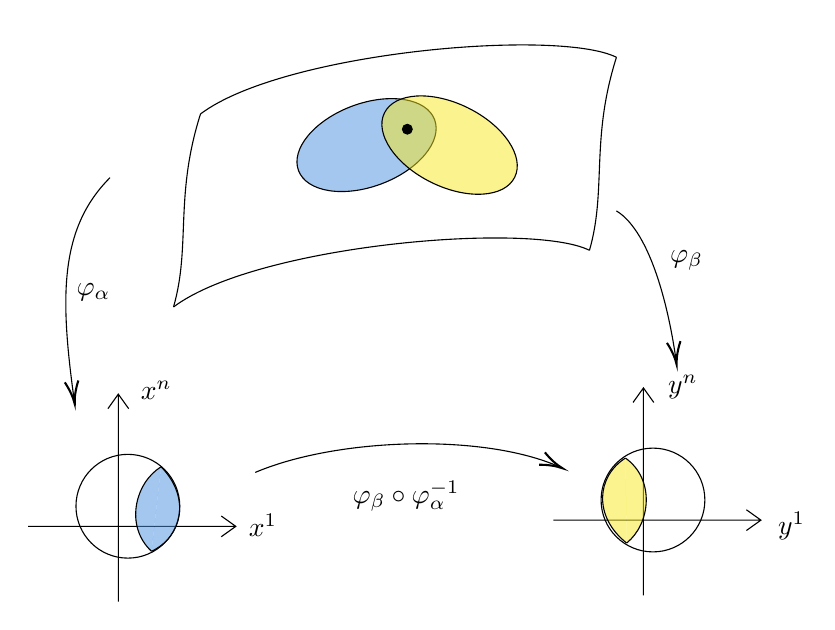
\begin{tikzpicture}[x=0.75pt,y=0.75pt,yscale=-1,xscale=1]
%uncomment if require: \path (0,300); %set diagram left start at 0, and has height of 300

%Curve Lines [id:da41714902560158285] 
\draw    (170,42) .. controls (210,12) and (342.4,0.7) .. (370.4,14.7) ;
%Curve Lines [id:da6592280103805965] 
\draw    (157,135) .. controls (197,105) and (329.4,93.7) .. (357.4,107.7) ;
%Curve Lines [id:da03942270080974852] 
\draw    (157,135) .. controls (165.4,105.7) and (157.4,81.7) .. (170,42) ;
%Curve Lines [id:da4108174147194943] 
\draw    (357.4,107.7) .. controls (365.8,78.4) and (357.8,54.4) .. (370.4,14.7) ;
%Shape: Ellipse [id:dp09147366462581186] 
\draw  [fill={rgb, 255:red, 74; green, 144; blue, 226 }  ,fill opacity=0.5 ] (217.21,69.25) .. controls (213.35,58.9) and (224.89,45.03) .. (243,38.26) .. controls (261.11,31.5) and (278.92,34.41) .. (282.79,44.75) .. controls (286.65,55.1) and (275.11,68.97) .. (257,75.74) .. controls (238.89,82.5) and (221.08,79.59) .. (217.21,69.25) -- cycle ;
%Shape: Ellipse [id:dp0011277621777061597] 
\draw  [fill={rgb, 255:red, 248; green, 231; blue, 28 }  ,fill opacity=0.5 ] (258.61,41.52) .. controls (263.49,31.61) and (281.51,30.51) .. (298.85,39.06) .. controls (316.18,47.61) and (326.28,62.57) .. (321.39,72.48) .. controls (316.51,82.39) and (298.49,83.49) .. (281.15,74.94) .. controls (263.82,66.39) and (253.72,51.43) .. (258.61,41.52) -- cycle ;
%Shape: Circle [id:dp9698509963450805] 
\draw  [fill={rgb, 255:red, 0; green, 0; blue, 0 }  ,fill opacity=1 ] (267.3,49.35) .. controls (267.3,48.05) and (268.35,47) .. (269.65,47) .. controls (270.95,47) and (272,48.05) .. (272,49.35) .. controls (272,50.65) and (270.95,51.7) .. (269.65,51.7) .. controls (268.35,51.7) and (267.3,50.65) .. (267.3,49.35) -- cycle ;
%Shape: Axis 2D [id:dp6551476919278265] 
\draw  (87,240.7) -- (187,240.7)(130.4,177) -- (130.4,277) (180,235.7) -- (187,240.7) -- (180,245.7) (125.4,184) -- (130.4,177) -- (135.4,184)  ;
%Shape: Circle [id:dp177276713898743] 
\draw   (110,231) .. controls (110,217.19) and (121.19,206) .. (135,206) .. controls (148.81,206) and (160,217.19) .. (160,231) .. controls (160,244.81) and (148.81,256) .. (135,256) .. controls (121.19,256) and (110,244.81) .. (110,231) -- cycle ;
%Curve Lines [id:da6569656679367748] 
\draw [fill={rgb, 255:red, 74; green, 144; blue, 226 }  ,fill opacity=0.5 ]   (151,212) .. controls (138.4,219.7) and (133.4,240.7) .. (146.4,252.7) ;
%Curve Lines [id:da7123507841915766] 
\draw [fill={rgb, 255:red, 74; green, 144; blue, 226 }  ,fill opacity=0.5 ]   (151,212) .. controls (165.4,226.7) and (161.4,245.7) .. (146.4,252.7) ;

%Shape: Axis 2D [id:dp8381858872649515] 
\draw  (340,237.7) -- (440,237.7)(383.4,174) -- (383.4,274) (433,232.7) -- (440,237.7) -- (433,242.7) (378.4,181) -- (383.4,174) -- (388.4,181)  ;
%Shape: Circle [id:dp1821947594932496] 
\draw   (363,228) .. controls (363,214.19) and (374.19,203) .. (388,203) .. controls (401.81,203) and (413,214.19) .. (413,228) .. controls (413,241.81) and (401.81,253) .. (388,253) .. controls (374.19,253) and (363,241.81) .. (363,228) -- cycle ;
%Curve Lines [id:da681192978192037] 
\draw [fill={rgb, 255:red, 248; green, 231; blue, 28 }  ,fill opacity=0.5 ]   (375.31,248.74) .. controls (386.84,239.52) and (389.15,218.05) .. (374.74,207.79) ;
%Curve Lines [id:da017656322535560598] 
\draw [fill={rgb, 255:red, 248; green, 231; blue, 28 }  ,fill opacity=0.5 ]   (375.31,248.74) .. controls (359.17,235.98) and (360.74,216.63) .. (374.74,207.79) ;

%Curve Lines [id:da09702567177122501] 
\draw    (370.4,88.7) .. controls (387.36,99.13) and (395.96,137.7) .. (399.16,160.94) ;
\draw [shift={(399.4,162.7)}, rotate = 262.57] [color={rgb, 255:red, 0; green, 0; blue, 0 }  ][line width=0.75]    (10.93,-3.29) .. controls (6.95,-1.4) and (3.31,-0.3) .. (0,0) .. controls (3.31,0.3) and (6.95,1.4) .. (10.93,3.29)   ;
%Curve Lines [id:da6721304677149988] 
\draw    (126.4,72.7) .. controls (101.65,97.45) and (102.38,131.02) .. (109.19,180.2) ;
\draw [shift={(109.4,181.7)}, rotate = 262.03] [color={rgb, 255:red, 0; green, 0; blue, 0 }  ][line width=0.75]    (10.93,-3.29) .. controls (6.95,-1.4) and (3.31,-0.3) .. (0,0) .. controls (3.31,0.3) and (6.95,1.4) .. (10.93,3.29)   ;
%Curve Lines [id:da9747233759845033] 
\draw    (196.4,214.7) .. controls (235.8,197.95) and (306.25,195.76) .. (342.76,211.95) ;
\draw [shift={(344.4,212.7)}, rotate = 205.28] [color={rgb, 255:red, 0; green, 0; blue, 0 }  ][line width=0.75]    (10.93,-3.29) .. controls (6.95,-1.4) and (3.31,-0.3) .. (0,0) .. controls (3.31,0.3) and (6.95,1.4) .. (10.93,3.29)   ;

% Text Node
\draw (395,106.4) node [anchor=north west][inner sep=0.75pt]    {$\varphi _{\beta }$};
% Text Node
\draw (109,122.4) node [anchor=north west][inner sep=0.75pt]    {$\varphi _{\alpha }$};
% Text Node
\draw (242,217.4) node [anchor=north west][inner sep=0.75pt]    {$\varphi _{\beta } \circ \varphi _{\alpha }^{-1}$};
% Text Node
\draw (192,233.4) node [anchor=north west][inner sep=0.75pt]    {$x^{1}$};
% Text Node
\draw (140,169.4) node [anchor=north west][inner sep=0.75pt]    {$x^{n}$};
% Text Node
\draw (447,232.4) node [anchor=north west][inner sep=0.75pt]    {$y^{1}$};
% Text Node
\draw (394,166.4) node [anchor=north west][inner sep=0.75pt]    {$y^{n}$};


\end{tikzpicture}
        \end{center}
        Note that \(\varphi_\alpha\colon U_\alpha \to \varphi_\alpha
        \left(U_\alpha\right)\) actually endow a coordinate on the chart
         \(U_\alpha\), \ie\ \(p\in U_\alpha\), \(\varphi_\alpha(p)
         =\left(x^1(p),x^2(p),\ldots,x^n(p)\right).
         \)
         Hence, \(p\in M\), choose \(U_\alpha\) as its coordinate chart
         \[
            \Rightarrow T_p M=\Span\left\{\pdv{x^1},\ldots,\pdv{x^n}
            \right\}.
         \]
         Note that if at \(p\), there are two coordinate charts
         \[
             \left\lbrace U,\left(x^1,\ldots,x^n\right)\right\rbrace
             \text{ and } 
             \left\lbrace V,\left(y^1,\ldots,y^n\right)\right\rbrace,
         \]
         and a vector \(V\in T_p S\) is expressed as 
         \[
            V=\sum_{i=1}^n V^i\pdv{x^i}=\sum_{\alpha=1}^n 
            \widetilde{V}^\alpha \pdv{y^\alpha}   
         ,\]
         then 
         \[
                \widetilde{V}^\alpha=V^i\pdv{y^\alpha}{x^i}
            \]
    \end{remark}
    \item Tangent (vector) bundle
    
    In (2), we have seen that the tangent space \(T_p S\) of a regular 
    surface does not depend on how we ``put'' \(S\) inside 
    \(\mathbb{R}^3\), and that \(T_p S=\Span\left\{\pdv{y^1},\pdv{y^2}
    \right\}\) for \(\left(y^1,y^2\right)\) a local coordinate in a 
    neighborhood of \(p\). This discussion holds for any smooth manifold.

    In the following, let's just give the general discussion.
    \begin{itemize}
        \item Let \(M\) be a smooth manifold, \(\forall p\in M\), 
        \(T_p M\) is the tangent space at \(p\). Define
        \[
            TM=\bigsqcup_{p\in M}T_p M=\left\{(p,V)| p\in M, V\in 
            T_p M\right\}   
        ,\]
        then there is a projection map 
        \[
            \pi\colon TM\to M
            \]
        \[
            (p,V)\mapsto p.      
            \]
        We shall show that the total space of \(TM\to M\) is a \(2n\)-dim
        smooth manifold such that \(\pi\colon TM \to M\) is a smooth map. 
        To achieve this goal, we need to define a smooth structure on the 
        total space \(TM\).
        \item \(M\) is a smooth manifold, by definition, \(\exists\) a
        countable covering \(\left\{\left(U\alpha,\varphi_\alpha\right)
        \right\}_{\alpha\in \Lambda}\) such that
        \begin{itemize}
            \item \(\varphi_\alpha\colon U_\alpha\to \varphi
            \left(U_\alpha\right)\subset \mathbb{R}^n\) is a 
            homeomorphism,
            \[
                \varphi_\alpha(p)=\left(x^1_\alpha(p),
                x^2_\alpha(p),\ldots,x^n_\alpha(p)\right).
            \]
            \item \(\varphi_\beta\circ \varphi_\alpha^{-1}\colon
            \varphi_\alpha\left(U_\alpha\cap U_\beta\right)
            \to \varphi_\beta\left(U_\alpha\cap U_\beta\right)
            \) is smooth, \(\forall\alpha,\beta\) such that 
            \(U_\alpha\cap U_\beta\neq \emptyset\).
        \end{itemize}
        \item For each \(U_\alpha\), \(\pi^{-1}\left(U_\alpha\right)\)
        contains all pairs \((p,V),p\in U_\alpha,V\in T_p M\). We define
        local trivialization (an local coordinate chart near \((p,V)\) 
        by letting 
        \[
            \widetilde{\varphi}_\alpha\colon 
            \pi^{-1}\left(U_\alpha\right)\to U_\alpha\times 
            \mathbb{R}^n
        \]
        \[
            (p,V)\mapsto \left(\varphi_\alpha(p),V^1,V^2,\ldots,
            V^n\right).    
        \]
        Note \(\widetilde{\varphi}_\alpha(p)=\left(x^1_\alpha(p)
        ,x^2_\alpha(p),\ldots,x^n_\alpha(p)\right)\), 
        \(V=\sum_{i=1}^n V^i(p)\pdv{x^i}\), then
        \[\widetilde{\varphi}_\alpha^{-1}\left(x^1_\alpha
        ,\ldots,x^n_\alpha;V^1,\ldots,V^n\right)=
        \left(p,\sum V^i \pdv{x^i}\right)
        ,\]
        \ie\ \(\widetilde{\varphi}_\alpha\) is bijective and
        \(\widetilde{\varphi}_\alpha\left(\pi^{-1}\left(
            U_\alpha
        \right)\right)\) is an open set.
        Then \(\left\{\widetilde{\varphi}_\alpha^{-1}\left(
            U_\alpha\times \mathbb{R}^n
        \right)\right\}_{\alpha\in \Lambda}\)
        is a countable covering of \(TM\).
        Moreover, this defines a topology on \(TM\), such that
        \[
            \widetilde{\varphi}_\alpha\colon \pi^{-1} 
            \left(U_\alpha\right) \to U_\alpha \times{R}^n  
        \]
        is a homeomorphism.
        Next, if \(\pi^{-1}\left(U_\alpha \right)\cap
        \pi^{-1}\left(U_\beta\right)\neq \emptyset\left(
            \Leftrightarrow U_\alpha\cap U_\beta\neq \emptyset
        \right)\), let \(p\in U_\alpha\cap U_\beta\)
        and 
        \[
            \widetilde{\varphi}_\alpha(p,V)
            = \left(x^1_\alpha(p),
            \cdots,x^n_\alpha(p);
            V^1_\alpha,\ldots,V^n_\alpha
            \right)
        \]
        \[
            \widetilde{\varphi}_\beta(p,V)
            = \left(x^1_\beta(p),
            \cdots,x^n_\beta(p);
            V^1_\beta,\ldots,V^n_\beta
            \right) 
        \]
        \begin{align*}
            \Rightarrow
            \widetilde{\varphi}_\beta\circ 
            \widetilde{\varphi}_\alpha^{-1}
            \left(
                x^1_\alpha(p),
            \cdots,x^n_\alpha(p);
            V^1_\alpha,\ldots,V^n_\alpha
            \right)
            \\=
            \left(x^1_\beta(p),
            \cdots,x^n_\beta(p);
            V^1_\beta,\ldots,V^n_\beta
            \right), 
        \end{align*}
            where
            \[
                V_p=\sum_{i=1}^n V^i_\alpha \pdv{x_\alpha^i}
                =\sum_{j=1}^n V^j_\beta\pdv{x_\beta^j}  
            \]
            \[
                V^j_\beta=\sum_{i=1}^n V^i_\alpha 
                \pdv{y^j_\beta}{x^i_\alpha}    
            ,\]
        \ie\ 
        \begin{align*}
            &\widetilde{\varphi}_\beta\circ 
            \widetilde{\varphi}_\alpha^{-1}
            \left(
                x^1_\alpha(p),
            \cdots,x^n_\alpha(p);
            V^1_\alpha,\ldots,V^n_\alpha
            \right)
            \\&=
            \left(
                \varphi_\beta\circ \varphi_\alpha^{-1}
                \left(x^1_\alpha,\ldots,x^n_\alpha\right);
                \sum_{i=1}^n V^i_\alpha 
                \pdv{y^1_\beta}{x^i_\alpha},
                \cdots,
                \sum_{i=1}^n V^i_\alpha 
                \pdv{y^n_\beta}{x^i_\alpha}
            \right)
        .\end{align*}
        Hence, \(\widetilde{\varphi}_\beta\circ 
        \widetilde{\varphi}_\alpha^{-1}\) is smooth since 
        \(\varphi_\beta\circ \varphi_\alpha^{-1}\)
        is smooth, and the transition function on the vector part 
        is just linear.
        \item The Hausdorff property of \(TM\) is also clear from 
        the Hausdorff property of \(M\).
        \item With the smooth structure defined above, Clearly
        \(\pi\colon TM\to M\) is a smooth map since \(\pi\) is
        just a projection (when expressed in coordinate).
    \end{itemize}
\end{enumerate}
    \textbf{Tangent vector field}
        
\begin{definition}
            A smooth vector field \(V\) is a \(C^\infty\)-map
            \[
                V\colon M\to TM    
            \]
            such that \(\pi\circ V=\mathrm{id}_M\). In a coordinate
            chart \(\left(U_\alpha,\left(x^1_\alpha,\ldots
            x^n_\alpha
            \right)\right)\), \[
              V=\sum_{i=1}^n V^i_\alpha(x)\pdv{x^i_\alpha} 
            \]
\end{definition}
\begin{remark}
            \hfill
        \begin{enumerate}[(1)]
                \item A smooth vector field is also called a smooth
                section of the tangent (vector) bundle.
                \item Since the tangent vector is linear and satisfies
                the Leibniz rule, so is the vector field. Hence,
                \[
                    V\colon C^\infty(M)\to C^\infty(M)    
                \]
                \[
                    f\mapsto V(f)    
                \]
                is characterized by 
                \(V(fg)=V(f)g+fV(g)\).
        \end{enumerate}
\end{remark}
\begin{exercise}
    \hfill
    \begin{enumerate}[(1)]
        \item \(\mathbb{S}^1\): unit circle. 
        \(T\mathbb{S}^1\simeq \mathbb{S}^1 \times \mathbb{R}\) 
        is a diffeomorphism.
        
        Intuitive observation of this diffeomorphism: we can
        choose local charts on \(\mathbb{S}^1\) by 
        \[\theta\in (0,2\pi)=U, ~\varphi \in 
        (\frac{\pi}{2},\frac{3\pi}{2})=V\]
        \ie\ \(\varphi=\theta+\frac{\pi}{2}\), which is simply
        a rotation. 
        \[\left.T\mathbb{S}^1\right|_U=\left\{
            \left(\theta,a(\theta)\pdv{\theta}\right)
        \right\}\]
        \[
            \left.T\mathbb{S}^1\right|_V=\left\{
            \left(\varphi,a(\varphi)\pdv{\varphi}\right)
            \right\}   
        .\]
        In this case, 
        the transition function is just linear by rotation.
        Hence, \(\left.T\mathbb{S}^1\right|_U\) and 
        \(\left.T\mathbb{S}^1\right|_V\) can be glued by shifting 
        \(\frac{\pi}{2}\).
        \item \(\mathbb{S}^2\) unit sphere.
        However, \(T\mathbb{S}^2\ncong \mathbb{S}^2\times 
        \mathbb{R}^2\).
        To see this, we take stereographical parametrization.
        (Since there are only two coordinate charts)
        \begin{align*}
            p_N\colon &\mathbb{S}^2-\{N\}\to \mathbb{R}^2\\
            (x,y,z)&\mapsto \left(\frac{x}{1-z},\frac{y}{1-z}\right)    
        \end{align*}
        \begin{align*}
            p_S\colon &\mathbb{S}^2-\{S\}\to \mathbb{R}^2\\
            (x,y,z)&\mapsto \left(\frac{y}{1+z},\frac{x}{1+z}\right)    
        .\end{align*}
        The transition function is given by 
        \[
          p_S\circ p_N^{-1}(x,y)=\left(\frac{y}{x^2+y^2},
          \frac{x}{x^2+y^2}\right)=(u,v)  
        \]
        \[
            \Rightarrow
            \begin{cases}
                \pdv{x}=-2uv\pdv{u}+\left(v^2-u^2\right)\pdv{v}\\
                \pdv y= \left(u^2-v^2\right)\pdv{u}
                -2uv\pdv{v}
            \end{cases}    
        .\]  
        Note \((x,y)=(0,0)\) is just the north pole and 
        \((u,v)=(0,0)\) is just the south pole. 
        At these two points, the coordinate vector fields 
        are zero vectors, e.g. \(\pdv{x},\pdv{y}\) are zero
        vectors at the south pole.
        This means that we can not extend the tangent 
        plane in the trivialization 
        \(p_N^{-1}\left(\mathbb{R}^2\right)\)
        passing through the south pole, hence we can not
        have a global trivialization of \(T\mathbb{S}^2\).
         \(T\mathbb{S}^2\ncong \mathbb{S}^2\times 
         \mathbb{R}^2\)
    \end{enumerate}         
\end{exercise}
Next, we would like to mention a more abstract way to think 
about the tangent space.
\begin{itemize}
    \item \(M\) is a smooth manifold, \(p\in M\)
    \item \(C_p^\infty(M)\)=\{all \(C^\infty\) functions
    on \(M\) vanishing at \(p\)\}.\\
    \(C_p^\infty(M)^2\)=\{all finite sums 
    \(\sum f_i g_i \) with \(f_i,g_i\in C_p^\infty(M)\)\}
    \[
        \Rightarrow C^\infty(M)=
        \left\{\text{constant functions}\right\}\oplus 
        C^\infty_p(M)=\mathbb{R}\oplus C^\infty_p(M).     
    \]
    \item Let \(V\) be an tangent vector at \(p\), 
    \(V\colon C^\infty(M)\to \mathbb{R}\) and \(V|_{\mathbb{R}}=0\).
    Moreover, it's easy to see by the Leibniz rule that 
    \(V|_{C_p^\infty(M)^2}=0\)
    \[
          \Rightarrow V\colon C_p^\infty(M)/C_p^\infty(M)^2
          \to \mathbb{R}
    \]
    is a linear map, \ie\ \(V\in 
    \left(C_p^\infty(M)/C_p^\infty(M)^2\right)^*\)

    \(\Rightarrow T_p M\simeq 
    \left(C_p^\infty(M)/C_p^\infty(M)^2\right)^*\)
    is an isomorphism. Hence, we can define tangent space
    \(T_p M\) as 
    \(\left(C_p^\infty(M)/C_p^\infty(M)^2\right)^*\)

    This definition tells that a tangent vector is a linear map 
    on \(C^\infty(M)\) vanishing on constants and only depends 
    on the first order Taylor's expansion of a function \(f\)
    at \(p\).

    In algebraic geometry language, the vanishing ideals 
    \(C^\infty_p(M)\) are the maximal ideals in the algebra
     of smooth functions, with \(C_p^\infty(M)^2\) the second
     power. More generally, for any maximal ideal \(I\) in a 
     commutative algebra \(A\), one may define the tangent space as 
    \(\left(I/I^2\right)^*\).
\end{itemize}
\begin{remark}
    This last part is not required in this course.
\end{remark}

\section{Orientation of a regular surface}
\begin{question}
    Consider \(\mathbb{S}^2\) with spherical parametrization, are following two
    parametrizations the same?
    \begin{itemize}
        \item \((\vphi,\theta)\longmapsto(\sin\vphi\cos\theta,\sin\vphi\sin\theta,
            \cos\vphi)\)
        \item \((\theta,\vphi)\longmapsto(\sin\vphi\cos\theta,\sin\vphi\sin\theta,
            \cos\vphi)\)
    \end{itemize}
\end{question}

The answer is NO\@! They give different normal directions which decide ``inside'' and
``outside'' of \(\mathbb{S}^2\).

\noindent\underline{\bfseries Recall:} \(\mathbb{R}^2\) is orientable. It has two
orientations. Given a basis \(\{e_1,e_2\}\), let
\begin{align*}
    J_{+}=\Bigl\{E_{+}=\{e_1^+,e_2^+\}&:E_{+}\text{ has same orientation as }E.\\
    &\text{ \ie\ }\begin{bmatrix}
        e_1^+\\ e_2^+
    \end{bmatrix}=\underbrace{\begin{bmatrix}
        a_{11} & a_{12} \\
        a_{21} & a_{22}
    \end{bmatrix}}_{A_{+}}\begin{bmatrix}
        e_1 \\ e_2
    \end{bmatrix}
    \text{ and }\det A_{+}>0\Bigr\};
\end{align*}
\begin{align*}
    J_{-}=\Bigl\{E_{-}=\{e_1^-,e_2^-\}&:E_{-}\text{ has same orientation as }E.\\
    &\text{ \ie\ }\begin{bmatrix}
        e_1^-\\ e_2^-
    \end{bmatrix}
    =A_{-}\begin{bmatrix}
        e_1 \\ e_2
    \end{bmatrix}
    \text{ and }\det A_{-}>0\Bigr\}.
\end{align*}
Then either \(J_{+}\) or \(J_{-}\) gives an orientation of \(\mathbb{R}^2\).

\begin{question}\hfill
\begin{enumerate}[(1)]
    \item Let \(S\) be a regular surface, how can we define orientation?
    \item Are all surfaces orientable?
\end{enumerate}
\end{question}

Assume we have two parametrizations around \(p\):
\begin{align*}
    F&\colon U\to S &&T_p S\cong \mathbb{R}^2=\Span\{F_u,F_v\} \\
    G&\colon V\to S &&T_p S\cong \mathbb{R}^2=\Span\{G_\alpha,G_\beta\}
.\end{align*}
Note near \(p\), \(F(u,v)=G(\alpha,\beta)\implies \) \[
    \begin{bmatrix}
        G_\alpha \\ G_\beta
    \end{bmatrix}=\begin{bmatrix}
        u_\alpha & v_\alpha \\
        u_\beta & v_\beta
    \end{bmatrix}\begin{bmatrix}
        F_u \\ F_v
    \end{bmatrix}
.\] 
\ie\ Two parametrizations \(F\) and \(G\) give the same orientation iff \[
    \left|\pdv{(u,v)}{(\alpha,\beta)}\right|>0
.\] 

\begin{definition}[Orientation of a regular surface]
    We say a regular surface \(S\) is orientable if there exists a coordinate
    chart covering of \(S\), \st\ if a point \(p\) belongs to two charts, then the
    induced basis on \(T_p S\) by the two parametrizations have the same orientation
    in above sense.
\end{definition}

\begin{remark}\hfill
\begin{enumerate}[(1)]
    \item ``Orientation'' is a global intrinsic property. ``Orientability'' is
    essentially reflected by the topology of the surface. In algebraic topology
    course, you'll see that the orientability is determined by the 1st
    Stiefel-Whitney class in \(H^1(M,\mathbb{Z}/2\mathbb{Z})\) for a vector
    bundle on topological manifold \(M\).
    With additional ``smooth'' structure on \(M\), we have more ways to check
    the orientability, for example, \(\exists\) a nowhere vanishing top
    differential form (or say, a volume form).
    \item One of important applications of ``orientation'' in this course (and
    later in Reimann Geometry) is allowing us to define ``integration'' on a regular
    surface.
\end{enumerate}
\end{remark}

\begin{exercise}
    Give a definition of orientation of \(\mathbb{R}^n\) as a vector space.
\end{exercise}

\begin{example} Helicoid and catenoid (from homework)

In your homework you have found local parametrizations of helicoid and 
catenoid 
\begin{align*}
    H(u,v)&=\left(v\cos u, v\sin u, a u\right)\\
    C(\varphi,\theta)&=\left(a \cosh \theta \cos \varphi,
    a\cosh \theta \sin \varphi ,a \theta \right) .       
\end{align*}
\begin{figure}[h]
    \centering
    \begin{subfigure}{0.3\textwidth}
        \centering
        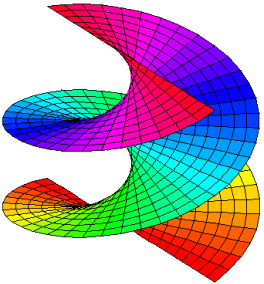
\includegraphics[scale=0.65]{picture/week7/helicoid.png}
        \caption{Helicoid}
    \end{subfigure}
    \begin{subfigure}{0.3\textwidth}
        \centering
        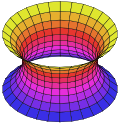
\includegraphics[scale=1.49]{picture/week7/catenoid.png}
        \caption{Catenoid}    
    \end{subfigure}
\end{figure}
\begin{enumerate}[(1)]
    \item Compute the \engordnumber{1} fundamental form of them.
    \[ I_H=\left(v^2+a^2\right)\dd u^2+\dd v^2\]
    \[I_C=\left(a^2\cosh^2\theta\right)\dd\varphi^2+
    \left(a^2\cosh^2\theta\right)\dd \theta^2\]
    \item Show that there is a parametrization on the helicoid, 
    \(\tilde{H}\left(\tilde{u},\tilde{v}\right)\), such that
    \[
        I_{\tilde{H}}=\left(a^2\cosh^2\tilde{v}\right)\dd \tilde{u}^2
        +\left(a^2\cosh^2\tilde{v}^2\right)\dd \tilde{v}^2    
    .\]
    (\(u=\tilde{u},v=a\sinh\tilde{v}\))
\end{enumerate}
\end{example}
\begin{remark}
    In both example 1 and example 3, we have seen that near a point, 
    the two surfaces considered have the same \engordnumber{1} 
    fundamental form
     (after a change of parametrization). Such property is called
      ``local isometry''. We'll make this definition more clear later.
\end{remark}

\(\bullet\)Application of the \engordnumber{1} fundamental form

\begin{enumerate}[(1)]
    \item Arclength of a curve on \(S\).
    
    Note that for a vector \(v\in \mathbb{R}^2\), \(I(v,v)=|v|^2\).
    Let \(\alpha(t)\colon (0,t)\to S\) be a curve in \(S\) and 
    \(\varphi \colon U\to S\), \((u,v)\mapsto\varphi (u,v)\) be a 
    local parametrization satisfying 
    \(\alpha(t)\in \varphi(U)\).
    \[
    \Rightarrow \alpha(t)=\varphi\left(u(t),v(t)\right) .   
    \]
    \[
      \Rightarrow\alpha'(t)=\varphi_u u'(t)+\varphi_v v'(t) .
    \]
    \[\Rightarrow \left|\alpha'(t)\right|^2=
    I\left(\alpha'(t),\alpha'(t)\right)=E u_t^2+2F u_t v_t +G v_t^2.\]
    The arclength of \(\alpha(t)\) is defined by 
    \[
        s(t)=\int_0^t  \left|\alpha'(t)\right|\dd t
        =\int_0^t \sqrt{E u_t^2+2F u_t v_t +G v_t^2}\dd t  .
    \]
    \[
        \Rightarrow \dd s=\sqrt{E u_t^2+2F u_t v_t +G v_t^2}\dd t.
    \]
    \[
        \Rightarrow\left(\dv{s}{t}\right)^2=E u_t^2+2F u_t v_t +G v_t^2.
    \]
    \[
        \Rightarrow \dd s^2=E \dd u^2+2F \dd u \dd v +G \dd v^2    .
    \]
    This explains the ``geometric meaning'' of \(I\), \ie\ it measures 
    the infinitesimal arclength.
    \item Angle between two curves intersecting at \(t_0\).
    
    Let \(\alpha\colon I\to S\), \(\beta\colon I\to S\) be two curves 
    on \(S\), \(\alpha(t_0)=\beta(\bar{t}_0)=p\in S\). 
    \begin{center}
        


\tikzset{every picture/.style={line width=0.75pt}} %set default line width to 0.75pt        

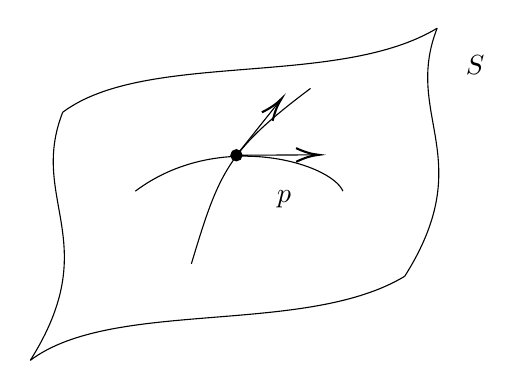
\begin{tikzpicture}[x=0.75pt,y=0.75pt,yscale=-1,xscale=1]
%uncomment if require: \path (0,300); %set diagram left start at 0, and has height of 300

%Curve Lines [id:da9909335153566519] 
\draw    (183,147) .. controls (223,117) and
 (315.4,135.5) .. (363.4,106.5) ;
%Curve Lines [id:da019275275220669075] 
\draw    (167.4,266.5) .. controls (203.4,209.5) and
 (166.4,189.5) .. (183,147) ;
%Curve Lines [id:da6995475257546488] 
\draw    (167.4,266.5) .. controls (207.4,236.5)
 and (299.8,255) .. (347.8,226) ;
%Curve Lines [id:da33316817877336646] 
\draw    (347.8,226) .. controls (383.8,169) and 
(346.8,149) .. (363.4,106.5) ;
%Shape: Circle [id:dp7349369009552857] 
\draw  [fill={rgb, 255:red, 0; green, 0; blue, 0 }  ,fill opacity=1 ] 
(264,167.7) .. controls (264,166.21) and (265.21,165) .. (266.7,165) 
.. controls (268.19,165) and (269.4,166.21) .. (269.4,167.7) .. 
controls (269.4,169.19) and (268.19,170.4) .. (266.7,170.4) .. 
controls (265.21,170.4) and (264,169.19) .. (264,167.7) -- cycle ;
%Curve Lines [id:da09382061994840107] 
\draw    (218,185) .. controls (258,155) and (312.4,171.5) .. (318,185) ;
%Curve Lines [id:da6577705388758515] 
\draw    (245,220) .. controls (258.4,175.5) and (262.4,165.5) .. (302.4,135.5) ;
%Straight Lines [id:da2459893691777446] 
\draw    (266.7,167.7) -- (287.15,142.06) ;
\draw [shift={(288.4,140.5)}, rotate = 128.58] [color={rgb, 255:red, 0; green, 0; blue, 0 }  ]
[line width=0.75]    (10.93,-3.29) .. controls (6.95,-1.4) and (3.31,-0.3) .. (0,0) .. controls 
(3.31,0.3) and (6.95,1.4) .. (10.93,3.29)   ;
%Straight Lines [id:da2821040919294362] 
\draw    (266.7,167.7) -- (304.4,167.51) ;
\draw [shift={(306.4,167.5)}, rotate = 179.71] [color={rgb, 255:red, 0; green, 0; blue, 0 }  ]
[line width=0.75]    (10.93,-3.29) .. controls (6.95,-1.4) and (3.31,-0.3) .. (0,0)
 .. controls (3.31,0.3) 
and (6.95,1.4) .. (10.93,3.29)   ;

% Text Node
\draw (376,118.4) node [anchor=north west][inner sep=0.75pt]    {$S$};
% Text Node
\draw (285,183.4) node [anchor=north west][inner sep=0.75pt]    {$p$};


\end{tikzpicture}
    \end{center}
    Define
        \[
            \cos \theta=\frac{\left\langle\alpha'(t_0),
            \beta'(\bar{t}_0)\right\rangle_{\mathbb{R}^3}}{
            \left|\alpha'(t_0)\right|\left|\beta'(\bar{t}_0) \right|}.
        \]
    \begin{question}
        Given a parametrization \(\varphi(u,v)\),
         we have two coordinate
         curve \(\varphi(u,v_0)\), \(\varphi(u_0,v)\). What's the angle 
         between them?
         \[u\text{-curve: }\alpha(t)=\varphi\left(u(t),c\right)
         \Rightarrow \alpha'(t)=\varphi_u u'.\]
         \[v\text{-curve: }\beta(t)=\varphi\left(c,v(t)\right)
         \Rightarrow \beta'(t)=\varphi_v v'.\] 
         \[
            \Rightarrow \cos \theta= 
            \frac{\left\langle \varphi_u u',\varphi_v v'\right\rangle}{
                \left|\varphi_u u'\right|\left|\varphi_v v'\right|
            }
            =\pm \frac{\left\langle\varphi_u,\varphi_v
            \right\rangle_{\mathbb{R}^3}}{\left|\varphi_u\right|
            \left|\varphi_v\right|}=\pm \frac{F}{\sqrt{EG}}  
         .\]
         In particular, we conclude that
         \[F=0\Leftrightarrow \text{Two coordinate curves are orthogonal,}\]
         and such parametrization is called an orthogonal parametrization.
         (e.g. For \(\mathbb{S}^2\), \((\theta,\varphi)\) and 
         the stereographic projection are two such parametrizations) 
    \end{question}
    \item (Surface) Area.
    
    Let \(S\) be a regular surface. Choose a parametrization 
    \(\varphi\colon U\to S\). Let \(Q\subset S\) be a bounded domain.
    Assume \(Q\subset \varphi(U)\), so \(\varphi^{-1}(Q)\subset U\) is 
    a bounded set in \(\mathbb{R}^2\).
    \begin{center}
\tikzset{every picture/.style={line width=0.75pt}} %set default line width to 0.75pt        

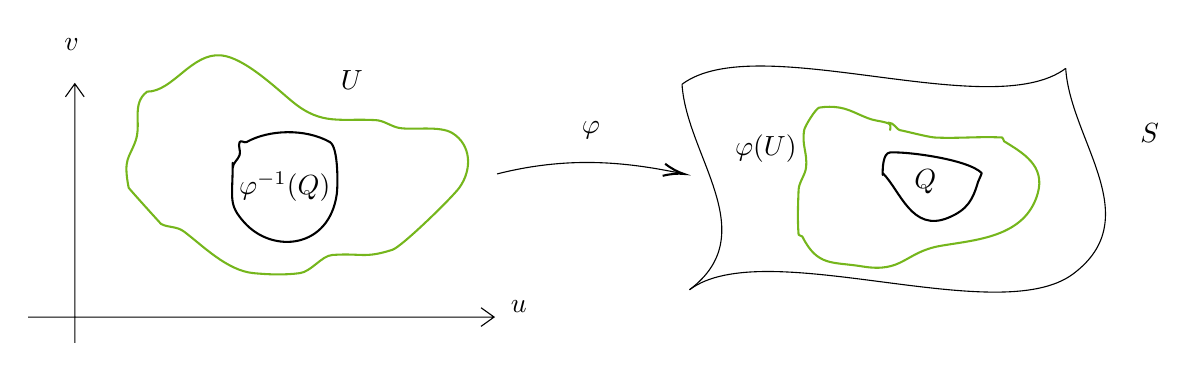
\begin{tikzpicture}[x=0.75pt,y=0.75pt,yscale=-0.9,xscale=0.9]
%uncomment if require: \path (0,300); %set diagram left start at 0, and has height of 300

%Shape: Axis 2D [id:dp30826843172023066] 
\draw  (67,239.62) -- (316.4,239.62)(91.94,114.71) -- (91.94,253.5) (309.4,234.62) -- (316.4,239.62)
 -- (309.4,244.62) (86.94,121.71) -- (91.94,114.71) -- (96.94,121.71)  ;
%Curve Lines [id:da2230443220096674] 
\draw [color={rgb, 255:red, 117; green, 182; blue, 28 }  ,draw opacity=1 ][line width=0.75] 
[line join = round][line cap = round]   (130.65,118.95) .. controls (122.05,125.38) and (127.75,136.1)
.. (124.46,145.32) .. controls (121.04,154.89) and (117.73,154.56) .. (120.74,170.31) .. controls (120.84,170.81) and (138.01,189.7) .. (138.08,189.74) .. controls (142.04,191.95) and (146.26,190.76) .. (150.46,193.9) .. controls (160.22,201.19) and (173.4,214.78) .. (187.61,216.11) .. controls (195.84,216.88) and (204.18,217.17) .. (212.38,216.11) .. controls (218.48,215.32) and (224.1,206.79) .. (229.72,206.39) .. controls (245.72,205.27) and (246.88,208.43) .. (261.91,203.62) .. controls (267,201.99) and (294.17,175.43) .. (297.82,170.31) .. controls (304.87,160.44) and (304.12,147.39) .. (294.11,141.16) .. controls (287.42,136.99) and (273.12,139.67) .. (265.63,138.38) .. controls (261.37,137.65) and (257.55,134.47) .. (253.25,134.22) .. controls (234.05,133.09) and (224.32,137.27) .. (208.67,124.5) .. controls (200.24,117.64) and (182.83,100.69) .. (170.28,99.52) .. controls (154.41,98.04) and (144.45,118.95) .. (130.65,118.95) -- cycle ;
%Curve Lines [id:da779384228982472] 
\draw [line width=0.75] [line join = round][line cap = round]   (176.47,157.04) .. controls (176.47,176.42) and (173.86,179.1) .. (182.66,188.96) .. controls (197.74,205.87) and (228.15,203.16) .. (232.19,173.69) .. controls (232.75,169.62) and (233.14,148.55) .. (228.48,145.93) .. controls (215.25,138.52) and (195.8,139.26) .. (183.9,145.93) .. controls (182.79,146.56) and (180.82,144.74) .. (180.18,145.93) .. controls (179.12,147.92) and (180.91,150.71) .. (180.18,152.87) .. controls (179.34,155.4) and (176.47,157.12) .. (176.47,159.81) ;
%Curve Lines [id:da4093176006038537] 
\draw    (417,115) .. controls (457,85) and (582.4,136.5) .. (622.4,106.5) ;
%Curve Lines [id:da8843839986108935] 
\draw    (421,225) .. controls (461,195) and (586.4,246.5) .. (626.4,216.5) ;
%Curve Lines [id:da3854765584435005] 
\draw    (421,225) .. controls (461,195) and (419.4,153.5) .. (417,115) ;
%Curve Lines [id:da6146348531460317] 
\draw    (626.4,216.5) .. controls (666.4,186.5) and (624.8,145) .. (622.4,106.5) ;
%Curve Lines [id:da8543149552748068] 
\draw [color={rgb, 255:red, 117; green, 182; blue, 28 }  ,draw opacity=1 ][line width=0.75] [line join = round][line cap = round]   (528.4,139.5) .. controls (528.4,138.5) and (528.85,137.39) .. (528.4,136.5) .. controls (527.93,135.57) and (522.09,134.61) .. (521.4,134.5) .. controls (514.38,133.33) and (508.52,128.69) .. (501.4,127.5) .. controls (497.78,126.9) and (494.02,126.9) .. (490.4,127.5) .. controls (488.74,127.78) and (482.76,137.32) .. (482.4,139.5) .. controls (480.99,147.95) and (484.21,151.37) .. (483.4,159.5) .. controls (483,163.53) and (479.56,167.46) .. (479.4,171.5) .. controls (479.09,179.49) and (478.76,187.53) .. (479.4,195.5) .. controls (479.46,196.24) and (481.07,195.83) .. (481.4,196.5) .. controls (489.58,212.86) and (497.61,209.87) .. (513.4,212.5) .. controls (535.53,216.19) and (535.97,204.88) .. (555.4,201.5) .. controls (574.04,198.26) and (600.67,197.05) .. (607.4,173.5) .. controls (611.7,158.44) and (599.25,151.66) .. (589.4,145.5) .. controls (588.77,145.1) and (589.14,143.54) .. (588.4,143.5) .. controls (576.42,142.85) and (564.38,144.11) .. (552.4,143.5) .. controls (548.93,143.32) and (537.92,140.4) .. (533.4,139.5) .. controls (532.08,139.24) and (530.49,135.5) .. (527.4,135.5) ;
%Curve Lines [id:da5437419917187927] 
\draw [line width=0.75] [line join = round][line cap = round]   (524.4,162.5) .. controls (533.93,172.03) and (540,194.41) .. (559.4,186.5) .. controls (570.03,182.17) and (572.69,176.55) .. (575.4,167.5) .. controls (575.66,166.65) and (577.6,162.7) .. (577.4,162.5) .. controls (570.13,155.23) and (537.95,150.97) .. (528.4,151.5) .. controls (524.33,151.73) and (524.4,160.76) .. (524.4,163.5) ;
%Curve Lines [id:da9563040601689965] 
\draw    (318,163) .. controls (358.57,152.71) and (390.12,157.31) .. (416.4,162.67) ;
\draw [shift={(418,163)}, rotate = 191.68] [color={rgb, 255:red, 0; green, 0; blue, 0 }  ][line width=0.75]    (10.93,-3.29) .. controls (6.95,-1.4) and (3.31,-0.3) .. (0,0) .. controls (3.31,0.3) and (6.95,1.4) .. (10.93,3.29)   ;

% Text Node
\draw (178.47,160.44) node [anchor=north west][inner sep=0.75pt]    {$\varphi ^{-1}( Q)$};
% Text Node
\draw (233,106.4) node [anchor=north west][inner sep=0.75pt]    {$U$};
% Text Node
\draw (540,159.4) node [anchor=north west][inner sep=0.75pt]    {$Q$};
% Text Node
\draw (444,140.4) node [anchor=north west][inner sep=0.75pt]    {$\varphi ( U)$};
% Text Node
\draw (661,134.4) node [anchor=north west][inner sep=0.75pt]    {$S$};
% Text Node
\draw (362,133.4) node [anchor=north west][inner sep=0.75pt]    {$\varphi $};
% Text Node
\draw (324,229.4) node [anchor=north west][inner sep=0.75pt]    {$u$};
% Text Node
\draw (85,89.4) node [anchor=north west][inner sep=0.75pt]    {$v$};


\end{tikzpicture}
    \end{center}
    Let's assume the boundary of \(Q\) is a differentiable curve with 
    singularities lying in a measure zero set.
\begin{definition}[Area of \(Q\)]
    \[Area(Q)=\iint_{\varphi(Q)} \left|\varphi_u\wedge 
    \varphi_v \right|\dd u\dd v \quad(\text{double integral in }
    \mathbb{R}^2).\]
    Here, we give the definition in terms of a ``parametrization''. 
    However, the area of \(Q\) is a number only depending on \(Q\)
    itself. We should check that our definition does not depend on 
    the parametrization.
\end{definition}
\textbf{Claim}: 
\textcolor{blue}{\(Area(Q)\) defined above is independent of the
choice of parametrizations.}
\begin{proof} (Left as exercise)

    Let \(\psi(\alpha,\beta)\colon V\to S\) be another parametrization. 
    Let \(H=\psi^{-1}\circ \varphi\) be the change of parametrization,
    \(H(u,v)=(\alpha,\beta)\)\(\Rightarrow\varphi =\psi \circ H\).
    We compute \(\iint_{\varphi(Q)} \left|\varphi_u\wedge 
    \varphi_v \right|\dd u\dd v\).

    By chain rule 
    \[
        \begin{pmatrix}
            \varphi_u\\ \varphi_v
        \end{pmatrix}=
        \pdv{(\alpha,\beta)}{(u,v)}\begin{pmatrix}
            \psi_\alpha\\
            \psi_\beta
        \end{pmatrix}    .
    \]
    \begin{align*}
        \Rightarrow \varphi_u\wedge\varphi_v&=
        \left(\alpha_u\beta_v\right)\psi_\alpha\wedge\psi_\beta+
        \left(\alpha_v\beta_u\right)\psi_\beta\wedge\psi_\alpha\\
        &=\left(\alpha_u\beta_v-\alpha_v\beta_u\right)
        \psi_\alpha\wedge\psi_\beta\\
        &=\det\left(\pdv{(\alpha,\beta)}{(u,v)}\right)
        \psi_\alpha\wedge\psi_\beta.
    \end{align*}
    \[\Rightarrow \left|
        \varphi_u\wedge \varphi_v 
    \right|=\left|\det\left(\pdv{(\alpha,\beta)}{(u,v)}\right)\right|
    \left|\psi_\alpha\wedge\psi_\beta\right|.\]
    
    On the other hand,
    \[
        \begin{pmatrix}
            \dd u\\ \dd v
        \end{pmatrix}
        =\pdv{(u,v)}{(\alpha,\beta)}\begin{pmatrix}
            \dd \alpha\\
            \dd \beta
        \end{pmatrix} .
    \]
    Thus, the change of infinitesimal area element is
    \[
        \dd u\dd v=\left|\dd u\wedge\dd v\right|=
        \left|\det \left(\pdv{(u,v)}{(\alpha,\beta)}\right)\right|
        \left|\dd\alpha\wedge\dd\beta\right|=
        \left|\det \left(\pdv{(u,v)}{(\alpha,\beta)}\right)\right|
        \dd\alpha\dd\beta.
    \]
    \[\Rightarrow \left|\varphi_u\wedge \varphi_v \right|
        \dd u\dd v=\left|\psi_\alpha\wedge\psi_\beta\right|\dd \alpha
        \dd \beta.
    \]
    \[\Rightarrow \iint \left|\varphi_u\wedge \varphi_v \right|
    \dd u\dd v=\iint \left|\psi_\alpha\wedge\psi_\beta\right|\dd \alpha
    \dd \beta.\]
\end{proof}
\begin{remark}
    By the \engordnumber{1} fundamental form 
    \[
        I=E(\dd u)^2+2F \dd u\dd v+G(\dd v)^2    
    \]
    \[\Rightarrow Area=\iint \left|\varphi_u\wedge \varphi_v \right|
    \dd u\dd v=\iint \sqrt{EG-F^2}\dd u\dd v.\]
\end{remark}
\end{enumerate}
\section{Gauss maps and the \texorpdfstring{\engordnumber{2}}{2nd} fundamental form}
\(\bullet\) Gauss maps.
\begin{question}
    \textcolor{blue}{How is a regular surface curved in \(\mathbb{R}^3\)}? 
\end{question}
\underline{\textbf{Recall}}: \(S\subset\mathbb{R}^3\) is an oriented
regular surface. 
\(\Rightarrow\) We can choose a unit vector field 
    \begin{align*}
        \vb{n}\colon S&\to \mathbb{S}^2(1)\\
        p&\mapsto \vb{n}_p,
    \end{align*}
is well-defined everywhere on \(S\). Moreover, \(\vb{n}\) is a
differentiable map with its image lying on the unit sphere, and we 
called the map to be the Gauss map. \(\vb{n}\) determines an 
orientation of \(S\).
\begin{center}
    


\tikzset{every picture/.style={line width=0.75pt}} %set default line width to 0.75pt        

\begin{tikzpicture}[x=0.75pt,y=0.75pt,yscale=-1,xscale=1]
%uncomment if require: \path (0,300); %set diagram left start at 0, and has height of 300

%Curve Lines [id:da28129415507356703] 
\draw    (100,110) .. controls (140,80) and (233.8,125) .. (267.4,89.5) ;
%Curve Lines [id:da9562883564686324] 
\draw    (59,172) .. controls (99,142) and (192.8,187) .. (226.4,151.5) ;
%Curve Lines [id:da748577885122705] 
\draw    (59,172) .. controls (72.4,131.5) and (99.4,129.5) .. (100,110) ;
%Curve Lines [id:da2562375766370064] 
\draw    (226.4,151.5) .. controls (217.4,127.5) and (250.4,106.5) .. (267.4,89.5) ;
%Shape: Parallelogram [id:dp8965230202175429] 
\draw   (145.82,117.5) -- (201.4,117.5) -- (177.58,145.5) -- (122,145.5) -- cycle ;
%Shape: Circle [id:dp3509817579048975] 
\draw  [fill={rgb, 255:red, 0; green, 0; blue, 0 }  ,fill opacity=1 ] (161.7,131.5) .. controls (161.7,130.01) and (162.91,128.8) .. (164.4,128.8) .. controls (165.89,128.8) and (167.1,130.01) .. (167.1,131.5) .. controls (167.1,132.99) and (165.89,134.2) .. (164.4,134.2) .. controls (162.91,134.2) and (161.7,132.99) .. (161.7,131.5) -- cycle ;
%Straight Lines [id:da4477857542457926] 
\draw    (164.4,131.5) -- (163.44,81.5) ;
\draw [shift={(163.4,79.5)}, rotate = 88.9] [color={rgb, 255:red, 0; green, 0; blue, 0 }  ][line width=0.75]    (10.93,-3.29) .. controls (6.95,-1.4) and (3.31,-0.3) .. (0,0) .. controls (3.31,0.3) and (6.95,1.4) .. (10.93,3.29)   ;
%Shape: Axis 2D [id:dp2767501351977306] 
\draw  (465,150) -- (565,150)(475,60) -- (475,160) (558,145) -- (565,150) -- (558,155) (470,67) -- (475,60) -- (480,67)  ;
%Straight Lines [id:da9011328855757925] 
\draw    (475,150) -- (407.83,216.1) ;
\draw [shift={(406.4,217.5)}, rotate = 315.46] [color={rgb, 255:red, 0; green, 0; blue, 0 }  ][line width=0.75]    (10.93,-3.29) .. controls (6.95,-1.4) and (3.31,-0.3) .. (0,0) .. controls (3.31,0.3) and (6.95,1.4) .. (10.93,3.29)   ;
%Shape: Circle [id:dp28714049477405257] 
\draw  [color={rgb, 255:red, 144; green, 19; blue, 254 }  ,draw opacity=1 ] (431.8,150) .. controls (431.8,126.14) and (451.14,106.8) .. (475,106.8) .. controls (498.86,106.8) and (518.2,126.14) .. (518.2,150) .. controls (518.2,173.86) and (498.86,193.2) .. (475,193.2) .. controls (451.14,193.2) and (431.8,173.86) .. (431.8,150) -- cycle ;
%Straight Lines [id:da45439583119974114] 
\draw    (475,150) -- (439.08,126.59) ;
\draw [shift={(437.4,125.5)}, rotate = 33.09] [color={rgb, 255:red, 0; green, 0; blue, 0 }  ][line width=0.75]    (10.93,-3.29) .. controls (6.95,-1.4) and (3.31,-0.3) .. (0,0) .. controls (3.31,0.3) and (6.95,1.4) .. (10.93,3.29)   ;
%Curve Lines [id:da1330380081969107] 
\draw    (283,139) .. controls (322.4,109.45) and (349.58,123.08) .. (381.54,138.3) ;
\draw [shift={(383,139)}, rotate = 205.43] [color={rgb, 255:red, 0; green, 0; blue, 0 }  ][line width=0.75]    (10.93,-3.29) .. controls (6.95,-1.4) and (3.31,-0.3) .. (0,0) .. controls (3.31,0.3) and (6.95,1.4) .. (10.93,3.29)   ;

% Text Node
\draw (190,136.4) node [anchor=north west][inner sep=0.75pt]    {$T_{p} S$};
% Text Node
\draw (158,56.4) node [anchor=north west][inner sep=0.75pt]    {$\vb{n}$};
% Text Node
\draw (147.82,120.9) node [anchor=north west][inner sep=0.75pt]    {$p$};
% Text Node
\draw (262,70.4) node [anchor=north west][inner sep=0.75pt]    {$S$};
% Text Node
\draw (390,214.4) node [anchor=north west][inner sep=0.75pt]    {$x$};
% Text Node
\draw (577,141.4) node [anchor=north west][inner sep=0.75pt]    {$y$};
% Text Node
\draw (469,38.4) node [anchor=north west][inner sep=0.75pt]    {$z$};
% Text Node
\draw (517,93.4) node [anchor=north west][inner sep=0.75pt]    {$\mathbb{S}^{2}$};
% Text Node
\draw (418,102.4) node [anchor=north west][inner sep=0.75pt]   {$\vb{n}_{p}$};
% Text Node
\draw (326,98.4) node [anchor=north west][inner sep=0.75pt]    {$\vb{n}$};


\end{tikzpicture}
\end{center}
Let \(\varphi \colon U\to S\) be a local parametrization near 
\(p\in S\), then 
\[
    \vb{n}=\frac{\varphi_u\wedge\varphi_v}{
        \left|\varphi_u\wedge\varphi_v\right|}.    
\]
Let's compute the differential of the Gauss map at \(p\).
\[
    \dd\vb{n}_p\colon T_p S\to T_{\vb{n}_p}\mathbb{S}^2    .
\]
\(\forall v\in T_p S\), let \(\alpha(s)\) be the curve on \(S\)
such that \(\alpha(0)=p\), \(\alpha'(0)=v\).
\[
    \Rightarrow
    \dd\vb{n}_p(v)=\left.\dv{s}\right|_{s=0}\vb{n}\left(\alpha(s)\right)
    (\text{changing rate of the Gauss map at }p
    \text{ along direction }v).
\]
Note \(\left\langle\vb{n}\left(\alpha(s)\right),
\vb{n}\left(\alpha(s)\right)\right\rangle=1\), taking derivation at 
\(s=0\): 
\[
\left\langle\left.\dv{s}\right|_{s=0}\vb{n}\left(\alpha(s)\right),
\vb{n}_p \right\rangle=0.
\]
\[
    \Rightarrow 
    \dd\vb{n}_p(v)=\left.\dv{s}\right|_{s=0}\vb{n}\left(\alpha(s)\right)
    \in T_p S.
\]
\begin{definition}[The \engordnumber{2} fundamental form]
    \hfill
    \begin{itemize}
        \item \(\forall v\in T_p S\), the \engordnumber{2} fundamental
        form 
        \[\II_p(v,v)=
        -\left\langle \dd\vb{n}_p(v),
        v\right\rangle_{\mathbb{R}^3}\footnotemark.\]
        \footnotetext{Thus, \(\dd\vb{n}_p\colon T_p S\to T_p S\) 
        is a linear map, which is the directional derivation of 
        \(\vb{n}\) along a tangent direction of \(S\).}
        \item More generally \(\forall v,w\in T_p S\), 
        \[
            \II_p\colon T_p S\times T_p S\to T_p \mathbb{R}
        \]
         \[   (v,w)\mapsto \II_p(v,w)=-\left\langle
                \dd\vb{n}_p(v),w\right\rangle_{\mathbb{R}^3}.
        \]

    \end{itemize}
    \(-\dd \vb{n}_p\) is also called the shape operator.
\end{definition}
Before we explore \(\II_p\), let's compute the Gauss map's
differential.

\(\bullet\) Let \(\varphi(u,v)\) be a local parametrization. 
Any curve on \(S\) has parametrization
\[  
    \alpha(t)=\varphi\left(u(t),v(t)\right)=
    \left(x\left(u(t),v(t)\right),
        y\left(u(t),v(t)\right),
        z\left(u(t),v(t)\right)\right).
\]
\[\Rightarrow \alpha'(0)=\varphi_u u'(0)+\varphi_v v'(0).\]
\begin{align*}
    \dd \vb{n}_p\left(\alpha'(0)\right)
    &=\left.\dv{t}\right|_{t=0}\vb{n}\left(\alpha(t)\right)\\
    &=\left.\dv{t}\right|_{t=0}\vb{n}
    \left(x\left(u(t),v(t)\right),
        y\left(u(t),v(t)\right),
        z\left(u(t),v(t)\right)\right)\\
    &=\left(\vb{n}_x x_u+\vb{n}_y y_u+\vb{n}_z z_u\right)u'(0)
    +\left(\vb{n}_x x_v+\vb{n}_y y_v+\vb{n}_z z_v\right)v'(0)\\    
    &=\vb{n}_u u'(0)+\vb{n}_v v'(0).
\end{align*}
On the other hand, by the linearity of \(\dd \vb{n}_p\), 
\[
    \dd\vb{n}_p\left(\alpha'(0)\right)=u'(0)\dd \vb{n}_p
    \left(\varphi_u\right)+v'(0)\dd\vb{n}_p \left(\varphi_v\right).    
\]
\[
    \Rightarrow
    \begin{cases}
        \dd\vb{n}_p\left(\vphi_u\right)=\vb{n}_u,\\
        \dd\vb{n}_p\left(\vphi_v\right)=\vb{n}_v.
    \end{cases}
\]
\begin{align*}
    \left\langle \dd\vb{n}_p\left(\vphi_u\right),\vphi_u
    \right\rangle
    &=\left\langle\vb{n}_u,\vphi_u\right\rangle=
    \pdv{u}\underbrace{\left\langle\vb{n},\vphi_u\right\rangle}_{=0}
    -\left\langle\vb{n},\vphi_{uu}\right\rangle\\
    \left\langle \dd\vb{n}_p\left(\vphi_u\right),\vphi_v
    \right\rangle
    &=\left\langle\vb{n}_u,\vphi_v\right\rangle\\
    &=\pdv{u}\underbrace{\left\langle\vb{n},\vphi_v\right\rangle}_{=0}
    -\left\langle\vb{n},\vphi_{vu}\right\rangle\\
    &=-\left\langle\vb{n},\vphi_{vu}\right\rangle\\
    \left\langle \dd\vb{n}_p\left(\vphi_v\right),\vphi_u
    \right\rangle
    &=\left\langle\vb{n}_v,\vphi_u\right\rangle\\
    &=-\left\langle\vb{n},\vphi_{uv}\right\rangle
    (\text{Note that }\vphi_{uv}=\vphi_{vu}\text{ since }
    \vphi\text{ is smooth})\\
    \left\langle \dd\vb{n}_p\left(\vphi_v\right),\vphi_v
    \right\rangle
    &=\left\langle\vb{n}_v,\vphi_v\right\rangle
    =-\left\langle \vb{n}, \vphi_{vv}\right\rangle.
\end{align*}
Hence, we conclude that: 
\begin{theorem}
    \(\II_p(v,w)=\II_p(w,v)\), \ie\ 
    \(\II_p\) is symmetric in \(v\), \(w\), and
    \(\II_p\) is a bilinear form. 
\end{theorem}
\begin{remark}
    \hfill
    \begin{enumerate}[(1)]
        \item From the computation above, we see that 
        \(\dd\vb{n}_p\) is self-adjoint, \ie\ 
        \(\left\langle \dd\vb{n}_p(v),w\right\rangle=
        \left\langle v, \dd\vb{n}_p(w)\right\rangle
        \).
        \item The \engordnumber{2} fundamental form can be also 
        defined as 
        \[\II_p(v,v)=\left\langle\vb{n}_p,\alpha''(0)\right\rangle,\]
        where \(\alpha\) is a curve with \(\alpha'(0)=v\).
    \end{enumerate}
\end{remark}
\begin{exercise}
    Check that this definition coincides with the previous one.
\end{exercise}
\begin{proof}
    Along the curve \(\alpha(t)\in S\), \(\left\langle
    \vb{n}\left(\alpha(t)\right),\alpha'(t)\right\rangle=0\).
    Therefore, 
    \begin{align*}
        0&=\dv{t}\left\langle\vb{n}\left(\alpha(t)\right),\alpha'(t)
        \right\rangle\\
        &= \left\langle \dd\vb{n}_{\alpha(t)}\left(\alpha'(t)
        ,\alpha'(t)\right)\right\rangle+\left\langle
         \vb{n}\left(\alpha(t)\right),\alpha''(t)\right\rangle.
    \end{align*}
\end{proof}
Just as the \engordnumber{1} fundamental form, we write \(\II\) as 
\[
    \II_p=e\dd u^2+2f\dd u\dd v+g\dd v^2,
\]
where 
\begin{align*}
    e&=-\left\langle \dd\vb{n}_p\left(\varphi_u\right),\varphi_u\right\rangle
    =-\left\langle\vb{n}_u,\varphi_u\right\rangle=\left\langle
        \vb{n},\varphi_{uu}\right\rangle\\
    f&=-\left\langle \dd\vb{n}_p\left(\varphi_u\right),\varphi_v\right\rangle
    =-\left\langle\vb{n}_u,\varphi_v\right\rangle=\left\langle
        \vb{n},\varphi_{uv}\right\rangle\\
        (&=-\left\langle \dd\vb{n}_p\left(\varphi_v\right),\varphi_u
        \right\rangle=-\left\langle\vb{n}_v,\varphi_u\right\rangle
        =\left\langle\vb{n},\varphi_{vu}\right\rangle)\\
        g&=-\left\langle \dd\vb{n}_p\left(\varphi_v\right),\varphi_v
        \right\rangle=-\left\langle\vb{n}_v,\varphi_v
        \right\rangle=\left\langle\vb{n},\varphi_{vv}\right\rangle
\end{align*}
\(\bullet\) Weingarten equations (linear representation of \(\dd\vb{n}\)
in \(\{\varphi_u,\varphi_v\}\))

We have seen \(\dd{\vb{n}}_p\colon T_p S\to T_{\vb{n}_p}\mathbb{S}^2\)
has image actually lying in \(T_p S=\Span\left\{\varphi_u,
\varphi_v\right\}\) in terms of a local parametrization \(\varphi(u,v)\).
\[
    \Rightarrow \begin{cases}
        \dd\vb{n}_p\left(\varphi_u\right)=a_{11}\varphi_u+a_{12}\varphi_v\\
        \dd\vb{n}_p\left(\varphi_v\right)=a_{21}\varphi_u+a_{22}\varphi_v
    \end{cases}
    \ie\ \begin{cases}
        \vb{n}_u=a_{11}\varphi_u+a_{12}\varphi_v\\
        \vb{n}_v=a_{21}\varphi_u+a_{22}\varphi_v
    \end{cases}
\]
We would like to find out the matrix \(\begin{pmatrix}
    a_{11}&a_{12}\\
    a_{21}&a_{22}
\end{pmatrix}\).

Recall that 
\[
    I_p=E\dd u^2+2F \dd u\dd v+G\dd v^2,
\]
where
\[
    E=\left\langle\varphi_u,\varphi_u\right\rangle,
    F=\left\langle\varphi_u,\varphi_v\right\rangle,
    G=\left\langle\varphi_v,\varphi_v\right\rangle.    
\]
Now we consider the matrix 
\[
    \begin{pmatrix}
        \vb{n}_u\\
        \vb{n}_v
    \end{pmatrix}
    \begin{pmatrix}
        \varphi_u &\varphi_v
    \end{pmatrix}=
    \begin{pmatrix}
        \left\langle\vb{n}_u,\varphi_u\right\rangle&
        \left\langle\vb{n}_u,\varphi_v\right\rangle\\
        \left\langle\vb{n}_v,\varphi_u\right\rangle&
        \left\langle\vb{n}_v,\varphi_v\right\rangle
    \end{pmatrix}.    
\]
On the one hand, the R.H.S. is 
\[
    \begin{pmatrix}
    -e&-f\\
    -f&-g
    \end{pmatrix}=-
    \begin{pmatrix}
        e&f\\
        f&g
    \end{pmatrix}.
\]
On the other hand,
\begin{align*}
    \text{R.H.S.}&=\begin{pmatrix}
        a_{11}E+a_{12}F&
        a_{11}F+a_{12}G\\
        a_{21}E+a_{22}F&
        a_{21}F+a_{22}G
    \end{pmatrix}\\
    &=\begin{pmatrix}
        a_{11}&a_{12}\\
        a_{21}&a_{22}
    \end{pmatrix}
    \begin{pmatrix}
        E&F\\
        F&G
    \end{pmatrix}.
\end{align*}
\[
    \Rightarrow 
    -\underbrace{\begin{pmatrix}
        e&f\\
        f&g
    \end{pmatrix}}_{\II}
    =
    \begin{pmatrix}
        a_{11}&a_{12}\\
        a_{21}&a_{22}
    \end{pmatrix}
    \underbrace{\begin{pmatrix}
        E&F\\
        F&G
    \end{pmatrix}}_{I}.
\]
\begin{align*}
    \Rightarrow
    \begin{pmatrix}
        a_{11}&a_{12}\\
        a_{21}&a_{22}
    \end{pmatrix}
    &=-\begin{pmatrix}
        e&f\\
        f&g
    \end{pmatrix}
    \begin{pmatrix}
        E&F\\
        F&G
    \end{pmatrix}^{-1}\\
    &=-\begin{pmatrix}
        e&f\\
        f&g
    \end{pmatrix}
    \frac{1}{\det}\begin{pmatrix}
        G&-F\\
        -F&E
    \end{pmatrix}\\
    &=-\frac{1}{EG-F^2}\begin{pmatrix}
        e&f\\
        f&g
    \end{pmatrix}
    \begin{pmatrix}
        G&-F\\
        -F&E
    \end{pmatrix}\\
    &=\frac{1}{EG-F^2}\begin{pmatrix}
        fF-eG& e F-fE\\
        gF-fG& fF-gE
    \end{pmatrix}\tag{\(\ast \)}.
\end{align*}
The Weingarten equation is \(\dd\vb{n}_p\sim \begin{pmatrix}
    a_{11}&a_{12}\\
    a_{21}&a_{22}
\end{pmatrix}\),
\ie\ 
\[
    \begin{pmatrix}
        \vb{n}_u\\
        \vb{n}_v
    \end{pmatrix}=
    \begin{pmatrix}
        a_{11}&a_{12}\\
        a_{21}&a_{22}
    \end{pmatrix}
    \begin{pmatrix}
        \varphi_u\\
        \varphi_v
    \end{pmatrix},
\]
with \(\begin{pmatrix}
    a_{11}&a_{12}\\
    a_{21}&a_{22}
\end{pmatrix}\) defined in (\(\ast\)).

\begin{itemize}
    \item[{\Large\textcolor{red}{\textbf{!}}}]
    For a regular surface \(S\subset \mathbb{R}^3\), 
    if we know the local parametrization \(\varphi(u,v)\) near 
    a point \(p\), then 
    \[
        I_p=E\dd u^2+2F \dd u\dd v+G\dd v^2,
    \]
    and 
    \[
        \II_p=e\dd u^2+2f\dd u\dd v+g\dd v^2,
    \]
    are fully understood with
    \[
        \begin{pmatrix}
            E&F\\
            F&G
        \end{pmatrix}
        =\begin{pmatrix}
            \left\langle\varphi_u,\varphi_u\right\rangle
            &
            \left\langle\varphi_u,\varphi_v\right\rangle
            \\
            \left\langle\varphi_v,\varphi_u\right\rangle
            &
            \left\langle\varphi_v,\varphi_v\right\rangle
        \end{pmatrix},
    \]
    and 
    \[
        \begin{pmatrix}
            e&f\\
            f&g
        \end{pmatrix}
        =\begin{pmatrix}
            \left\langle\varphi_{uu},\vb{n}\right\rangle&
            \left\langle\varphi_{uv},\vb{n}\right\rangle\\
            \left\langle\varphi_{vu},\vb{n}\right\rangle &
            \left\langle\varphi_{vv},\vb{n}\right\rangle
        \end{pmatrix}.
    \]
\end{itemize}
\begin{example}
    \begin{enumerate}[(1)]
        \hfill
        \item Plane: \(Ax +B y+C z+D=0 \)
        \[\vb{n}=\frac{(A,B,C)}{\sqrt{A^2+B^2+C^2}}\]
        is a constant map. Thus, 
        \(
            \dd\vb{n}=0    
        \) and \(\II(v,v)=-\left\langle \dd\vb{n}(v),v\right\rangle=0\).
        \item \(\mathbb{S}^2(1)=\{x^2+y^2+z^2=1\}\).
        At point \((x,y,z)\), the unit normal vector field is 
        \(\vb{n}_{\pm}=\pm (x,y,z)\), where \(\vb{n}_+\) means 
        the outer normal vector, and \(\vb{n}_-\) the inner normal 
        vector.

        Let's consider \(\vb{n}_-=-(x,y,z)\), let \(\alpha(t)=\left(
        x(t),y(t),z(t)\right)\) be a curve on \(\mathbb{S}^2\), then 
        \[
            \dd\vb{n}_-\left(\alpha'(t)\right)
            =\dv{t}\vb{n}_- \left(\alpha(t)\right)
            =-\dv{t}\left(x(t),y(t),z(t)\right)
            =-\alpha'(t)    
        .\]
        \[\Rightarrow
            \II\left(\alpha'(t),\alpha'(t)\right)
            =-\left\langle \dd\vb{n}_-\left(\alpha'(t)\right)
            \right\rangle=\left\langle\alpha'(t),\alpha'(t)
            \right\rangle=\left|\alpha'(t)\right|^2\ge 0.
        \]
        If we take \(\vb{n}_+\), then 
        \[\II\left(\alpha'(t),\alpha(t)\right)=
        -\left|\alpha'(t)\right|^2\le 0.\]
        \underline{Hence}, sign of the \engordnumber{2} fundamental form
    depends on the choice of orientation (\ie\ the unit normal).
    \item Helicoid (in which every point looks like a saddle point).
    \[H(u,v)=(v\cos u,v\sin u,a u)\]
    \[H_u=(-v\sin u,v\cos u,a),\quad H_v=(\cos u,\sin u,0).\]
    \[H_{uu}=(-v\cos u,-v\sin u,0),H_{uv}=(-\sin u,\cos u,0),
    H_{vv}=(0,0,0).
    \]
    \[
        \vb{n}=\left(-\frac{a\sin u}{\sqrt{a^2+v^2}},
        \frac{a\cos u}{\sqrt{a^2+v^2}},
        -\frac{v}{\sqrt{a^2+v^2}}
        \right).    
    \]
    \[
        \II=\frac{2a}{\sqrt{a^2+v^2}}\dd u\dd v    ,
    \]
    \ie\ 
    \[
        \begin{pmatrix}
            e&f\\
            f&g
        \end{pmatrix}=\begin{pmatrix}
            0&\frac{2a}{\sqrt{a^2+v^2}}\\
            \frac{2a}{\sqrt{a^2+v^2}}&0
        \end{pmatrix},\quad
        \lambda=\pm \frac{a}{\sqrt{a^2+v^2}}\text{ indefinite}.
    \]
    \item Cylinder. \(x^2+y^2=1\)
    \[
        c(\theta,v)=(\cos \theta,\sin\theta,v).    
    \]
    \[
        c_\theta=(-\sin \theta,\cos \theta,0),\quad
        c_v=(0,0,1).    
    \]
    \[
        \vb{n}_+=(\cos\theta,\sin\theta,0)(\text{the outer normal}),    
    \]
    \[
        \vb{n}_-=(-\cos\theta,-\sin\theta,0)(\text{the inner normal}).
    \]
    \[
        c_{\theta\theta}=(-\cos \theta,-\sin\theta,0),\quad
        c_{\theta v}=(0,0,0),\quad
        c_{vv}=(0,0,0).    
    \]
    \[\Rightarrow \II_{\vb{n}_-}=d \theta^2\sim \begin{pmatrix}
        1&0\\0&0
    \end{pmatrix}.\]
    \end{enumerate}  
\end{example}
\begin{remark}
    The cylinder and the plane have the same \engordnumber{1} fundamental
    form, but different \engordnumber{2} fundamental form.
\end{remark}
\section{Geometric meaning of the \texorpdfstring{\engordnumber{2}}{2nd} fundamental form and curvatures}
\underline{Recall}: \begin{itemize}
    \item Gauss map \[\vec{N}\colon S\to \mathbb{S}^2(1),\]
    \[p\mapsto \vec{N}_p.\]
    \item \(d \vec{N}_p\colon T_p S\to T_{\vec{N}(p)}\mathbb{S}^2(1)
    \simeq T_p S\).
    \item \(\forall v \in T_p S\), \(\II(v,v)=-\left\langle d 
    \vec{N}_p(v),v
    \right\rangle=\left\langle \vec{N}_p,
    \alpha''(0)\right\rangle\), where
    \(\alpha\) is a curve with \(\alpha(0)=p\), \(\alpha'(0)=v\).
\end{itemize}
(Note that at \(p\) along direction \(v\), there are indefinitely
many, curves passing through \(p\) with tangent vector \(v\), each
can be obtained by using a plane containing \(p,v\) to intersect with
\(S\)). However, \(\II(v,v)\) only depends on \(\alpha'(0)=v\).

\underline{Goal}: Understanding how \engordnumber{2} fundamental 
form reflects the surface is curved locally near a point.
\subsection{Normal curvature}
    
    Let \(\alpha(s)\) be a regular curve parametrized by the arclength In
    \(S\). 
    \[
        \Rightarrow \alpha'(s)=t(s),\quad \left|\alpha'(s)\right|=1
    \]
    \[
        \alpha''(s)=t'(s)=k(s)\vb{n}(s),\quad k(s):\text{curvature of
        }\alpha(s),\quad\vb{n}:\text{unit normal vector of }\alpha(s)
    \]
\begin{align*}
    \left\langle\alpha''(s),\vec{N}\left(\alpha(s)\right)\right\rangle
    &=\dv{s}\langle\underbrace{\alpha'(s)}_{\in T_{\alpha(s)}S}
    \vec{N}\left(\alpha(s)\right)\rangle-\left\langle
        \alpha'(s),\dv{s}\vec{N}\left(\alpha(s)\right)
    \right\rangle\\
    &=-\left\langle\alpha'(s),d\vec{N}_{\alpha(s)}\left(\alpha'(s)
    \right)\right\rangle\\
    &=\II\left(\alpha'(s),\alpha'(s)\right)
\end{align*}
On the other hand, 
\[
    \left\langle\alpha''(s),\vec{N}(\alpha(s))\right\rangle    
    =\left\langle k(s) \vb{n}(s),\vec{N}(s)\right\rangle
    =k(s)\cos \theta.
\]
This is the projection of ``curvature'' of \(\alpha(s)\) on the normal
vector of the surface. We call the value
\[
    k_{\vb{n}}=k(s)\cos \theta
\]
to be the ``normal curvature of curve \(\alpha(s)\)''.

Hence, the \engordnumber{2} fundamental form
\[
    \II\left(\alpha'(s),\alpha'(s)\right)    
    =\text{normal curvature of }\alpha(s)=k_{\vb{n}}.
\]
But \(\II\left(\alpha'(s),\alpha'(s)\right)\) only depends on 
\(\alpha'(s)\) but not a particular curve. Hence, at \(p\in S\), 
all curves passing through \(p\) with the same unit tangent vector
\(v\) have the same normal curvature. A canonical choice of
such curve is called the ``normal section'' which is a curve 
obtained by intersecting the plane \(\Span\{\underbrace{v}_{unit},N\}\)
with \(S\)
\[
    \Rightarrow k_{\vb{n}}=\pm \text{curvature of normal section along
    direction }v.
\]
\[
    \Rightarrow \II(v,v)= \pm \text{curvature of normal section along
    direction }v.   
\]
\begin{exercise}
    Compute \(k_{\vb{n}}\) in a local parametrization.

    Let \(\alpha(s)=\varphi\left(u(s),v(s)\right)\), 
    \(\alpha'(s)=\varphi_u u'(s)+\varphi_v v'(s)\), where \(s\)
    is the arclength parameter. Then, 
    \[
        \alpha''(s)=\varphi_{uu}\left(u'(s)\right)^2 +2\varphi_{uv}
        u'(s)v'(s)+\varphi_{vv}\left(v'(s)\right)^2
        +\underbrace{\varphi_u u''(s)+\varphi_v v''(s)}_{tangential}.
    \]
    \begin{align*}
        &\left\langle \alpha''(s),
        \vec{N}\left(\alpha(s)\right)\right\rangle\\
        =&\left\langle \varphi_{uu},\vec{N}\right\rangle
        \left(u'(s)\right)^2 +2\left\langle\varphi_{uv},
        \vec{N}\right\rangle u'(s)v'(s)+\left\langle
        \varphi_{vv},\vec{N}\right\rangle\left(v'(s)\right)^2\\
        =&e \left(u'(s)\right)^2+2fu'(s)v'(s)+g\left(v'(s)\right)^2
    .\end{align*}
    Therefore, 
    \[
        k_{\vb{n}}\left(\alpha'(s)\right)=
        e \left(u'(s)\right)^2+2fu'(s)v'(s)+g\left(v'(s)\right)^2.
    \]
    It's also interesting to obtain \(k_{\vb{n}}\) in an 
    arbitrary parametrization. Let \(\alpha(\tau)\) be some parameter,
    \[
        \Rightarrow
        S=\left(\tau\right)    \int_0^\tau \left|\alpha'(\tau)\right|
        \dd \tau
        ,\quad \tau'(s)=\frac{1}{\left|\alpha'(\tau)\right|}.
    \]
    \begin{align*}
        \alpha'(s)&=\alpha'(\tau)\tau'(s),\\
        \alpha''(s)&=\alpha''(\tau)\left(\tau'(s)\right)^2+
        \alpha'(\tau)\tau''(s).
    \end{align*}
    \begin{align*}
        \left\langle\alpha''(s),\vec{N}\left(\alpha(\tau)\right)
        \right\rangle
        &=\left\langle\alpha''(\tau),\vec{N}\left(\alpha(\tau)\right)
        \right\rangle\left(\tau'(s)\right)^2\\
        &=\frac{\II\left(\alpha'(\tau),\alpha'(\tau)\right)}{
            I\left(\alpha'(\tau),\alpha'(\tau)\right)
        }.
    \end{align*}
    \[
        \therefore   k_{\vb{n}}\left(\alpha'(\tau)\right)
        =\frac{\II\left(\alpha'(\tau),\alpha'(\tau)\right)}{
            I\left(\alpha'(\tau),\alpha'(\tau)\right)
        }.
    \]
\end{exercise}
\begin{itemize}
    \item[{\Large\textcolor{red}{\textbf{!}}}] The normal curvature
    along direction \(v\) is \(\II(v,v)\) tells us that how the 
    surface is curved along direction \(v\) at \(p\).
\end{itemize}
\begin{example}\label{normal curvature-sphere}
    Sphere: \(x^2+y^2+z^2=1\).
\end{example}

Normal sections are the great circles of radius \(1\).
         \[\therefore \II(v,v)=1,\quad\forall |v|=1.\]
        \begin{center}
            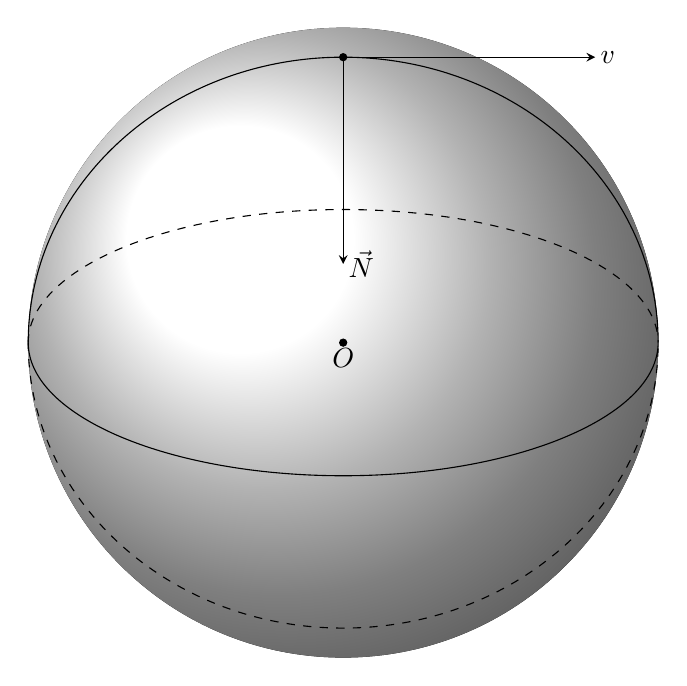
\begin{tikzpicture}[scale=2]%抄的知乎:https://zhuanlan.zhihu.com/p/494100190
                \pgfmathsetmacro{\R}{2};
                \pgfmathsetmacro{\AngleGamma}{25}
                \tikzset{%>=latex, % option for nice arrows
                    inner sep=0pt,%
                    outer sep=2pt,%
                     mark coordinate/.style=
                     {inner sep=0pt,outer sep=0pt,minimum size=3pt,
                    fill=black,circle}%
                        }
            \newcommand\LongitudePlane[3][current plane]{
            \tikzset{#1/.estyle={cm={cos(#3),sin(#3)*sin(#2),0,cos(#2),(0,0)}}}}
            \newcommand\DrawLongitude[3][\AngleGamma]{
            \LongitudePlane{#1}{#3}
            \tikzset{current plane/.prefix style={scale=#2}}
                             % angle of "visibility"
            \pgfmathsetmacro\angVis{atan(sin(#3)*cos(#1)/sin(#1))} %
            \draw[current plane,thin,black] 
            (\angVis:1) arc (\angVis:\angVis+180:1);
            \draw[current plane,thin,dashed] 
            (\angVis-180:1) arc (\angVis-180:\angVis:1);
            }
            \newcommand\LatitudePlane[3][current plane]{
  \pgfmathsetmacro\yshift{cos(#2)*sin(#3)}
  % 下面 cm 的最后一个参数不能出现乘法,所以定义了 yshift
  \tikzset{#1/.estyle={cm={cos(#3),0,0,cos(#3)*sin(#2),(0,\yshift)}}}
}
% 参数1:【可选】极点的倾斜角,默认 `\AngleGamma`
% 参数2:地球半径
% 参数3:维度(北正南负)
\newcommand\DrawLatitude[3][\AngleGamma]{
  \LatitudePlane{#1}{#3}
  \tikzset{current plane/.prefix style={scale=#2}}
  \pgfmathsetmacro\sinVis{sin(#3)/cos(#3)*sin(#1)/cos(#1)}
  % angle of "visibility"
  \pgfmathsetmacro\angVis{asin(min(1,max(\sinVis,-1)))}
  \draw[current plane,thin,black] (\angVis:1) arc (\angVis:-\angVis-180:1);
  \draw[current plane,thin,dashed] (180-\angVis:1) arc (180-\angVis:\angVis:1);
}        
	        {
                \fill[ball color=white!10] (0,0) circle (\R);
                \coordinate[mark coordinate] (N) at (0,{\R*cos(\AngleGamma)});
                \coordinate[mark coordinate] (O) at (0,0);
                \node[below] at (O) {\(O\)};
                \DrawLongitude{\R}{0};
                \DrawLatitude{\R}{0};
                \draw[->,>=stealth]
                (0,{\R*cos(\AngleGamma)})to({\R*0.8},{\R*cos(\AngleGamma)})
                node[right]{\(v\)};
                \draw[->,>=stealth]
                (0,{\R*cos(\AngleGamma)})to(0,{\R*0.25})
                node[right]{\(\vec{N}\)};
            }
            \end{tikzpicture}
        \end{center}
     \begin{example}\label{normal curvature-cylinder}
         Cylinder: \(x^2+y^2=1\).
     \end{example}
        \[\vec{N}:\text{ inner normal.}\]

        Let \(v_1\) be the unit normal along vertical lines.
        \(\Rightarrow\) normal section is just the line along \(v_1\) 
        \(\Rightarrow k_1=0\). Let \(v_2\) be the unit normal parallel
         to \(xy\) plane.\(\Rightarrow \)
        normal section is a horizontal circle. \(Rightarrow k_2=1\) (that is the 
        curvature of a circle). As we move the horizontal circle to the vertical line
        (\ie\ \(v_2\to v_1\)), the normal curvature is decreasing.
        
        \begin{center}
            \tdplotsetmaincoords{30}{0}
            \begin{tikzpicture}[scale=3,tdplot_main_coords]
                \pgfmathsetmacro{\a}{0};
                \draw[smooth,variable=\x,domain=-180:180]
                plot ({cos(\x)},1,{sin(\x)});
                \draw[smooth,variable=\x,domain=\a:180+\a,dotted]
                plot ({cos(\x)},-1,{sin(\x)});
                \draw[smooth,variable=\x,domain=-180+\a:\a]
                plot ({cos(\x)},-1,{sin(\x)});
                \draw ({cos(\a)},-1,{sin(\a)})--({cos(\a)},1,{sin(\a)});
                \draw[blue] ({-cos(\a)},-1,{-sin(\a)})--({-cos(\a)},1,{-sin(\a)});
                \draw[smooth,variable=\x,domain=\a:180+\a,dotted,cyan]
                plot ({cos(\x)},0,{sin(\x)});
                \draw[smooth,variable=\x,domain=-180+\a:\a,cyan]
                plot ({cos(\x)},0,{sin(\x)});
            \draw[->,>=stealth,thick]
            ({-cos(\a)},0,{-sin(\a)})to({-cos(\a)*0.4},0,{-sin(\a)*0.4})
            node[right]{\(\vec{N}\)};
            \draw[->,>=stealth,thick,blue]
            ({-cos(\a)},0,{-sin(\a)})to({-cos(\a)},0.7,{-sin(\a)})
            node[left]{\(v_1\)};
            \draw[->,>=stealth,thick,cyan]
            ({-cos(\a)},0,{-sin(\a)})to
            (-0.75,0,-1.8)
            node[right]{\(v_2\)};
            \end{tikzpicture}
        \end{center}
        \begin{example}\label{normal curvature-catenoid}
            Catenoid: \(\varphi(u,v)=
            \left(c\cosh\frac{v}{c}\cos u,
            c\cosh\frac{v}{c}\sin u,v\right)\)
        \end{example}

        The normal section obtained by \(S\cap \Span\{v_1,\vec{N}\}\)
        is a catenary, with \(k_1<0\). The normal section obtained by 
        \(S\cap \Span\{v_2,\vec{N}\}\) is a circle, with \(k_2>0\).
        \begin{center}
        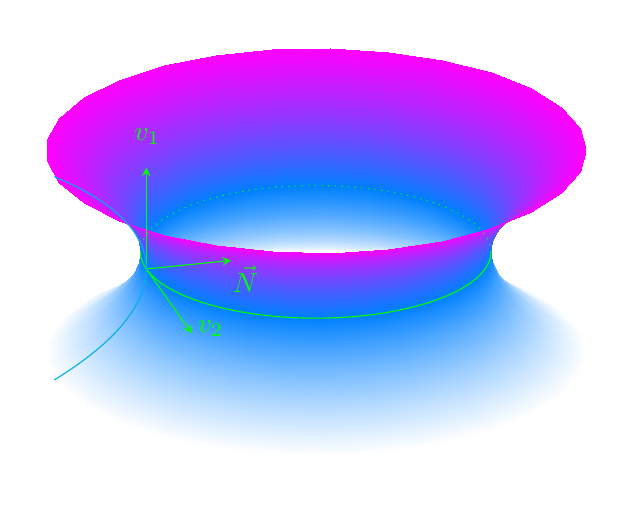
\begin{tikzpicture}
            \begin{axis}[xticklabels={,,},%不显示x坐标轴数字
                    yticklabels={,,},
                    zticklabels={,,},
                    axis line style={draw=none},%不显示坐标轴
                    tick style={draw=none},
                    colormap/cool,
                    view={0}{40}
                    ]
                \addplot3 [
                surf,
                shader=interp,
                z buffer=sort,
                domain=0:360, domain y=-1:1,
                samples=30, samples y=30,
                variable=\v, variable y=\u,
                %point meta=u
                ] ({cosh(u)*cos(v)},
                {cosh(u)*sin(v)},
                {u});
                \addplot3 [
                    green,
                    quiver={u=\thisrow{u},v=\thisrow{v},w=\thisrow{w}},
                    -stealth,
                ] table{
                    x y z u v w 
                    -0.96592582628 -0.2588190451 0 0 0 1 
                    -0.96592582628 -0.2588190451 0 0.2588190451 -0.96592582628 0 
                    -0.96592582628 -0.2588190451 0 0.48296291314 0.12940952255 0 
                };
                \addplot3 [
                    green,
                    domain=-180:0,
                    samples=40,
                    samples y=1%防止曲线闭合
                ]({cos(x)},{sin(x)},0);
                \addplot3 [
                    green,
                    dotted,
                    domain=0:180,
                    samples=40,
                    samples y=1%防止曲线闭合
                ]({cos(x)},{sin(x)},0);
                \addplot3 [
                    cyan,
                    domain=-1:1,
                    variable=\t,
                    samples=40,
                    samples y=1
                ]({cosh(t)*-0.96592582628},{cosh(t)*-0.2588190451},{t});
                \node[text=green] at (-0.96,-0.25,1.3) {\(v_1\)};
                \node[text=green] at (-0.60,-1.15,0) {\(v_2\)};
                \node[text=green] at (-0.4,-0.1,-0.2) {\(\vec{N}\)};
            \end{axis}
        \end{tikzpicture}
        \end{center}
    As you may notice, in \cref{normal curvature-sphere}, all 
    normal curvatures are the same at all points and along any 
    direction. In \cref{normal curvature-cylinder} and 
    \cref{normal curvature-catenoid}, at any point there are extremal
    directions at which the normal curvature achieves 
    the maximum and the minimum. Let's discuss more on these two special 
    normal curvatures.
\subsection{Principle curvature and principle direction}
Since \(\dd N_p\colon T_p S\to T_p S\) is linear and 
symmetric (self-adjoint), for any orthonormal basis {\(e_1,e_2\)},
\[
        \dd N_p\begin{pmatrix}
            e_1\\
            e_2
        \end{pmatrix}
        =\underbrace{\begin{pmatrix}
            a_{11}&a_{12}\\
            a_{21}&a_{22}
        \end{pmatrix}}_{symmetric}
        \begin{pmatrix}
            e_1\\
            e_2
        \end{pmatrix}
\]
\(\Rightarrow \exists\) an orthonormal basis {\(\tilde{e_1}
,\tilde{e_2}\)} of \(T_p S\) such that 
\[
        \dd{N}_p \begin{pmatrix}
            \tilde{e_1}\\
            \tilde{e_2}
        \end{pmatrix}
        =\begin{pmatrix}
            -k_1& 0\\
            0&-k_2
        \end{pmatrix}\begin{pmatrix}
            \tilde{e_1}\\
            \tilde{e_2}
        \end{pmatrix}
        \quad (k_1\ge k_2)
\]
\begin{definition}[Principle curvature and principle direction]
    \(k_1\) and \(k_2\) above are called the principle curvature
    and \(\tilde{e_1},\tilde{e_2}\) are called the principle
    directions at \(p\).
\end{definition}
\begin{remark}
    \(k_1\) and \(k_2\) are the maximum and minimum values of 
    the \engordnumber{2} fundamental form \(\II\) restricted on 
    the unit vectors of \(T_p S\).
\end{remark}
\begin{proof}
    \[
    \II\left(\tilde{e_1},\tilde{e_1}\right)=-\left\langle
        \dd N_p\left(\tilde{e_1}\right),\tilde{e_1}\right\rangle
        =\left\langle k_1 \tilde{e_1},\tilde{e_1}\right\rangle
        =k_1.
    \]
    Similarly, \(\II\left(\tilde{e_2},\tilde{e_2}\right)=k_2\).

    For any unit vector \(v\in T_p S\), \(v=
    v_1\tilde{e_1}+v_2\tilde{e_2}\), with \(|v|=1\).
    \begin{align*}
        \II(v,v)&=-\left\langle \dd N_p(v),v\right\rangle\\
        &=-\left\langle v_1 \dd N_p\left(\tilde{e_1}\right)
        +v_2\dd N_p\left(\tilde{e_2}\right),v_1\tilde{e_1}+v_2
        \tilde{e_2}\right\rangle\\
        &=k_1 v_1^2 +k_2 v_2^2=
        \begin{cases}
            k_1+(k_1-k_2)v_2^2\le k_1,\\
            (k_1-k_2)v_1^2+k_2\ge k_2.
        \end{cases}
    \end{align*}
    Hence, \(k_1\) and \(k_2\) are maximum and minimum values of normal
    curvature. Moreover, \(\forall\) unit vector \(v\in T_p S\) and 
    {\(e_1,e_2\)} the principle direction, we can write
    \[
        v=\cos \theta e_1+\sin\theta e_2,
    \]
    \[
        k_{\vb{n}}(v)=k_1 \cos^2\theta +k_2 \sin^2\theta.    
    \]
    The last is called ``Euler formula''.
\end{proof}

%==============================%

% \printbibliography{}
\end{document}
